\chapter{Continuous contrast variation applied to relevant bio-materials}
\label{chap:bio_applications}

In the continuously growing world of nanotechnology, nanoscience provides understanding for biological structures at the nanometer length scale, such as lipoprotein biology, while the application of nanoparticles in medicine opens exciting new possibilities in this field \cite{nie_nanotechnology_2007, sahoo_nanotech_2003, wickline_nanotechnology_2003, zhou_nano-enabled_2014, rosen_rise_2005}. For example, polymeric colloids and other biodegradable nanocarriers are finding many medical applications\citep{vicent_polymer_2006} and are starting to undergo clinical trials\citep{patel_polymeric_2012,beija_colloidal_2012,cabral_progress_2014}. 

In this sense, liposomes have an increasing importance in the emerging field of nanomedicine, due to their capacity to encapsulate hydrophillic compounds within the closed phospholipid bilayer membrane. The first approved nanodrug, Caelyx$\textregistered$, consists of a PEGylated liposomal formulation of doxorubicin. In fact, liposomal nanocarriers are nowadays a widespread instrument for drug delivery.

Despite SAXS being a usual method of choice for the accurate characterization of nanomaterials, the interpretation of the scattering curves, i.e. the uniqueness of the solution of the model fitting, is frequently intricate for complex samples. Liposomal drugs or loaded polymeric nanoparticles belong to this class, as both the carrier and the incorporated biotarget contribute to the scattering intensity. 

Therefore, the characterization of NPs with a broad size distribution, a heterogeneous composition or with a complicated inner structure require either \emph{a priori} knowledge about the morphology of the sample or the measurement of complementary scattering curves obtained under different experimental conditions, like in solvent contrast variation in SAXS 

In this chapter, the utilization of continuous contrast variation in SAXS is examined for the nanodrug Caelyx$\textregistered$ and for typical nanocarriers like lipid vesicles or polymeric colloids. In the latter case, the particle is coated with an antibody to resemble the biological conditions found upon injection in the bloodstream. Other components of the blood plasma like lipoproteins are also investigated with this technique.


\section{Materials and methods}

The continouous contrast variation method in SAXS has been employed in a variety of samples related with nanomedicine. In this section, the different samples characterized with this technique are described and the more relevant aspects of the experiments are detailed. The results obtained on the Caelyx$\textregistered$ nanodrug are described principally in section \ref{sec:caelyx_size} and \ref{sec:OsmoticCaelyx}, while the empty liposomes are investigated under osmotic pressure in section \ref{sec:liposome_osmotic}. The size measurements on the lipoproteins are presented in section \ref{sec:lipoprotein_continuous} and the use of the protein-coated nanoparticles is detailed in section \ref{sec:CoatedKiskerExperimental}.

\subsection{Caelyx$\textregistered$: PEGylated liposomal doxorubicin}
\label{sec:materials_caelyx}
The PEGylated liposomal formulation of doxorubicin, Caelyx$\textregistered$ (SP Europe, Brussels, Belgium), was purchased from Hungaropharma Ltd. Caelyx $\textregistered$ (or Doxil $\textregistered$ in US) consist of liposomes formed by fully hydrogenated soy phosphatydilcholine (HSPC), cholesterol, and DSPE-PEG2000 (N-(carbonyl-methoxypolyethylene glycol 2000)-1,2-distearoyl-sn-glycero-3-phosphoethanolamine). The latter results a steric barrier at the liposomal surface due to the PEG 2000 residues. Doxorubicin is encapsulated in Caelyx $\textregistered$ via an active loading procedure, which results a crystal-like doxorubicin precipitate inside the liposomes, as observed in the micrograph \ref{fig:CaelyxCryoTEM}. An schematic depiction of the sample morphology is shown in figure \ref{fig:CaelyxScheme}. 

\begin{figure}
	\centering
		\subfloat[Cryo-TEM]{\resizebox{0.4\linewidth}{!}{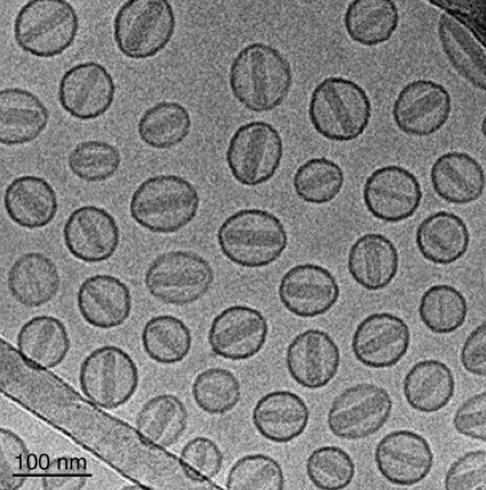
\includegraphics{Figures/CaelyxCryoTEM.png}}\label{fig:CaelyxCryoTEM}}
		\subfloat[Scheme]{\def\svgwidth{0.7\linewidth}{\input{Figures/CaelyxScheme.pdf_tex}}\label{fig:CaelyxScheme}}
		\caption{Cryo-TEM image of Caelyx$\textregistered$ \cite{barenholz_doxil_2012} and schematic representation of the PEGylated liposomal doxorubicin morphology \cite{garcia-diez_size_2016}.}
\end{figure}

The suspending medium contrast variation study was performed with the iso-osmolar contrast agent Optiprep $\textregistered$ (an aqueous solution of iodixanol), which has an osmolality of 290 to 310 mOsm kg$^{-1}$. The suspending medium density gradient was achieved by bringing together two mixtures of different densities: For the bottom of the capillary, a high density mixture of Caelyx $\textregistered$ was prepared with an Optiprep $\textregistered$ mass fraction of 35 $\%$ and a corresponding solvent electron density of 365.2 nm$^{-3}$, whilst on the top side of the capillary a low density preparation of Caelyx $\textregistered$  using phosphate buffered saline solution (pH 7.4) with the same volume fraction of Caelyx $\textregistered$ was introduced, with a solvent electron density of 341.9 nm$^{-3}$. By employing Optiprep $\textregistered$ as a contrast agent, the suspending medium osmolality is constant along the capillary. 

In order to study the effects of the suspending medium osmolality in the liposomal drug carrier, another capillary with a density gradient was created by introducing a dense aqueous sucrose solution with 37.8 $\%$ sucrose mass fraction (Sigma-Aldrich, Missouri, USA) at the bottom of the capillary (which corresponds to an electron density of 381.1 nm$^{-3}$ and a solvent osmolality of 1775.6 mOsm kg$^{-1}$), whereas a lighter solution was produced without sucrose by adding pure water to get the same Caelyx $\textregistered$ concentration. Considering the sucrose mass fraction of the Caelyx® buffer to be 10$\%$, this latter preparation has an electron density of 339.4 nm$^{-3}$ and an osmolality of 151.1 mOsm kg$^{-1}$. 

A wide-angle configuration was employed to observe the diffraction peak of the fiber-like doxorubicin precipitate encapsulated in the liposomes. At this configuration, the sample-to-detector distance was reduced to $L = (569 \pm  1)$ mm and as a result the available $q$-range was extended until 5.55 nm$^{-1}$. For the wide-angle X-ray scattering measurements, a density gradient capillary was prepared using a denser aqueous solution with a sucrose mass fraction of 34$\%$ and a lighter one with 6$\%$.

%\begin{figure}
%	\centering
%		% GNUPLOT: LaTeX picture with Postscript
\begingroup
  \makeatletter
  \providecommand\color[2][]{%
    \GenericError{(gnuplot) \space\space\space\@spaces}{%
      Package color not loaded in conjunction with
      terminal option `colourtext'%
    }{See the gnuplot documentation for explanation.%
    }{Either use 'blacktext' in gnuplot or load the package
      color.sty in LaTeX.}%
    \renewcommand\color[2][]{}%
  }%
  \providecommand\includegraphics[2][]{%
    \GenericError{(gnuplot) \space\space\space\@spaces}{%
      Package graphicx or graphics not loaded%
    }{See the gnuplot documentation for explanation.%
    }{The gnuplot epslatex terminal needs graphicx.sty or graphics.sty.}%
    \renewcommand\includegraphics[2][]{}%
  }%
  \providecommand\rotatebox[2]{#2}%
  \@ifundefined{ifGPcolor}{%
    \newif\ifGPcolor
    \GPcolortrue
  }{}%
  \@ifundefined{ifGPblacktext}{%
    \newif\ifGPblacktext
    \GPblacktextfalse
  }{}%
  % define a \g@addto@macro without @ in the name:
  \let\gplgaddtomacro\g@addto@macro
  % define empty templates for all commands taking text:
  \gdef\gplbacktext{}%
  \gdef\gplfronttext{}%
  \makeatother
  \ifGPblacktext
    % no textcolor at all
    \def\colorrgb#1{}%
    \def\colorgray#1{}%
  \else
    % gray or color?
    \ifGPcolor
      \def\colorrgb#1{\color[rgb]{#1}}%
      \def\colorgray#1{\color[gray]{#1}}%
      \expandafter\def\csname LTw\endcsname{\color{white}}%
      \expandafter\def\csname LTb\endcsname{\color{black}}%
      \expandafter\def\csname LTa\endcsname{\color{black}}%
      \expandafter\def\csname LT0\endcsname{\color[rgb]{1,0,0}}%
      \expandafter\def\csname LT1\endcsname{\color[rgb]{0,1,0}}%
      \expandafter\def\csname LT2\endcsname{\color[rgb]{0,0,1}}%
      \expandafter\def\csname LT3\endcsname{\color[rgb]{1,0,1}}%
      \expandafter\def\csname LT4\endcsname{\color[rgb]{0,1,1}}%
      \expandafter\def\csname LT5\endcsname{\color[rgb]{1,1,0}}%
      \expandafter\def\csname LT6\endcsname{\color[rgb]{0,0,0}}%
      \expandafter\def\csname LT7\endcsname{\color[rgb]{1,0.3,0}}%
      \expandafter\def\csname LT8\endcsname{\color[rgb]{0.5,0.5,0.5}}%
    \else
      % gray
      \def\colorrgb#1{\color{black}}%
      \def\colorgray#1{\color[gray]{#1}}%
      \expandafter\def\csname LTw\endcsname{\color{white}}%
      \expandafter\def\csname LTb\endcsname{\color{black}}%
      \expandafter\def\csname LTa\endcsname{\color{black}}%
      \expandafter\def\csname LT0\endcsname{\color{black}}%
      \expandafter\def\csname LT1\endcsname{\color{black}}%
      \expandafter\def\csname LT2\endcsname{\color{black}}%
      \expandafter\def\csname LT3\endcsname{\color{black}}%
      \expandafter\def\csname LT4\endcsname{\color{black}}%
      \expandafter\def\csname LT5\endcsname{\color{black}}%
      \expandafter\def\csname LT6\endcsname{\color{black}}%
      \expandafter\def\csname LT7\endcsname{\color{black}}%
      \expandafter\def\csname LT8\endcsname{\color{black}}%
    \fi
  \fi
  \setlength{\unitlength}{0.0500bp}%
  \begin{picture}(5668.00,4534.00)%
    \gplgaddtomacro\gplbacktext{%
      \csname LTb\endcsname%
      \put(946,1162){\makebox(0,0)[r]{\strut{} 1}}%
      \put(946,2313){\makebox(0,0)[r]{\strut{} 10}}%
      \put(946,3464){\makebox(0,0)[r]{\strut{} 100}}%
      \put(2391,484){\makebox(0,0){\strut{} 0.1}}%
      \put(5271,484){\makebox(0,0){\strut{} 1}}%
      \put(176,2486){\rotatebox{-270}{\makebox(0,0){\strut{}Scattering Intensity / a.u.}}}%
      \put(3174,154){\makebox(0,0){\strut{}$q$ / nm$^{-1}$}}%
    }%
    \gplgaddtomacro\gplfronttext{%
      \csname LTb\endcsname%
      \put(4284,4096){\makebox(0,0)[r]{\strut{}Caelyx in buffer}}%
      \csname LTb\endcsname%
      \put(4284,3876){\makebox(0,0)[r]{\strut{}Caelyx in 9.1$\%$ iodixanol}}%
      \csname LTb\endcsname%
      \put(4284,3656){\makebox(0,0)[r]{\strut{}SSL in buffer}}%
      \csname LTb\endcsname%
      \put(4284,3436){\makebox(0,0)[r]{\strut{}Vesicle fit}}%
    }%
    \gplbacktext
    \put(0,0){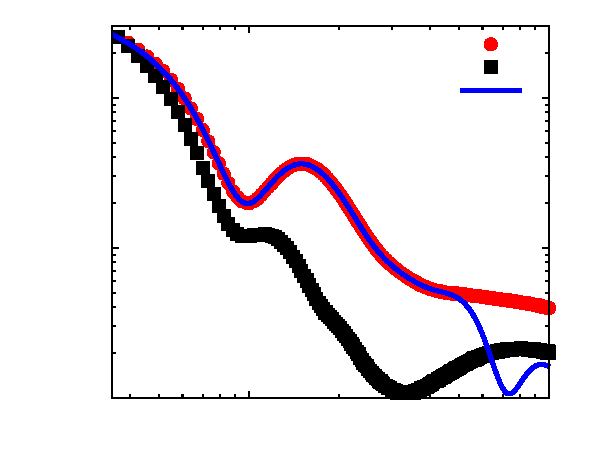
\includegraphics{CaelyxIodixanolSingleContrast}}%
    \gplfronttext
  \end{picture}%
\endgroup

%		\caption{Caelyx$\textregistered$ in buffer and in 9.1 $\%$ iodixanol: SAXS scattering curve at single contrast compared to that of a PEGylated liposome of similar size.}
%		\label{fig:CaelyxIodixanolSingleContrast}
%\end{figure}

\subsection{Lipid vesicles: PEGylated and plain liposomes}
\label{sec:materials_liposome}

The PEGylated liposomes were prepared with the same lipid composition that the commercially available Caelyx $\textregistered$ for comparison purposes: the weight ratios of HSPC:DSPE-PEG 2000:cholesterol were 3:1:1 (corresponding to molar ratios of 0.565:0.053:0.382). The samples were extruded through polycarbonate filters (Nucleopore, Whatman Inc., Little Chalfont, UK) of 5 different pore sizes, from 50 to 400 nm. A more detailed description of the preparation is found elsewhere \cite{varga_osmotic_2014}. The components of the plain liposomes are \textcolor{red}{HSPC:cholesterol with a weight ratio of X:Y (corresponding to a molar ratio of X:Y). The preparation is identical to the PEGylated liposomes.} All the liposome samples are suspended in a 10 mM Tris pH 7.4 buffer solution.

The DLS size measurements were performed on a W130i apparatus (Avid Nano Ltd, High Wycombe, UK) in the Institute of Materials and Environmental Chemistry (Hungarian Academy of Sciences, Budapest, Hungary) similarly to the protocol described in \cite{varga_osmotic_2014}. The samples sizes employed in the discussion of section \ref{sec:liposome_osmotic} are the \textcolor{red}{intensity-weighted} results from these measurements. It is apparent from these measurements that the size of the pore and the polydispersity degree of the liposome sample are directly related.

The concentration of sucrose employed to constitute the high-density phase of the different density gradients is detailed in the discussion of section \ref{sec:liposome_osmotic}. The top-part of the capillary was filled with a diluted preparation of the sample in buffer to match the liposome concentration in the bottom phase.

\subsection{Human lipoproteins}

Native lipoproteins from human plasma were purchased from Merck Milipore (Darmstadt, Deutschland) and suspended in 150 mM NaCl, 0.01 $\%$ EDTA buffer with pH 7.4. The High Density Lipoprotein (HDL) had a protein concentration of 14.3 g/L, while the Low Density Lipoprotein (LDL) had a protein concentration of 5.96 g/L, considering that the weight ratio between lipids and proteins is approximately 4:1 in the LDL sample. 

\begin{figure}
	\centering
		% GNUPLOT: LaTeX picture with Postscript
\begingroup
  \makeatletter
  \providecommand\color[2][]{%
    \GenericError{(gnuplot) \space\space\space\@spaces}{%
      Package color not loaded in conjunction with
      terminal option `colourtext'%
    }{See the gnuplot documentation for explanation.%
    }{Either use 'blacktext' in gnuplot or load the package
      color.sty in LaTeX.}%
    \renewcommand\color[2][]{}%
  }%
  \providecommand\includegraphics[2][]{%
    \GenericError{(gnuplot) \space\space\space\@spaces}{%
      Package graphicx or graphics not loaded%
    }{See the gnuplot documentation for explanation.%
    }{The gnuplot epslatex terminal needs graphicx.sty or graphics.sty.}%
    \renewcommand\includegraphics[2][]{}%
  }%
  \providecommand\rotatebox[2]{#2}%
  \@ifundefined{ifGPcolor}{%
    \newif\ifGPcolor
    \GPcolortrue
  }{}%
  \@ifundefined{ifGPblacktext}{%
    \newif\ifGPblacktext
    \GPblacktextfalse
  }{}%
  % define a \g@addto@macro without @ in the name:
  \let\gplgaddtomacro\g@addto@macro
  % define empty templates for all commands taking text:
  \gdef\gplbacktext{}%
  \gdef\gplfronttext{}%
  \makeatother
  \ifGPblacktext
    % no textcolor at all
    \def\colorrgb#1{}%
    \def\colorgray#1{}%
  \else
    % gray or color?
    \ifGPcolor
      \def\colorrgb#1{\color[rgb]{#1}}%
      \def\colorgray#1{\color[gray]{#1}}%
      \expandafter\def\csname LTw\endcsname{\color{white}}%
      \expandafter\def\csname LTb\endcsname{\color{black}}%
      \expandafter\def\csname LTa\endcsname{\color{black}}%
      \expandafter\def\csname LT0\endcsname{\color[rgb]{1,0,0}}%
      \expandafter\def\csname LT1\endcsname{\color[rgb]{0,1,0}}%
      \expandafter\def\csname LT2\endcsname{\color[rgb]{0,0,1}}%
      \expandafter\def\csname LT3\endcsname{\color[rgb]{1,0,1}}%
      \expandafter\def\csname LT4\endcsname{\color[rgb]{0,1,1}}%
      \expandafter\def\csname LT5\endcsname{\color[rgb]{1,1,0}}%
      \expandafter\def\csname LT6\endcsname{\color[rgb]{0,0,0}}%
      \expandafter\def\csname LT7\endcsname{\color[rgb]{1,0.3,0}}%
      \expandafter\def\csname LT8\endcsname{\color[rgb]{0.5,0.5,0.5}}%
    \else
      % gray
      \def\colorrgb#1{\color{black}}%
      \def\colorgray#1{\color[gray]{#1}}%
      \expandafter\def\csname LTw\endcsname{\color{white}}%
      \expandafter\def\csname LTb\endcsname{\color{black}}%
      \expandafter\def\csname LTa\endcsname{\color{black}}%
      \expandafter\def\csname LT0\endcsname{\color{black}}%
      \expandafter\def\csname LT1\endcsname{\color{black}}%
      \expandafter\def\csname LT2\endcsname{\color{black}}%
      \expandafter\def\csname LT3\endcsname{\color{black}}%
      \expandafter\def\csname LT4\endcsname{\color{black}}%
      \expandafter\def\csname LT5\endcsname{\color{black}}%
      \expandafter\def\csname LT6\endcsname{\color{black}}%
      \expandafter\def\csname LT7\endcsname{\color{black}}%
      \expandafter\def\csname LT8\endcsname{\color{black}}%
    \fi
  \fi
    \setlength{\unitlength}{0.0500bp}%
    \ifx\gptboxheight\undefined%
      \newlength{\gptboxheight}%
      \newlength{\gptboxwidth}%
      \newsavebox{\gptboxtext}%
    \fi%
    \setlength{\fboxrule}{0.5pt}%
    \setlength{\fboxsep}{1pt}%
\begin{picture}(5668.00,4534.00)%
    \gplgaddtomacro\gplbacktext{%
      \csname LTb\endcsname%
      \put(594,1164){\makebox(0,0)[r]{\strut{}$1$}}%
      \csname LTb\endcsname%
      \put(594,2489){\makebox(0,0)[r]{\strut{}$10$}}%
      \csname LTb\endcsname%
      \put(594,3815){\makebox(0,0)[r]{\strut{}$100$}}%
      \csname LTb\endcsname%
      \put(1074,484){\makebox(0,0){\strut{}$0.3$}}%
      \csname LTb\endcsname%
      \put(1743,484){\makebox(0,0){\strut{}$0.5$}}%
      \csname LTb\endcsname%
      \put(2650,484){\makebox(0,0){\strut{}$1$}}%
      \csname LTb\endcsname%
      \put(4089,484){\makebox(0,0){\strut{}$3$}}%
      \csname LTb\endcsname%
      \put(4758,484){\makebox(0,0){\strut{}$5$}}%
    }%
    \gplgaddtomacro\gplfronttext{%
      \csname LTb\endcsname%
      \put(220,2486){\rotatebox{-270}{\makebox(0,0){\strut{}Scattering Intensity / a.u.}}}%
      \put(2998,154){\makebox(0,0){\strut{}$q$ / nm$^{-1}$}}%
      \csname LTb\endcsname%
      \put(4284,4096){\makebox(0,0)[r]{\strut{}Experimental}}%
      \csname LTb\endcsname%
      \put(4284,3876){\makebox(0,0)[r]{\strut{}Model Fit}}%
    }%
    \gplbacktext
    \put(0,0){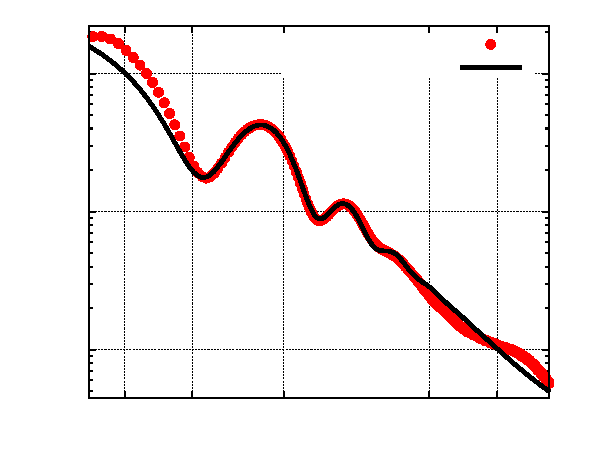
\includegraphics{HDLCoreShellFit}}%
    \gplfronttext
  \end{picture}%
\endgroup

		\caption{Scattering curve of HDL: A core-shell model is fitted to the experimental data (red symbols) resulting in an outer diameter of 9.7 nm and a core radius of 4.2 nm.}
		\label{fig:HDLCoreShellFit}
\end{figure}

In figure \ref{fig:HDLCoreShellFit}, a single-contrast SAXS curve of HDL in buffer is displayed, where the best fit of a core-shell model is also shown. It is evident that the fit does not match the data correctly and, thus, the mophology of the lipoprotein cannot be described with a simple core-shell model. The complementary measurements were performed by continuous contrast variation in SAXS using sucrose as contrast agent. The maximum sucrose mass fraction employed in the preparation of the density gradients was 40 $\%$, as detailed in section \ref{sec:lipoprotein_continuous}.

\subsection{PS-COOH particles coated with IgG}

The polystyrene nanoparticles with carboxylated surfaces (PS-COOH) described in section \textcolor{red}{WHICH ONE????} are coated with the protein Immunoglobulin G (IgG). A set of four IgG-coated polystyrene nanoparticle samples was prepared by incubating 0.05 $\%$ (w/w) particles with varying concentrations of IgG from 0.5 to 4 g/L in 100 mM Tris buffer at pH 8 under continuous shaking for 2 h. Any unbound IgG was then removed from the particle samples by three cycles of centrifugation and redispersion in clean buffer. 

In the continuous contrast variation experiment with sucrose as contrast agent, a protein concentration of 4 g/L IgG was physisorbed at the surface of the bare PS-COOH particles. The details of the density gradient capillary are discussed in section \ref{sec:coated_kisker_continuous}.


\section{Traceable size determination of a liposomal drug}
\label{sec:caelyx_size}

The first approved nano-drug was Doxil$\textregistered$ (Caelyx$\textregistered$ in Europe), a PEGylated liposomal formulation of doxorubicin, which was followed by a few other products\cite{yeh_clinical_2011,barenholz_doxil_2012}. Nowadays there are approximately 250 nanomedicine products that are either approved by the relevant health agencies or are under clinical trials \cite{etheridge_big_2013}. On the other hand, there is a translational gap between the experimental work devoted to the development of new nano-drug candidates and the clinical realization of their use, which is also reflected in the high number of studies dealing with nanomedicine and the number of approved products on the market \cite{khorasani_closing_2014, venditto_cancer_2013}. As highlighted in a recent review by \cite{khorasani_closing_2014}, one of the main reasons for this translational gap is that the current characterization techniques possess limitations and there is a need for standardization on this field.

Among many relevant physicochemical properties of nano-drugs, one of the most important to be accurately determined is the size of the nanocarriers, which directly relates to the in vivo biodistribution of the drug. The ultimate goal in this regard is to reach a "traceable size determination" of the nanomaterial, which means that the measurand can be related to the SI unit "meter" through an unbroken chain of comparisons with known uncertainties. 

The most widely used technique for size determination in the field of nanomedicine is dynamic light scattering (DLS), which measures the hydrodynamic diameter of the nanoparticles (NPs) \cite{murphy_static_1997, hallett_vesicle_1991, egelhaaf_determination_1996, takahashi_precise_2008, jans_dynamic_2009, hoo_comparison_2008}. DLS is well-established and has indisputable advantages in the size characterization of the NPs, e.g. easy-to-use instrumentations, fast and low-cost operation, but it is not capable of a traceable size determination as there is no general relationship between the hydrodynamic diameter and the physical size of the NPs \cite{meli_traceable_2012}. 

Transmission electron microscopy (TEM) is also frequently used for sizing of NPs and proved to be an appropriate technique for solid nanoparticles, whilst its employment in soft matter NPs (e.g. liposomes, micelles and polymeric nanoparticles) is questionable due to the possible distortion of the particles during the drying process.  Although cryo-TEM could overcome this limitation \cite{li_doxorubicin_1998}, the statistical accuracy of this non-ensemble method is usually not sufficient.

SAXS is capable of traceable size determination for sufficiently monodisperse nanoparticles \cite{meli_traceable_2012} and therefore the continuous contrast variation technique with SAXS is a suitable method to assess the size of a complex liposomal drug, such as the PEGylated liposomal formulation of doxorubicin. The need of an iso-osmolal suspending medium to mimic the phyisiological conditions of plasma requires the use of Optiprep $\textregistered$ as contrast agent, as explained in section \ref{sec:materials_caelyx}.
 
SAXS curves of the liposomal doxorubicin sample measured at different suspending medium electron densities are shown in figure \ref{fig:CaelyxIodixanolContinuousSAXS}. In the scattering curves, it is possible to observe the variation of the curve features through the increase of the suspending medium density, which indicates the complexity of the internal structure of the nanocarrier. Besides, the appearance of an intersection point around $q = 0.12$ nm$^{-1}$ is a further indicator of the structural complexity of the drug-carrier.

\begin{figure}
	\centering
		\subfloat[Contrast variation with density gradient]{\resizebox{0.44\linewidth}{!}{% GNUPLOT: LaTeX picture with Postscript
\begingroup
  \makeatletter
  \providecommand\color[2][]{%
    \GenericError{(gnuplot) \space\space\space\@spaces}{%
      Package color not loaded in conjunction with
      terminal option `colourtext'%
    }{See the gnuplot documentation for explanation.%
    }{Either use 'blacktext' in gnuplot or load the package
      color.sty in LaTeX.}%
    \renewcommand\color[2][]{}%
  }%
  \providecommand\includegraphics[2][]{%
    \GenericError{(gnuplot) \space\space\space\@spaces}{%
      Package graphicx or graphics not loaded%
    }{See the gnuplot documentation for explanation.%
    }{The gnuplot epslatex terminal needs graphicx.sty or graphics.sty.}%
    \renewcommand\includegraphics[2][]{}%
  }%
  \providecommand\rotatebox[2]{#2}%
  \@ifundefined{ifGPcolor}{%
    \newif\ifGPcolor
    \GPcolortrue
  }{}%
  \@ifundefined{ifGPblacktext}{%
    \newif\ifGPblacktext
    \GPblacktextfalse
  }{}%
  % define a \g@addto@macro without @ in the name:
  \let\gplgaddtomacro\g@addto@macro
  % define empty templates for all commands taking text:
  \gdef\gplbacktext{}%
  \gdef\gplfronttext{}%
  \makeatother
  \ifGPblacktext
    % no textcolor at all
    \def\colorrgb#1{}%
    \def\colorgray#1{}%
  \else
    % gray or color?
    \ifGPcolor
      \def\colorrgb#1{\color[rgb]{#1}}%
      \def\colorgray#1{\color[gray]{#1}}%
      \expandafter\def\csname LTw\endcsname{\color{white}}%
      \expandafter\def\csname LTb\endcsname{\color{black}}%
      \expandafter\def\csname LTa\endcsname{\color{black}}%
      \expandafter\def\csname LT0\endcsname{\color[rgb]{1,0,0}}%
      \expandafter\def\csname LT1\endcsname{\color[rgb]{0,1,0}}%
      \expandafter\def\csname LT2\endcsname{\color[rgb]{0,0,1}}%
      \expandafter\def\csname LT3\endcsname{\color[rgb]{1,0,1}}%
      \expandafter\def\csname LT4\endcsname{\color[rgb]{0,1,1}}%
      \expandafter\def\csname LT5\endcsname{\color[rgb]{1,1,0}}%
      \expandafter\def\csname LT6\endcsname{\color[rgb]{0,0,0}}%
      \expandafter\def\csname LT7\endcsname{\color[rgb]{1,0.3,0}}%
      \expandafter\def\csname LT8\endcsname{\color[rgb]{0.5,0.5,0.5}}%
    \else
      % gray
      \def\colorrgb#1{\color{black}}%
      \def\colorgray#1{\color[gray]{#1}}%
      \expandafter\def\csname LTw\endcsname{\color{white}}%
      \expandafter\def\csname LTb\endcsname{\color{black}}%
      \expandafter\def\csname LTa\endcsname{\color{black}}%
      \expandafter\def\csname LT0\endcsname{\color{black}}%
      \expandafter\def\csname LT1\endcsname{\color{black}}%
      \expandafter\def\csname LT2\endcsname{\color{black}}%
      \expandafter\def\csname LT3\endcsname{\color{black}}%
      \expandafter\def\csname LT4\endcsname{\color{black}}%
      \expandafter\def\csname LT5\endcsname{\color{black}}%
      \expandafter\def\csname LT6\endcsname{\color{black}}%
      \expandafter\def\csname LT7\endcsname{\color{black}}%
      \expandafter\def\csname LT8\endcsname{\color{black}}%
    \fi
  \fi
    \setlength{\unitlength}{0.0500bp}%
    \ifx\gptboxheight\undefined%
      \newlength{\gptboxheight}%
      \newlength{\gptboxwidth}%
      \newsavebox{\gptboxtext}%
    \fi%
    \setlength{\fboxrule}{0.5pt}%
    \setlength{\fboxsep}{1pt}%
\begin{picture}(5668.00,4534.00)%
    \gplgaddtomacro\gplbacktext{%
      \csname LTb\endcsname%
      \put(814,1234){\makebox(0,0)[r]{\strut{}$0.01$}}%
      \csname LTb\endcsname%
      \put(814,1993){\makebox(0,0)[r]{\strut{}$0.1$}}%
      \csname LTb\endcsname%
      \put(814,2752){\makebox(0,0)[r]{\strut{}$1$}}%
      \csname LTb\endcsname%
      \put(814,3510){\makebox(0,0)[r]{\strut{}$10$}}%
      \csname LTb\endcsname%
      \put(814,4269){\makebox(0,0)[r]{\strut{}$100$}}%
      \csname LTb\endcsname%
      \put(1453,484){\makebox(0,0){\strut{}$0.05$}}%
      \csname LTb\endcsname%
      \put(2142,484){\makebox(0,0){\strut{}$0.1$}}%
      \csname LTb\endcsname%
      \put(2830,484){\makebox(0,0){\strut{}$0.2$}}%
      \csname LTb\endcsname%
      \put(3741,484){\makebox(0,0){\strut{}$0.5$}}%
      \csname LTb\endcsname%
      \put(4429,484){\makebox(0,0){\strut{}$1$}}%
    }%
    \gplgaddtomacro\gplfronttext{%
      \csname LTb\endcsname%
      \put(176,2266){\rotatebox{-270}{\makebox(0,0){\strut{}Scattering Intensity / cm$^{-1}$}}}%
      \put(2687,154){\makebox(0,0){\strut{}$q$ / nm$^{-1}$}}%
      \csname LTb\endcsname%
      \put(4691,1149){\makebox(0,0)[l]{\strut{}\smaller 345}}%
      \put(4691,1892){\makebox(0,0)[l]{\strut{}\smaller 350}}%
      \put(4691,2635){\makebox(0,0)[l]{\strut{}\smaller 355}}%
      \put(4691,3377){\makebox(0,0)[l]{\strut{}\smaller 360}}%
      \put(4691,4120){\makebox(0,0)[l]{\strut{}\smaller 365}}%
      \put(5351,2486){\rotatebox{-90}{\makebox(0,0){\strut{}\smaller Solvent Electron Density / nm$^{-3}$}}}%
    }%
    \gplbacktext
    \put(0,0){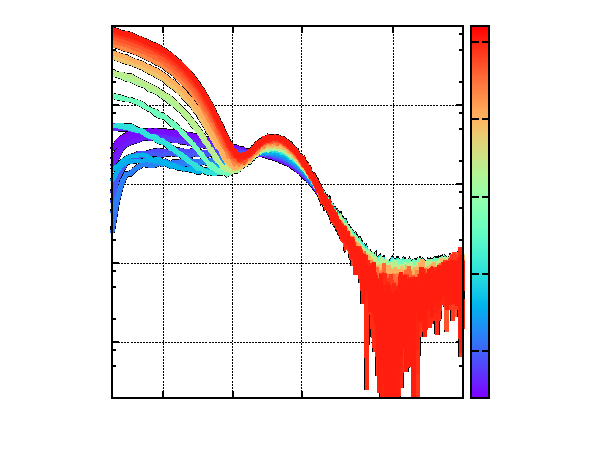
\includegraphics{CaelyxIodixanolContinuousSAXS}}%
    \gplfronttext
  \end{picture}%
\endgroup
}\label{fig:CaelyxIodixanolContinuousSAXS}}
		\subfloat[Isoscattering point positions]{\resizebox{0.44\linewidth}{!}{% GNUPLOT: LaTeX picture with Postscript
\begingroup
  \makeatletter
  \providecommand\color[2][]{%
    \GenericError{(gnuplot) \space\space\space\@spaces}{%
      Package color not loaded in conjunction with
      terminal option `colourtext'%
    }{See the gnuplot documentation for explanation.%
    }{Either use 'blacktext' in gnuplot or load the package
      color.sty in LaTeX.}%
    \renewcommand\color[2][]{}%
  }%
  \providecommand\includegraphics[2][]{%
    \GenericError{(gnuplot) \space\space\space\@spaces}{%
      Package graphicx or graphics not loaded%
    }{See the gnuplot documentation for explanation.%
    }{The gnuplot epslatex terminal needs graphicx.sty or graphics.sty.}%
    \renewcommand\includegraphics[2][]{}%
  }%
  \providecommand\rotatebox[2]{#2}%
  \@ifundefined{ifGPcolor}{%
    \newif\ifGPcolor
    \GPcolortrue
  }{}%
  \@ifundefined{ifGPblacktext}{%
    \newif\ifGPblacktext
    \GPblacktextfalse
  }{}%
  % define a \g@addto@macro without @ in the name:
  \let\gplgaddtomacro\g@addto@macro
  % define empty templates for all commands taking text:
  \gdef\gplbacktext{}%
  \gdef\gplfronttext{}%
  \makeatother
  \ifGPblacktext
    % no textcolor at all
    \def\colorrgb#1{}%
    \def\colorgray#1{}%
  \else
    % gray or color?
    \ifGPcolor
      \def\colorrgb#1{\color[rgb]{#1}}%
      \def\colorgray#1{\color[gray]{#1}}%
      \expandafter\def\csname LTw\endcsname{\color{white}}%
      \expandafter\def\csname LTb\endcsname{\color{black}}%
      \expandafter\def\csname LTa\endcsname{\color{black}}%
      \expandafter\def\csname LT0\endcsname{\color[rgb]{1,0,0}}%
      \expandafter\def\csname LT1\endcsname{\color[rgb]{0,1,0}}%
      \expandafter\def\csname LT2\endcsname{\color[rgb]{0,0,1}}%
      \expandafter\def\csname LT3\endcsname{\color[rgb]{1,0,1}}%
      \expandafter\def\csname LT4\endcsname{\color[rgb]{0,1,1}}%
      \expandafter\def\csname LT5\endcsname{\color[rgb]{1,1,0}}%
      \expandafter\def\csname LT6\endcsname{\color[rgb]{0,0,0}}%
      \expandafter\def\csname LT7\endcsname{\color[rgb]{1,0.3,0}}%
      \expandafter\def\csname LT8\endcsname{\color[rgb]{0.5,0.5,0.5}}%
    \else
      % gray
      \def\colorrgb#1{\color{black}}%
      \def\colorgray#1{\color[gray]{#1}}%
      \expandafter\def\csname LTw\endcsname{\color{white}}%
      \expandafter\def\csname LTb\endcsname{\color{black}}%
      \expandafter\def\csname LTa\endcsname{\color{black}}%
      \expandafter\def\csname LT0\endcsname{\color{black}}%
      \expandafter\def\csname LT1\endcsname{\color{black}}%
      \expandafter\def\csname LT2\endcsname{\color{black}}%
      \expandafter\def\csname LT3\endcsname{\color{black}}%
      \expandafter\def\csname LT4\endcsname{\color{black}}%
      \expandafter\def\csname LT5\endcsname{\color{black}}%
      \expandafter\def\csname LT6\endcsname{\color{black}}%
      \expandafter\def\csname LT7\endcsname{\color{black}}%
      \expandafter\def\csname LT8\endcsname{\color{black}}%
    \fi
  \fi
  \setlength{\unitlength}{0.0500bp}%
  \begin{picture}(5668.00,4534.00)%
    \gplgaddtomacro\gplbacktext{%
      \csname LTb\endcsname%
      \put(814,2055){\makebox(0,0)[r]{\strut{} 0.1}}%
      \csname LTb\endcsname%
      \put(814,3987){\makebox(0,0)[r]{\strut{} 1}}%
      \csname LTb\endcsname%
      \put(946,484){\makebox(0,0){\strut{} 0.05}}%
      \csname LTb\endcsname%
      \put(1947,484){\makebox(0,0){\strut{} 0.1}}%
      \csname LTb\endcsname%
      \put(2947,484){\makebox(0,0){\strut{} 0.2}}%
      \csname LTb\endcsname%
      \put(4270,484){\makebox(0,0){\strut{} 0.5}}%
      \csname LTb\endcsname%
      \put(5271,484){\makebox(0,0){\strut{} 1}}%
      \put(176,2266){\rotatebox{-270}{\makebox(0,0){\strut{}Rel. Std. Deviation}}}%
      \put(3108,154){\makebox(0,0){\strut{}$q$ / nm$^{-1}$}}%
    }%
    \gplgaddtomacro\gplfronttext{%
      \csname LTb\endcsname%
      \put(4548,4041){\makebox(0,0)[r]{\strut{}\smaller Background subtracted}}%
      \csname LTb\endcsname%
      \put(4548,3711){\makebox(0,0)[r]{\strut{}\smaller Raw data}}%
    }%
    \gplbacktext
    \put(0,0){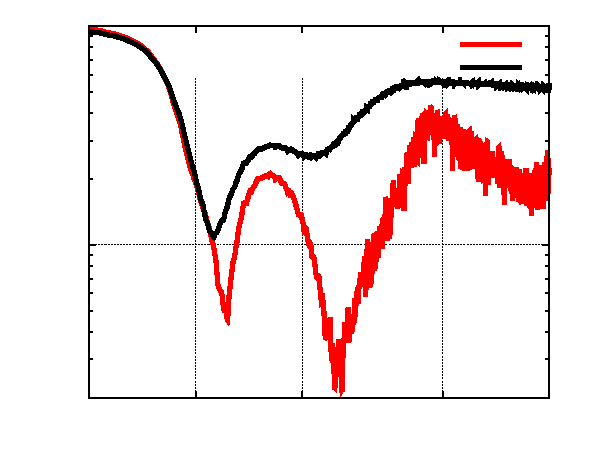
\includegraphics{CaelyxIodixanolIsopoint}}%
    \gplfronttext
  \end{picture}%
\endgroup
}\label{fig:CaelyxIodixanolIsopoint}}
		\caption{ a) Scattering curves at different suspending medium electron densities obtained with a solvent density gradient of Caelyx in aqueous iodixanol with constant buffer osmolality. Figure b) shows the precise position of the isoscattering points before and after the proper correction of the backbround.}
\end{figure}

The solvent background has been subtracted by measuring the scattering curves of a density gradient of Optiprep$\textregistered$ and buffer without nanocarriers. The low scattering power of the PEGylated liposomal doxorubicin at high $q$ values and the contribution of the iodixanol background result in an increased uncertainty in the high-$q$ range of the corrected scattering curves, although in the Fourier region below $q = 0.3$ nm$^{-1}$ the background effect is much less dominant.

\subsection{Isoscattering point approach}
In the low $q$ part of the scattering curve, an isoscattering point is clearly visible as highlighted in figure \ref{fig:CaelyxIodixanolContinuousSAXS}, where all the scattering curves intersect at one point. The isoscattering point position relates directly to the external radius of the measured particle inaccessible to the solvent, as explained in the \textcolor{red}{Supplementary Information.  WHERE?}. Therefore, the PEG-chains attached to the liposome surface might not be quantified in this approach due to the permeability of the polymer layer. The isoscattering point position is precisely determined by calculating the relative standard deviation of all the scattering curves at each $q$-value, as shown in figure \ref{fig:CaelyxIodixanolIsopoint}. \textcolor{blue}{As discussed before \textcolor{red}{WHERE????}, the proper subtraction of the solvent background is essential for the right interpretation of the data, specially for intense incoherent scatterers like Optiprep $\textregistered$. A clear shift in the minima of the relative standard deviation curve is observed in figure \ref{fig:CaelyxIodixanolIsopoint} after correcting the background effects.} Hence, the first isoscattering point $q^{\star}_1$ is located at $q^{\star}_1 = 0.123$ nm$^{-1}$, which corresponds to a radius of $R = 36.5$ nm and a diameter of 73 nm. A second isoscattering point at $q^{\star}_2 = 0.25$ nm$^{-1}$ is still visible, although the diffuseness of the isoscattering points at higher $q$ values, related with the polydispersity of the ensemble, makes it less reliable for the determination of the outer radius.

The determination of the $q$ values have an associated relative uncertainty of 0.1 $\%$, which corresponds to a size uncertainty of 0.6 nm. Furthermore, the radial integration of the scattering pattern was performed choosing a $q$-bin of size 0.0015 nm$^{-1}$, with an associated uncertainty in the size of 0.9 nm. Without further considerations, the Caelyx$\textregistered$ size uncertainty associated to the determination of the $q$-value of the isoscattering point is 1.1 nm. Other possible sources of uncertainty arise from the polydispersity degree of the sample and the ellipticity of the doxorubicin loaded liposomes, which might shift the measured position of the isoscattering point, although the uncertainty associated to them cannot be easily quantified. 

\subsection{Shape factor calculation}
In order to provide a traceable uncertainty for the obtained size value, we have used an alternative evaluation procedure, namely the calculation of the so-called shape factor \citep{stuhrmann_elimination_1965, stuhrmann_elimination_1967} which extracts all contributions from the 30 measured scattering curves that change with the contrast at different solvent densities. The shape factor of the Caelyx$\textregistered$ sample contains essentially information only about the shape and size distribution of the space filled up by the liposomes, i.e. the contributions of the phospholipid bilayer and the encapsulated doxorubicin to the scattering intensity are cancelled.  Thus, the complex interpretation of the original SAXS curve of Caelyx$\textregistered$ is avoided and enables the size determination of the liposomal carrier by fitting a simple analytical model for homogeneous spherical objects. A model with a certain ellipticity was also attempted, due to the slight liposomal eccentricity observed in TEM images \citep{barenholz_doxil_2012} though the best fit was accomplished with a spherical model. Details on the calculation of the shape factor as well as the analytical expression for the model fitting can be found in the \textcolor{red}{Supplementary Information.  WHERE?}. 

\begin{figure}
	\centering
		% GNUPLOT: LaTeX picture with Postscript
\begingroup
  \makeatletter
  \providecommand\color[2][]{%
    \GenericError{(gnuplot) \space\space\space\@spaces}{%
      Package color not loaded in conjunction with
      terminal option `colourtext'%
    }{See the gnuplot documentation for explanation.%
    }{Either use 'blacktext' in gnuplot or load the package
      color.sty in LaTeX.}%
    \renewcommand\color[2][]{}%
  }%
  \providecommand\includegraphics[2][]{%
    \GenericError{(gnuplot) \space\space\space\@spaces}{%
      Package graphicx or graphics not loaded%
    }{See the gnuplot documentation for explanation.%
    }{The gnuplot epslatex terminal needs graphicx.sty or graphics.sty.}%
    \renewcommand\includegraphics[2][]{}%
  }%
  \providecommand\rotatebox[2]{#2}%
  \@ifundefined{ifGPcolor}{%
    \newif\ifGPcolor
    \GPcolortrue
  }{}%
  \@ifundefined{ifGPblacktext}{%
    \newif\ifGPblacktext
    \GPblacktextfalse
  }{}%
  % define a \g@addto@macro without @ in the name:
  \let\gplgaddtomacro\g@addto@macro
  % define empty templates for all commands taking text:
  \gdef\gplbacktext{}%
  \gdef\gplfronttext{}%
  \makeatother
  \ifGPblacktext
    % no textcolor at all
    \def\colorrgb#1{}%
    \def\colorgray#1{}%
  \else
    % gray or color?
    \ifGPcolor
      \def\colorrgb#1{\color[rgb]{#1}}%
      \def\colorgray#1{\color[gray]{#1}}%
      \expandafter\def\csname LTw\endcsname{\color{white}}%
      \expandafter\def\csname LTb\endcsname{\color{black}}%
      \expandafter\def\csname LTa\endcsname{\color{black}}%
      \expandafter\def\csname LT0\endcsname{\color[rgb]{1,0,0}}%
      \expandafter\def\csname LT1\endcsname{\color[rgb]{0,1,0}}%
      \expandafter\def\csname LT2\endcsname{\color[rgb]{0,0,1}}%
      \expandafter\def\csname LT3\endcsname{\color[rgb]{1,0,1}}%
      \expandafter\def\csname LT4\endcsname{\color[rgb]{0,1,1}}%
      \expandafter\def\csname LT5\endcsname{\color[rgb]{1,1,0}}%
      \expandafter\def\csname LT6\endcsname{\color[rgb]{0,0,0}}%
      \expandafter\def\csname LT7\endcsname{\color[rgb]{1,0.3,0}}%
      \expandafter\def\csname LT8\endcsname{\color[rgb]{0.5,0.5,0.5}}%
    \else
      % gray
      \def\colorrgb#1{\color{black}}%
      \def\colorgray#1{\color[gray]{#1}}%
      \expandafter\def\csname LTw\endcsname{\color{white}}%
      \expandafter\def\csname LTb\endcsname{\color{black}}%
      \expandafter\def\csname LTa\endcsname{\color{black}}%
      \expandafter\def\csname LT0\endcsname{\color{black}}%
      \expandafter\def\csname LT1\endcsname{\color{black}}%
      \expandafter\def\csname LT2\endcsname{\color{black}}%
      \expandafter\def\csname LT3\endcsname{\color{black}}%
      \expandafter\def\csname LT4\endcsname{\color{black}}%
      \expandafter\def\csname LT5\endcsname{\color{black}}%
      \expandafter\def\csname LT6\endcsname{\color{black}}%
      \expandafter\def\csname LT7\endcsname{\color{black}}%
      \expandafter\def\csname LT8\endcsname{\color{black}}%
    \fi
  \fi
  \setlength{\unitlength}{0.0500bp}%
  \begin{picture}(5668.00,4534.00)%
    \gplgaddtomacro\gplbacktext{%
      \csname LTb\endcsname%
      \put(990,704){\makebox(0,0)[r]{\strut{} 1}}%
      \csname LTb\endcsname%
      \put(990,1595){\makebox(0,0)[r]{\strut{} 10}}%
      \csname LTb\endcsname%
      \put(990,2487){\makebox(0,0)[r]{\strut{} 100}}%
      \csname LTb\endcsname%
      \put(990,3378){\makebox(0,0)[r]{\strut{} 1000}}%
      \csname LTb\endcsname%
      \put(990,4269){\makebox(0,0)[r]{\strut{} 10000}}%
      \csname LTb\endcsname%
      \put(2279,484){\makebox(0,0){\strut{} 0.05}}%
      \csname LTb\endcsname%
      \put(3437,484){\makebox(0,0){\strut{} 0.1}}%
      \csname LTb\endcsname%
      \put(4594,484){\makebox(0,0){\strut{} 0.2}}%
      \csname LTb\endcsname%
      \put(5271,484){\makebox(0,0){\strut{} 0.3}}%
      \put(220,2486){\rotatebox{-270}{\makebox(0,0){\strut{}Shape Factor / a.u.}}}%
      \put(3196,154){\makebox(0,0){\strut{}$q$ / nm$^{-1}$}}%
    }%
    \gplgaddtomacro\gplfronttext{%
      \csname LTb\endcsname%
      \put(4284,4010){\makebox(0,0)[r]{\strut{}Experimental Data}}%
      \csname LTb\endcsname%
      \put(4284,3617){\makebox(0,0)[r]{\strut{}Sphere Fit}}%
    }%
    \gplbacktext
    \put(0,0){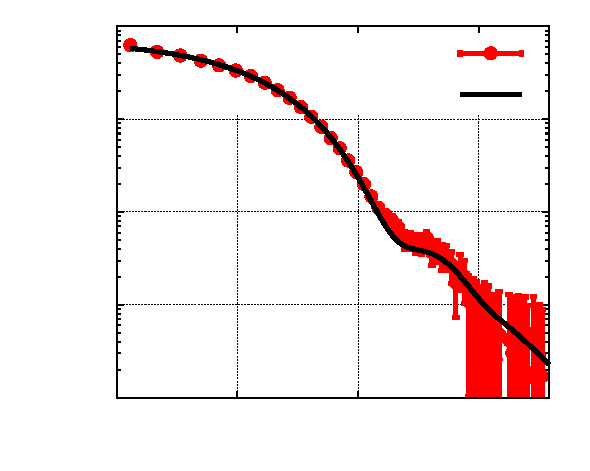
\includegraphics{CaelyxIodixanolResonantTerm}}%
    \gplfronttext
  \end{picture}%
\endgroup

		\caption{Expeirmental shape factor of the liposomes is shown with symbols and the model fit for homogeneous spherical particles is depicted with a thick line.}
		\label{fig:CaelyxIodixanolResonantTerm}
\end{figure}

The shape factor calculated from the SAXS curves and the theoretical model fitting are depicted in figure \ref{fig:CaelyxIodixanolResonantTerm}. The mean diameter obtained from the spherical form factor fit is (65.5 $\pm$ 4.7) nm, slightly smaller than the value calculated from the isoscattering point position. Nevertheless, both values overlap when considering the associated standard uncertainties and that the polydispersity smearing of the isoscattering point is difficult to quantify. The latter fact is supported by the broad size distribution determined by the shape factor fitting. When assuming a Gaussian size distribution, the polydispersity degree (defined as the full width at half maximum of the size distribution divided by its mean value) of the nanocarrier is ca. 40$\%$. Therefore, the average value of (69 $\pm$ 5) nm can be embraced as a reliable external size for the liposomal drug-carrier.

The average size obtained by contrast variation in SAXS is smaller than the result obtained with DLS of ca. 86 nm (in-house measurement), which can be attributed to the fact that the DLS measurand is the hydrodynamic size of the nanoparticles, while SAXS provides the size of the spherical volume inaccessible to the solvent. As the 2 kDa PEG-chains attached to the surface of the liposomes contribute to the hydrodynamic radius but that layer is permeable to the solvent and, therefore, invisible to contrast variation SAXS, the ca. 15 nm difference between the sizes determined by DLS and SAXS is justified. 

\subsection{Average electron density}
At low $q$-values, the Guinier approximation can be used as explained in the \textcolor{red}{Supplementary Information.  WHERE?}. By fitting the spherical form factor to the $q$-range just below the first minimum of the scattering curves, an extrapolated value for the intensity at zero-angle $I(0)$ could be obtained as displayed in figure \ref{fig:CaelyxAverageDensity}. The minimum of the parabola fitted to the experimental points determines the average electron density of the drug carrier system, according to the equation $I(0) \propto (\rho_0-\rho_{solv})^2$  \textcolor{red}{CITE ORIGINAL EQUATION IN THE THESIS - THEORY CHAPTER}.

\begin{figure}
	\centering
		% GNUPLOT: LaTeX picture with Postscript
\begingroup
  \makeatletter
  \providecommand\color[2][]{%
    \GenericError{(gnuplot) \space\space\space\@spaces}{%
      Package color not loaded in conjunction with
      terminal option `colourtext'%
    }{See the gnuplot documentation for explanation.%
    }{Either use 'blacktext' in gnuplot or load the package
      color.sty in LaTeX.}%
    \renewcommand\color[2][]{}%
  }%
  \providecommand\includegraphics[2][]{%
    \GenericError{(gnuplot) \space\space\space\@spaces}{%
      Package graphicx or graphics not loaded%
    }{See the gnuplot documentation for explanation.%
    }{The gnuplot epslatex terminal needs graphicx.sty or graphics.sty.}%
    \renewcommand\includegraphics[2][]{}%
  }%
  \providecommand\rotatebox[2]{#2}%
  \@ifundefined{ifGPcolor}{%
    \newif\ifGPcolor
    \GPcolortrue
  }{}%
  \@ifundefined{ifGPblacktext}{%
    \newif\ifGPblacktext
    \GPblacktextfalse
  }{}%
  % define a \g@addto@macro without @ in the name:
  \let\gplgaddtomacro\g@addto@macro
  % define empty templates for all commands taking text:
  \gdef\gplbacktext{}%
  \gdef\gplfronttext{}%
  \makeatother
  \ifGPblacktext
    % no textcolor at all
    \def\colorrgb#1{}%
    \def\colorgray#1{}%
  \else
    % gray or color?
    \ifGPcolor
      \def\colorrgb#1{\color[rgb]{#1}}%
      \def\colorgray#1{\color[gray]{#1}}%
      \expandafter\def\csname LTw\endcsname{\color{white}}%
      \expandafter\def\csname LTb\endcsname{\color{black}}%
      \expandafter\def\csname LTa\endcsname{\color{black}}%
      \expandafter\def\csname LT0\endcsname{\color[rgb]{1,0,0}}%
      \expandafter\def\csname LT1\endcsname{\color[rgb]{0,1,0}}%
      \expandafter\def\csname LT2\endcsname{\color[rgb]{0,0,1}}%
      \expandafter\def\csname LT3\endcsname{\color[rgb]{1,0,1}}%
      \expandafter\def\csname LT4\endcsname{\color[rgb]{0,1,1}}%
      \expandafter\def\csname LT5\endcsname{\color[rgb]{1,1,0}}%
      \expandafter\def\csname LT6\endcsname{\color[rgb]{0,0,0}}%
      \expandafter\def\csname LT7\endcsname{\color[rgb]{1,0.3,0}}%
      \expandafter\def\csname LT8\endcsname{\color[rgb]{0.5,0.5,0.5}}%
    \else
      % gray
      \def\colorrgb#1{\color{black}}%
      \def\colorgray#1{\color[gray]{#1}}%
      \expandafter\def\csname LTw\endcsname{\color{white}}%
      \expandafter\def\csname LTb\endcsname{\color{black}}%
      \expandafter\def\csname LTa\endcsname{\color{black}}%
      \expandafter\def\csname LT0\endcsname{\color{black}}%
      \expandafter\def\csname LT1\endcsname{\color{black}}%
      \expandafter\def\csname LT2\endcsname{\color{black}}%
      \expandafter\def\csname LT3\endcsname{\color{black}}%
      \expandafter\def\csname LT4\endcsname{\color{black}}%
      \expandafter\def\csname LT5\endcsname{\color{black}}%
      \expandafter\def\csname LT6\endcsname{\color{black}}%
      \expandafter\def\csname LT7\endcsname{\color{black}}%
      \expandafter\def\csname LT8\endcsname{\color{black}}%
    \fi
  \fi
    \setlength{\unitlength}{0.0500bp}%
    \ifx\gptboxheight\undefined%
      \newlength{\gptboxheight}%
      \newlength{\gptboxwidth}%
      \newsavebox{\gptboxtext}%
    \fi%
    \setlength{\fboxrule}{0.5pt}%
    \setlength{\fboxsep}{1pt}%
\begin{picture}(5668.00,4534.00)%
    \gplgaddtomacro\gplbacktext{%
      \csname LTb\endcsname%
      \put(814,704){\makebox(0,0)[r]{\strut{}$0$}}%
      \csname LTb\endcsname%
      \put(814,1274){\makebox(0,0)[r]{\strut{}$20$}}%
      \csname LTb\endcsname%
      \put(814,1845){\makebox(0,0)[r]{\strut{}$40$}}%
      \csname LTb\endcsname%
      \put(814,2415){\makebox(0,0)[r]{\strut{}$60$}}%
      \csname LTb\endcsname%
      \put(814,2986){\makebox(0,0)[r]{\strut{}$80$}}%
      \csname LTb\endcsname%
      \put(814,3556){\makebox(0,0)[r]{\strut{}$100$}}%
      \csname LTb\endcsname%
      \put(814,4126){\makebox(0,0)[r]{\strut{}$120$}}%
      \csname LTb\endcsname%
      \put(1510,484){\makebox(0,0){\strut{}$345$}}%
      \csname LTb\endcsname%
      \put(2450,484){\makebox(0,0){\strut{}$350$}}%
      \csname LTb\endcsname%
      \put(3391,484){\makebox(0,0){\strut{}$355$}}%
      \csname LTb\endcsname%
      \put(4331,484){\makebox(0,0){\strut{}$360$}}%
      \csname LTb\endcsname%
      \put(5271,484){\makebox(0,0){\strut{}$365$}}%
    }%
    \gplgaddtomacro\gplfronttext{%
      \csname LTb\endcsname%
      \put(176,2486){\rotatebox{-270}{\makebox(0,0){\strut{}$I(0)$ / cm$^{-1}$}}}%
      \put(3108,154){\makebox(0,0){\strut{}Solvent Electron Density / nm$^{-3}$}}%
    }%
    \gplbacktext
    \put(0,0){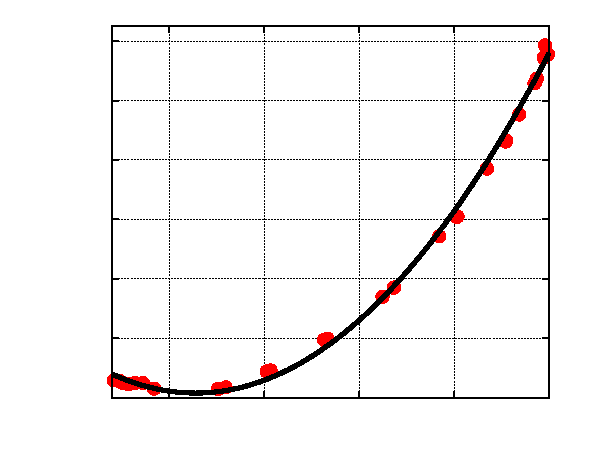
\includegraphics{CaelyxAverageDensity}}%
    \gplfronttext
  \end{picture}%
\endgroup

		\caption{Measured intensity at zero-angle of Caelyx as a function of the electron density of the aqueous iodixanol suspending medium. The function fitted to the experimental data is depicted in black: Average density is 346.39 nm$^{-3}$ and there is a offset of 1.56 cm$^{-1}$}
		\label{fig:CaelyxAverageDensity}
\end{figure}

From this calculation, a value of $\rho_0$ = (346.2 $\pm$ 1.2) nm$^{-3}$ is obtained which corresponds to the density of the liposomal nanocarrier and the precipitated drug combined. The uncertainty of 1.2 nm$^{-3}$ is associated with the vertical size of the focused X-ray beam. The obtained density is slightly higher than the value of 338 nm$^{-3}$ estimated for empty PEGylated liposomes \cite{kucerka_structure_2006} due to the presence of the doxorubicin-sulfate aggregate in the intraliposomal volume.

\section{Osmotic effects in liposomes}

The rigidity of the nanocarriers is a relevant property directly related with its drug delivery efficacy, the particle stability or the release rate of the encapsulated drug. In fact, some of these characteristics might change upon injection due to the osmotic pressure applied to the nanocarriers in the process. In the case of lipid vesicles, i.e. liposomes, the permeability of water through the phopholipid bilayer is a defining aspect of its physicochemical behavior. Although many aspects about the membrane permeability have been studied \cite{nagle_theory_2008, mathai_structural_2008, olbrich_water_2000}, the evaluation of the liposomes rigidity and its osmotic activity is still challenging.

The osmotic behavior of liposomes depends, basically, on their size and chemical composition. For example, the incorporation of cholesterol can vary the fluidity of the lipid bilayer. Larger liposomes tend to be osmotically active \cite{de_gier_osmotic_1993} and behave according to the Laplace law: the osmotic pressure needed to deform them decreases for increasing sizes. In the case of liposomal nanocarriers, the intraliposomal osmolality should be equal to the buffer outside of the liposomes to enhance the particle stability. 

\begin{figure}
	\centering
		% GNUPLOT: LaTeX picture with Postscript
\begingroup
  \makeatletter
  \providecommand\color[2][]{%
    \GenericError{(gnuplot) \space\space\space\@spaces}{%
      Package color not loaded in conjunction with
      terminal option `colourtext'%
    }{See the gnuplot documentation for explanation.%
    }{Either use 'blacktext' in gnuplot or load the package
      color.sty in LaTeX.}%
    \renewcommand\color[2][]{}%
  }%
  \providecommand\includegraphics[2][]{%
    \GenericError{(gnuplot) \space\space\space\@spaces}{%
      Package graphicx or graphics not loaded%
    }{See the gnuplot documentation for explanation.%
    }{The gnuplot epslatex terminal needs graphicx.sty or graphics.sty.}%
    \renewcommand\includegraphics[2][]{}%
  }%
  \providecommand\rotatebox[2]{#2}%
  \@ifundefined{ifGPcolor}{%
    \newif\ifGPcolor
    \GPcolortrue
  }{}%
  \@ifundefined{ifGPblacktext}{%
    \newif\ifGPblacktext
    \GPblacktextfalse
  }{}%
  % define a \g@addto@macro without @ in the name:
  \let\gplgaddtomacro\g@addto@macro
  % define empty templates for all commands taking text:
  \gdef\gplbacktext{}%
  \gdef\gplfronttext{}%
  \makeatother
  \ifGPblacktext
    % no textcolor at all
    \def\colorrgb#1{}%
    \def\colorgray#1{}%
  \else
    % gray or color?
    \ifGPcolor
      \def\colorrgb#1{\color[rgb]{#1}}%
      \def\colorgray#1{\color[gray]{#1}}%
      \expandafter\def\csname LTw\endcsname{\color{white}}%
      \expandafter\def\csname LTb\endcsname{\color{black}}%
      \expandafter\def\csname LTa\endcsname{\color{black}}%
      \expandafter\def\csname LT0\endcsname{\color[rgb]{1,0,0}}%
      \expandafter\def\csname LT1\endcsname{\color[rgb]{0,1,0}}%
      \expandafter\def\csname LT2\endcsname{\color[rgb]{0,0,1}}%
      \expandafter\def\csname LT3\endcsname{\color[rgb]{1,0,1}}%
      \expandafter\def\csname LT4\endcsname{\color[rgb]{0,1,1}}%
      \expandafter\def\csname LT5\endcsname{\color[rgb]{1,1,0}}%
      \expandafter\def\csname LT6\endcsname{\color[rgb]{0,0,0}}%
      \expandafter\def\csname LT7\endcsname{\color[rgb]{1,0.3,0}}%
      \expandafter\def\csname LT8\endcsname{\color[rgb]{0.5,0.5,0.5}}%
    \else
      % gray
      \def\colorrgb#1{\color{black}}%
      \def\colorgray#1{\color[gray]{#1}}%
      \expandafter\def\csname LTw\endcsname{\color{white}}%
      \expandafter\def\csname LTb\endcsname{\color{black}}%
      \expandafter\def\csname LTa\endcsname{\color{black}}%
      \expandafter\def\csname LT0\endcsname{\color{black}}%
      \expandafter\def\csname LT1\endcsname{\color{black}}%
      \expandafter\def\csname LT2\endcsname{\color{black}}%
      \expandafter\def\csname LT3\endcsname{\color{black}}%
      \expandafter\def\csname LT4\endcsname{\color{black}}%
      \expandafter\def\csname LT5\endcsname{\color{black}}%
      \expandafter\def\csname LT6\endcsname{\color{black}}%
      \expandafter\def\csname LT7\endcsname{\color{black}}%
      \expandafter\def\csname LT8\endcsname{\color{black}}%
    \fi
  \fi
  \setlength{\unitlength}{0.0500bp}%
  \begin{picture}(5668.00,4534.00)%
    \gplgaddtomacro\gplbacktext{%
      \csname LTb\endcsname%
      \put(814,1183){\makebox(0,0)[r]{\strut{} 340}}%
      \csname LTb\endcsname%
      \put(814,1885){\makebox(0,0)[r]{\strut{} 350}}%
      \csname LTb\endcsname%
      \put(814,2588){\makebox(0,0)[r]{\strut{} 360}}%
      \csname LTb\endcsname%
      \put(814,3291){\makebox(0,0)[r]{\strut{} 370}}%
      \csname LTb\endcsname%
      \put(814,3994){\makebox(0,0)[r]{\strut{} 380}}%
      \csname LTb\endcsname%
      \put(946,484){\makebox(0,0){\strut{} 0}}%
      \csname LTb\endcsname%
      \put(1377,484){\makebox(0,0){\strut{} 5}}%
      \csname LTb\endcsname%
      \put(1807,484){\makebox(0,0){\strut{} 10}}%
      \csname LTb\endcsname%
      \put(2238,484){\makebox(0,0){\strut{} 15}}%
      \csname LTb\endcsname%
      \put(2668,484){\makebox(0,0){\strut{} 20}}%
      \csname LTb\endcsname%
      \put(3099,484){\makebox(0,0){\strut{} 25}}%
      \csname LTb\endcsname%
      \put(3530,484){\makebox(0,0){\strut{} 30}}%
      \csname LTb\endcsname%
      \put(3960,484){\makebox(0,0){\strut{} 35}}%
      \csname LTb\endcsname%
      \put(4391,484){\makebox(0,0){\strut{} 40}}%
      \put(4523,704){\makebox(0,0)[l]{\strut{}0}}%
      \put(4523,1407){\makebox(0,0)[l]{\strut{}250}}%
      \put(4523,2006){\makebox(0,0)[l]{\strut{}500}}%
      \put(4523,2525){\makebox(0,0)[l]{\strut{}750}}%
      \put(4523,2977){\makebox(0,0)[l]{\strut{}1000}}%
      \put(4523,3375){\makebox(0,0)[l]{\strut{}1250}}%
      \put(4523,3728){\makebox(0,0)[l]{\strut{}1500}}%
      \put(4523,4043){\makebox(0,0)[l]{\strut{}1750}}%
      \put(176,2486){\rotatebox{-270}{\makebox(0,0){\strut{}Electron Density / nm$^{-3}$}}}%
      \put(5160,2486){\rotatebox{270}{\makebox(0,0){\strut{}Osmolality / mOsm kg$^{-1}$}}}%
      \put(2668,154){\makebox(0,0){\strut{}Sucrose Mass Fraction / $\%$}}%
    }%
    \gplgaddtomacro\gplfronttext{%
    }%
    \gplbacktext
    \put(0,0){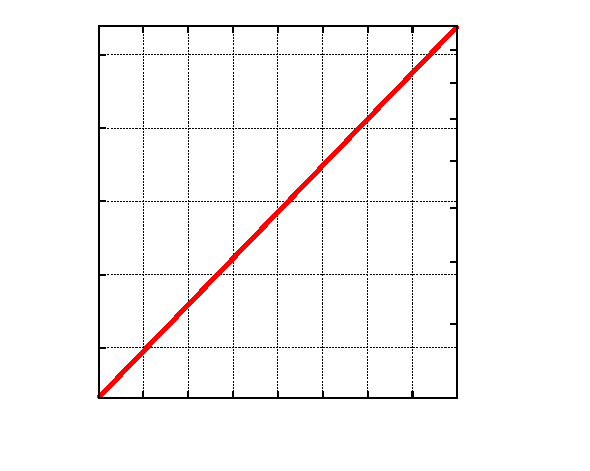
\includegraphics{OsmolalityElectronDensity}}%
    \gplfronttext
  \end{picture}%
\endgroup

		\caption{Relationship between solvent electron density and solvent osmolality for an aqueous sucrose solution.}
		\label{fig:OsmolalityElectronDensity}
\end{figure}

Therefore, it is an important question whether the incorporation of a drug into the intraliposomal volume might modify its osmotic activity. For example, the small size of Caelyx$\textregistered$ and the doxorubicin-sulfate aggregate in the intraliposomal volume create an extraordinary resistance against the buffer osmotic pressure in comparison to the empty liposomal particle. This effect can be studied by increasing systematically the osmolality of the suspending medium by increasing the sucrose concentration in the aqueous buffer. As shown in figure \ref{fig:OsmolalityElectronDensity}, the sucrose molecule acts simultenously as a contrast agent and as an instrument to increase the solvent osmolality. This enables the study of the osmotic effects in liposomes by the denstiy gradient technique with SAXS using aqueous sucrose as suspending medium, as it will be discussed in the following section.

Due to the constant osmolality of the suspending medium along the whole density gradient, no osmotic pressure effects were observed in the size or density of the liposomal drug Caelyx $\textregistered$ in the previous section \ref{sec:caelyx_size}. In this section, a thorough investigation of Caelyx $\textregistered$ under the effects of an increasing solvent osmolality is performed, complementary to the study of the empty liposomal nanocarrier under similar conditions. Besides, the consequences of PEGylation on the liposomal structure are also studied using this technique, focusing principally in its osmotic activity.
 
\subsection{Application to drug-stabilized liposomes}
\label{sec:OsmoticCaelyx}

By means of the density gradient technique, scattering curves of the liposomal doxorubicin were recorded at different sucrose concentrations of the suspending medium, i.e. at different buffer osmolalities, as shown in figure \ref{fig:CaelyxSucroseContinuousSAXS}. The X-ray scattering measurements were performed at two different detector-to-sample distances, as described in section \ref{sec:materials_caelyx}, in order to study a broader $q$-range, spanning from 0.03 to 5.55 nm$^{-1}$, and observe the 1,0-diffraction peak of the doxorubicin fiber-like precipitate around $q=2.3$ nm$^{-1}$ \cite{li_doxorubicin_1998}, as depicted in the figure \ref{fig:CaelyxSucroseContinuousWAXS} after proper background correction.

\begin{figure}
	\centering
		\subfloat[Osmotic effects in Caelyx by using sucrose as contrast agent]{\resizebox{0.44\linewidth}{!}{% GNUPLOT: LaTeX picture with Postscript
\begingroup
  \makeatletter
  \providecommand\color[2][]{%
    \GenericError{(gnuplot) \space\space\space\@spaces}{%
      Package color not loaded in conjunction with
      terminal option `colourtext'%
    }{See the gnuplot documentation for explanation.%
    }{Either use 'blacktext' in gnuplot or load the package
      color.sty in LaTeX.}%
    \renewcommand\color[2][]{}%
  }%
  \providecommand\includegraphics[2][]{%
    \GenericError{(gnuplot) \space\space\space\@spaces}{%
      Package graphicx or graphics not loaded%
    }{See the gnuplot documentation for explanation.%
    }{The gnuplot epslatex terminal needs graphicx.sty or graphics.sty.}%
    \renewcommand\includegraphics[2][]{}%
  }%
  \providecommand\rotatebox[2]{#2}%
  \@ifundefined{ifGPcolor}{%
    \newif\ifGPcolor
    \GPcolortrue
  }{}%
  \@ifundefined{ifGPblacktext}{%
    \newif\ifGPblacktext
    \GPblacktextfalse
  }{}%
  % define a \g@addto@macro without @ in the name:
  \let\gplgaddtomacro\g@addto@macro
  % define empty templates for all commands taking text:
  \gdef\gplbacktext{}%
  \gdef\gplfronttext{}%
  \makeatother
  \ifGPblacktext
    % no textcolor at all
    \def\colorrgb#1{}%
    \def\colorgray#1{}%
  \else
    % gray or color?
    \ifGPcolor
      \def\colorrgb#1{\color[rgb]{#1}}%
      \def\colorgray#1{\color[gray]{#1}}%
      \expandafter\def\csname LTw\endcsname{\color{white}}%
      \expandafter\def\csname LTb\endcsname{\color{black}}%
      \expandafter\def\csname LTa\endcsname{\color{black}}%
      \expandafter\def\csname LT0\endcsname{\color[rgb]{1,0,0}}%
      \expandafter\def\csname LT1\endcsname{\color[rgb]{0,1,0}}%
      \expandafter\def\csname LT2\endcsname{\color[rgb]{0,0,1}}%
      \expandafter\def\csname LT3\endcsname{\color[rgb]{1,0,1}}%
      \expandafter\def\csname LT4\endcsname{\color[rgb]{0,1,1}}%
      \expandafter\def\csname LT5\endcsname{\color[rgb]{1,1,0}}%
      \expandafter\def\csname LT6\endcsname{\color[rgb]{0,0,0}}%
      \expandafter\def\csname LT7\endcsname{\color[rgb]{1,0.3,0}}%
      \expandafter\def\csname LT8\endcsname{\color[rgb]{0.5,0.5,0.5}}%
    \else
      % gray
      \def\colorrgb#1{\color{black}}%
      \def\colorgray#1{\color[gray]{#1}}%
      \expandafter\def\csname LTw\endcsname{\color{white}}%
      \expandafter\def\csname LTb\endcsname{\color{black}}%
      \expandafter\def\csname LTa\endcsname{\color{black}}%
      \expandafter\def\csname LT0\endcsname{\color{black}}%
      \expandafter\def\csname LT1\endcsname{\color{black}}%
      \expandafter\def\csname LT2\endcsname{\color{black}}%
      \expandafter\def\csname LT3\endcsname{\color{black}}%
      \expandafter\def\csname LT4\endcsname{\color{black}}%
      \expandafter\def\csname LT5\endcsname{\color{black}}%
      \expandafter\def\csname LT6\endcsname{\color{black}}%
      \expandafter\def\csname LT7\endcsname{\color{black}}%
      \expandafter\def\csname LT8\endcsname{\color{black}}%
    \fi
  \fi
  \setlength{\unitlength}{0.0500bp}%
  \begin{picture}(5668.00,4534.00)%
    \gplgaddtomacro\gplbacktext{%
      \csname LTb\endcsname%
      \put(814,1053){\makebox(0,0)[r]{\strut{} 0.1}}%
      \csname LTb\endcsname%
      \put(814,2210){\makebox(0,0)[r]{\strut{} 1}}%
      \csname LTb\endcsname%
      \put(814,3368){\makebox(0,0)[r]{\strut{} 10}}%
      \csname LTb\endcsname%
      \put(1434,484){\makebox(0,0){\strut{} 0.05}}%
      \csname LTb\endcsname%
      \put(2096,484){\makebox(0,0){\strut{} 0.1}}%
      \csname LTb\endcsname%
      \put(2758,484){\makebox(0,0){\strut{} 0.2}}%
      \csname LTb\endcsname%
      \put(3633,484){\makebox(0,0){\strut{} 0.5}}%
      \csname LTb\endcsname%
      \put(4295,484){\makebox(0,0){\strut{} 1}}%
      \put(176,2266){\rotatebox{-270}{\makebox(0,0){\strut{}Scattering Intensity / cm$^{-1}$}}}%
      \put(2687,154){\makebox(0,0){\strut{}$q$ / nm$^{-1}$}}%
    }%
    \gplgaddtomacro\gplfronttext{%
      \csname LTb\endcsname%
      \put(4822,778){\makebox(0,0)[l]{\strut{}\smaller 200}}%
      \put(4822,1149){\makebox(0,0)[l]{\strut{}\smaller 400}}%
      \put(4822,1520){\makebox(0,0)[l]{\strut{}\smaller 600}}%
      \put(4822,1892){\makebox(0,0)[l]{\strut{}\smaller 800}}%
      \put(4822,2263){\makebox(0,0)[l]{\strut{}\smaller 1000}}%
      \put(4822,2635){\makebox(0,0)[l]{\strut{}\smaller 1200}}%
      \put(4822,3006){\makebox(0,0)[l]{\strut{}\smaller 1400}}%
      \put(4822,3377){\makebox(0,0)[l]{\strut{}\smaller 1600}}%
      \put(4822,3749){\makebox(0,0)[l]{\strut{}\smaller 1800}}%
      \put(4822,4120){\makebox(0,0)[l]{\strut{}\smaller 2000}}%
      \put(5483,2486){\rotatebox{-90}{\makebox(0,0){\strut{}\smaller Solvent Osmolality / mOsm kg$^{-1}$}}}%
    }%
    \gplbacktext
    \put(0,0){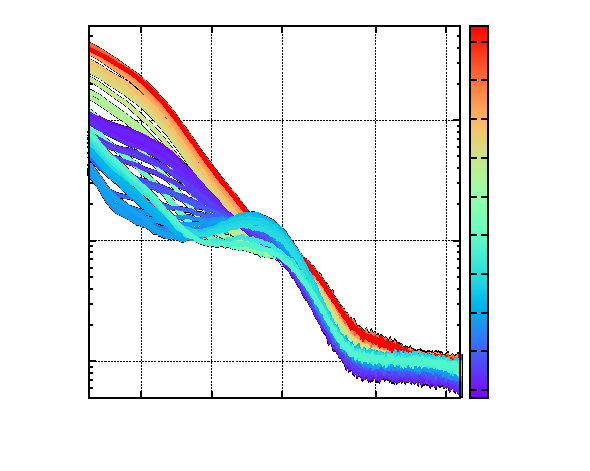
\includegraphics{CaelyxSucroseContinuousSAXS}}%
    \gplfronttext
  \end{picture}%
\endgroup
}\label{fig:CaelyxSucroseContinuousSAXS}}
		\subfloat[Isoscattering point intensity at 2 different setups: Osmotic threshold at 740 mOsm kg$^{-1}$]{\resizebox{0.44\linewidth}{!}{% GNUPLOT: LaTeX picture with Postscript
\begingroup
  \makeatletter
  \providecommand\color[2][]{%
    \GenericError{(gnuplot) \space\space\space\@spaces}{%
      Package color not loaded in conjunction with
      terminal option `colourtext'%
    }{See the gnuplot documentation for explanation.%
    }{Either use 'blacktext' in gnuplot or load the package
      color.sty in LaTeX.}%
    \renewcommand\color[2][]{}%
  }%
  \providecommand\includegraphics[2][]{%
    \GenericError{(gnuplot) \space\space\space\@spaces}{%
      Package graphicx or graphics not loaded%
    }{See the gnuplot documentation for explanation.%
    }{The gnuplot epslatex terminal needs graphicx.sty or graphics.sty.}%
    \renewcommand\includegraphics[2][]{}%
  }%
  \providecommand\rotatebox[2]{#2}%
  \@ifundefined{ifGPcolor}{%
    \newif\ifGPcolor
    \GPcolortrue
  }{}%
  \@ifundefined{ifGPblacktext}{%
    \newif\ifGPblacktext
    \GPblacktextfalse
  }{}%
  % define a \g@addto@macro without @ in the name:
  \let\gplgaddtomacro\g@addto@macro
  % define empty templates for all commands taking text:
  \gdef\gplbacktext{}%
  \gdef\gplfronttext{}%
  \makeatother
  \ifGPblacktext
    % no textcolor at all
    \def\colorrgb#1{}%
    \def\colorgray#1{}%
  \else
    % gray or color?
    \ifGPcolor
      \def\colorrgb#1{\color[rgb]{#1}}%
      \def\colorgray#1{\color[gray]{#1}}%
      \expandafter\def\csname LTw\endcsname{\color{white}}%
      \expandafter\def\csname LTb\endcsname{\color{black}}%
      \expandafter\def\csname LTa\endcsname{\color{black}}%
      \expandafter\def\csname LT0\endcsname{\color[rgb]{1,0,0}}%
      \expandafter\def\csname LT1\endcsname{\color[rgb]{0,1,0}}%
      \expandafter\def\csname LT2\endcsname{\color[rgb]{0,0,1}}%
      \expandafter\def\csname LT3\endcsname{\color[rgb]{1,0,1}}%
      \expandafter\def\csname LT4\endcsname{\color[rgb]{0,1,1}}%
      \expandafter\def\csname LT5\endcsname{\color[rgb]{1,1,0}}%
      \expandafter\def\csname LT6\endcsname{\color[rgb]{0,0,0}}%
      \expandafter\def\csname LT7\endcsname{\color[rgb]{1,0.3,0}}%
      \expandafter\def\csname LT8\endcsname{\color[rgb]{0.5,0.5,0.5}}%
    \else
      % gray
      \def\colorrgb#1{\color{black}}%
      \def\colorgray#1{\color[gray]{#1}}%
      \expandafter\def\csname LTw\endcsname{\color{white}}%
      \expandafter\def\csname LTb\endcsname{\color{black}}%
      \expandafter\def\csname LTa\endcsname{\color{black}}%
      \expandafter\def\csname LT0\endcsname{\color{black}}%
      \expandafter\def\csname LT1\endcsname{\color{black}}%
      \expandafter\def\csname LT2\endcsname{\color{black}}%
      \expandafter\def\csname LT3\endcsname{\color{black}}%
      \expandafter\def\csname LT4\endcsname{\color{black}}%
      \expandafter\def\csname LT5\endcsname{\color{black}}%
      \expandafter\def\csname LT6\endcsname{\color{black}}%
      \expandafter\def\csname LT7\endcsname{\color{black}}%
      \expandafter\def\csname LT8\endcsname{\color{black}}%
    \fi
  \fi
  \setlength{\unitlength}{0.0500bp}%
  \begin{picture}(5668.00,4534.00)%
    \gplgaddtomacro\gplbacktext{%
      \csname LTb\endcsname%
      \put(176,2486){\rotatebox{-270}{\makebox(0,0){\strut{}Intensity at $q=0.123$ nm$^{-1}$ / cm$^{-1}$}}}%
      \put(3108,154){\makebox(0,0){\strut{}Solvent Osmolality / mOsm kg$^{-1}$}}%
    }%
    \gplgaddtomacro\gplfronttext{%
      \csname LTb\endcsname%
      \put(4788,1331){\makebox(0,0)[r]{\strut{}\smaller SAXS}}%
      \csname LTb\endcsname%
      \put(4788,1001){\makebox(0,0)[r]{\strut{}\smaller WAXS}}%
      \csname LTb\endcsname%
      \put(814,704){\makebox(0,0)[r]{\strut{} 0.8}}%
      \csname LTb\endcsname%
      \put(814,1100){\makebox(0,0)[r]{\strut{} 1}}%
      \csname LTb\endcsname%
      \put(814,1496){\makebox(0,0)[r]{\strut{} 1.2}}%
      \csname LTb\endcsname%
      \put(814,1892){\makebox(0,0)[r]{\strut{} 1.4}}%
      \csname LTb\endcsname%
      \put(814,2288){\makebox(0,0)[r]{\strut{} 1.6}}%
      \csname LTb\endcsname%
      \put(814,2685){\makebox(0,0)[r]{\strut{} 1.8}}%
      \csname LTb\endcsname%
      \put(814,3081){\makebox(0,0)[r]{\strut{} 2}}%
      \csname LTb\endcsname%
      \put(814,3477){\makebox(0,0)[r]{\strut{} 2.2}}%
      \csname LTb\endcsname%
      \put(814,3873){\makebox(0,0)[r]{\strut{} 2.4}}%
      \csname LTb\endcsname%
      \put(814,4269){\makebox(0,0)[r]{\strut{} 2.6}}%
      \csname LTb\endcsname%
      \put(1270,484){\makebox(0,0){\strut{} 300}}%
      \csname LTb\endcsname%
      \put(1919,484){\makebox(0,0){\strut{} 600}}%
      \csname LTb\endcsname%
      \put(2568,484){\makebox(0,0){\strut{} 900}}%
      \csname LTb\endcsname%
      \put(3217,484){\makebox(0,0){\strut{} 1200}}%
      \csname LTb\endcsname%
      \put(3865,484){\makebox(0,0){\strut{} 1500}}%
      \csname LTb\endcsname%
      \put(4514,484){\makebox(0,0){\strut{} 1800}}%
      \csname LTb\endcsname%
      \put(5163,484){\makebox(0,0){\strut{} 2100}}%
      \put(2287,3477){\makebox(0,0)[l]{\strut{}\smaller \shortstack{Osmotic\\shrinkage}}}%
      \put(1465,3477){\makebox(0,0){\strut{}\smaller \shortstack{Constant\\shape\\and size}}}%
    }%
    \gplbacktext
    \put(0,0){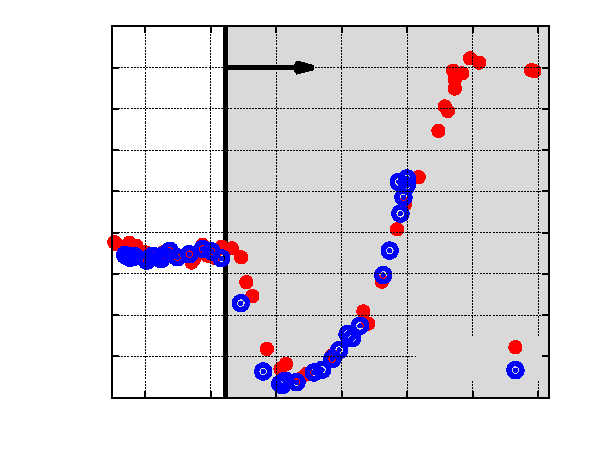
\includegraphics{CaelyxSucroseContinuousSAXSIsopoint}}%
    \gplfronttext
  \end{picture}%
\endgroup
}\label{fig:CaelyxSucroseContinuousSAXSIsopoint}}
		\caption{Scattering curves of Caelyx in an aqueous sucrose density gradient calibrated to the osmolality of the suspending medium. Intensity of the first isoscattering point depending on the aqueous sucrose solution osmolality is shown with black dots.}
\end{figure}

As discussed in the previous section, by increasing the electron density of the suspending medium, the scattering curves of the drug carrier change drastically due to contrast variation. In the case of the aqueous sucrose gradient shown in figure \ref{fig:CaelyxSucroseContinuousSAXS}, this effect is also observed and strongly resembles the curves measured with the Optiprep $\textregistered$ density gradient depicted in figure \ref{fig:CaelyxIodixanolContinuousSAXS}. Nevertheless, upon a certain sucrose concentration (greenish and reddish colored curves in figure \ref{fig:CaelyxSucroseContinuousSAXS}), the features of the scattering curves disappear abruptly, because the suspending medium osmolality is so high that it induces morphological changes in the liposomal structure and, consequently, the scattering form factor of the particles changes.

This effect can be quantified by examining the intensity of the first isoscattering point at $q^{\star}_1 = 0.123$ nm$^{-1}$, because the scattered intensity at this point should be independent of the electron density of the solvent, as observed with the Optiprep $\textregistered$ gradient. The isoscattering point intensity as a function of the suspending medium osmolality is shown in figure \ref{fig:CaelyxSucroseContinuousSAXSIsopoint} and there is a clear osmolality threshold at 670 mOsm kg$^{-1}$. Above this threshold, the osmotic pressure at the liposomal bilayer is so high that the liposome starts shrinking and changes its size, structure and, consequently, scattering form factor. The increased resistance against osmotic pressure, more than double the blood plasma osmolality and much higher than the osmolality needed to shrink empty PEGylated liposomes \cite{varga_osmotic_2014}, is explained by the encapsulation of doxorubicin inside the liposome.

The large osmotic pressure produces a reversible shrinkage of the liposome though it is not capable of cracking it. This was proved in an additional experiment by increasing the osmolality of the buffer to 1333.6 mOsm kg$^{-1}$ with a sucrose mass fraction of 31.4$\%$ and then reducing it to 565.4 mOsm kg-1 by adding distilled water. The solvent with high osmolality produced a featureless scattering curve, as expected from figure \ref{fig:CaelyxSucroseContinuousSAXS}, whereas, after reducing the osmotic pressure, the scattering curve was the same as the measured Caelyx$\textregistered$ curve with the corresponding electron density, which gives evidence that the osmotic shrinkage process is reversible.

\begin{figure}
	\centering
		\subfloat[Osmotic effects in Caelyx by using sucrose as contrast agent]{\resizebox{0.44\linewidth}{!}{% GNUPLOT: LaTeX picture with Postscript
\begingroup
  \makeatletter
  \providecommand\color[2][]{%
    \GenericError{(gnuplot) \space\space\space\@spaces}{%
      Package color not loaded in conjunction with
      terminal option `colourtext'%
    }{See the gnuplot documentation for explanation.%
    }{Either use 'blacktext' in gnuplot or load the package
      color.sty in LaTeX.}%
    \renewcommand\color[2][]{}%
  }%
  \providecommand\includegraphics[2][]{%
    \GenericError{(gnuplot) \space\space\space\@spaces}{%
      Package graphicx or graphics not loaded%
    }{See the gnuplot documentation for explanation.%
    }{The gnuplot epslatex terminal needs graphicx.sty or graphics.sty.}%
    \renewcommand\includegraphics[2][]{}%
  }%
  \providecommand\rotatebox[2]{#2}%
  \@ifundefined{ifGPcolor}{%
    \newif\ifGPcolor
    \GPcolortrue
  }{}%
  \@ifundefined{ifGPblacktext}{%
    \newif\ifGPblacktext
    \GPblacktextfalse
  }{}%
  % define a \g@addto@macro without @ in the name:
  \let\gplgaddtomacro\g@addto@macro
  % define empty templates for all commands taking text:
  \gdef\gplbacktext{}%
  \gdef\gplfronttext{}%
  \makeatother
  \ifGPblacktext
    % no textcolor at all
    \def\colorrgb#1{}%
    \def\colorgray#1{}%
  \else
    % gray or color?
    \ifGPcolor
      \def\colorrgb#1{\color[rgb]{#1}}%
      \def\colorgray#1{\color[gray]{#1}}%
      \expandafter\def\csname LTw\endcsname{\color{white}}%
      \expandafter\def\csname LTb\endcsname{\color{black}}%
      \expandafter\def\csname LTa\endcsname{\color{black}}%
      \expandafter\def\csname LT0\endcsname{\color[rgb]{1,0,0}}%
      \expandafter\def\csname LT1\endcsname{\color[rgb]{0,1,0}}%
      \expandafter\def\csname LT2\endcsname{\color[rgb]{0,0,1}}%
      \expandafter\def\csname LT3\endcsname{\color[rgb]{1,0,1}}%
      \expandafter\def\csname LT4\endcsname{\color[rgb]{0,1,1}}%
      \expandafter\def\csname LT5\endcsname{\color[rgb]{1,1,0}}%
      \expandafter\def\csname LT6\endcsname{\color[rgb]{0,0,0}}%
      \expandafter\def\csname LT7\endcsname{\color[rgb]{1,0.3,0}}%
      \expandafter\def\csname LT8\endcsname{\color[rgb]{0.5,0.5,0.5}}%
    \else
      % gray
      \def\colorrgb#1{\color{black}}%
      \def\colorgray#1{\color[gray]{#1}}%
      \expandafter\def\csname LTw\endcsname{\color{white}}%
      \expandafter\def\csname LTb\endcsname{\color{black}}%
      \expandafter\def\csname LTa\endcsname{\color{black}}%
      \expandafter\def\csname LT0\endcsname{\color{black}}%
      \expandafter\def\csname LT1\endcsname{\color{black}}%
      \expandafter\def\csname LT2\endcsname{\color{black}}%
      \expandafter\def\csname LT3\endcsname{\color{black}}%
      \expandafter\def\csname LT4\endcsname{\color{black}}%
      \expandafter\def\csname LT5\endcsname{\color{black}}%
      \expandafter\def\csname LT6\endcsname{\color{black}}%
      \expandafter\def\csname LT7\endcsname{\color{black}}%
      \expandafter\def\csname LT8\endcsname{\color{black}}%
    \fi
  \fi
  \setlength{\unitlength}{0.0500bp}%
  \begin{picture}(5668.00,4534.00)%
    \gplgaddtomacro\gplbacktext{%
      \csname LTb\endcsname%
      \put(1122,704){\makebox(0,0)[r]{\strut{} 0}}%
      \csname LTb\endcsname%
      \put(1122,1417){\makebox(0,0)[r]{\strut{} 0.0002}}%
      \csname LTb\endcsname%
      \put(1122,2130){\makebox(0,0)[r]{\strut{} 0.0004}}%
      \csname LTb\endcsname%
      \put(1122,2843){\makebox(0,0)[r]{\strut{} 0.0006}}%
      \csname LTb\endcsname%
      \put(1122,3556){\makebox(0,0)[r]{\strut{} 0.0008}}%
      \csname LTb\endcsname%
      \put(1122,4269){\makebox(0,0)[r]{\strut{} 0.001}}%
      \put(220,2266){\rotatebox{-270}{\makebox(0,0){\strut{}Scattering Intensity / cm$^{-1}$}}}%
      \put(2857,154){\makebox(0,0){\strut{}$q$ / nm$^{-1}$}}%
    }%
    \gplgaddtomacro\gplfronttext{%
      \csname LTb\endcsname%
      \put(4701,704){\makebox(0,0)[l]{\strut{}\fsmedium 200}}%
      \put(4701,1252){\makebox(0,0)[l]{\strut{}\fsmedium 400}}%
      \put(4701,1800){\makebox(0,0)[l]{\strut{}\fsmedium 600}}%
      \put(4701,2349){\makebox(0,0)[l]{\strut{}\fsmedium 800}}%
      \put(4701,2897){\makebox(0,0)[l]{\strut{}\fsmedium 1000}}%
      \put(4701,3446){\makebox(0,0)[l]{\strut{}\fsmedium 1200}}%
      \put(4701,3994){\makebox(0,0)[l]{\strut{}\fsmedium 1400}}%
      \put(5559,2486){\rotatebox{-90}{\makebox(0,0){\strut{}\fsmedium Solvent Osmolality / mOsm kg$^{-1}$}}}%
    }%
    \gplbacktext
    \put(0,0){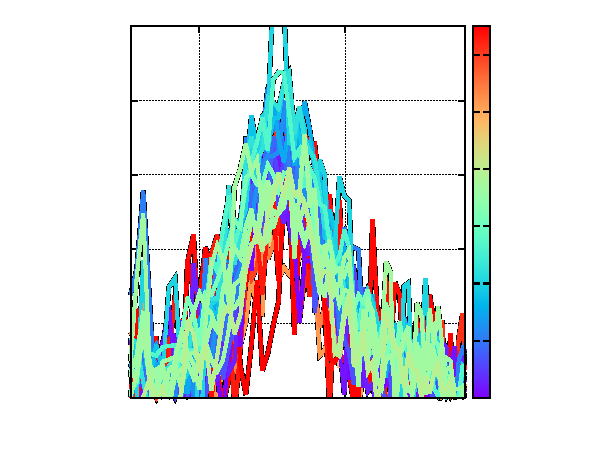
\includegraphics{CaelyxSucroseContinuousWAXS}}%
    \gplfronttext
  \end{picture}%
\endgroup
}\label{fig:CaelyxSucroseContinuousWAXS}}
		\subfloat[Diffraction peak width and position]{\resizebox{0.44\linewidth}{!}{% GNUPLOT: LaTeX picture with Postscript
\begingroup
  \makeatletter
  \providecommand\color[2][]{%
    \GenericError{(gnuplot) \space\space\space\@spaces}{%
      Package color not loaded in conjunction with
      terminal option `colourtext'%
    }{See the gnuplot documentation for explanation.%
    }{Either use 'blacktext' in gnuplot or load the package
      color.sty in LaTeX.}%
    \renewcommand\color[2][]{}%
  }%
  \providecommand\includegraphics[2][]{%
    \GenericError{(gnuplot) \space\space\space\@spaces}{%
      Package graphicx or graphics not loaded%
    }{See the gnuplot documentation for explanation.%
    }{The gnuplot epslatex terminal needs graphicx.sty or graphics.sty.}%
    \renewcommand\includegraphics[2][]{}%
  }%
  \providecommand\rotatebox[2]{#2}%
  \@ifundefined{ifGPcolor}{%
    \newif\ifGPcolor
    \GPcolortrue
  }{}%
  \@ifundefined{ifGPblacktext}{%
    \newif\ifGPblacktext
    \GPblacktextfalse
  }{}%
  % define a \g@addto@macro without @ in the name:
  \let\gplgaddtomacro\g@addto@macro
  % define empty templates for all commands taking text:
  \gdef\gplbacktext{}%
  \gdef\gplfronttext{}%
  \makeatother
  \ifGPblacktext
    % no textcolor at all
    \def\colorrgb#1{}%
    \def\colorgray#1{}%
  \else
    % gray or color?
    \ifGPcolor
      \def\colorrgb#1{\color[rgb]{#1}}%
      \def\colorgray#1{\color[gray]{#1}}%
      \expandafter\def\csname LTw\endcsname{\color{white}}%
      \expandafter\def\csname LTb\endcsname{\color{black}}%
      \expandafter\def\csname LTa\endcsname{\color{black}}%
      \expandafter\def\csname LT0\endcsname{\color[rgb]{1,0,0}}%
      \expandafter\def\csname LT1\endcsname{\color[rgb]{0,1,0}}%
      \expandafter\def\csname LT2\endcsname{\color[rgb]{0,0,1}}%
      \expandafter\def\csname LT3\endcsname{\color[rgb]{1,0,1}}%
      \expandafter\def\csname LT4\endcsname{\color[rgb]{0,1,1}}%
      \expandafter\def\csname LT5\endcsname{\color[rgb]{1,1,0}}%
      \expandafter\def\csname LT6\endcsname{\color[rgb]{0,0,0}}%
      \expandafter\def\csname LT7\endcsname{\color[rgb]{1,0.3,0}}%
      \expandafter\def\csname LT8\endcsname{\color[rgb]{0.5,0.5,0.5}}%
    \else
      % gray
      \def\colorrgb#1{\color{black}}%
      \def\colorgray#1{\color[gray]{#1}}%
      \expandafter\def\csname LTw\endcsname{\color{white}}%
      \expandafter\def\csname LTb\endcsname{\color{black}}%
      \expandafter\def\csname LTa\endcsname{\color{black}}%
      \expandafter\def\csname LT0\endcsname{\color{black}}%
      \expandafter\def\csname LT1\endcsname{\color{black}}%
      \expandafter\def\csname LT2\endcsname{\color{black}}%
      \expandafter\def\csname LT3\endcsname{\color{black}}%
      \expandafter\def\csname LT4\endcsname{\color{black}}%
      \expandafter\def\csname LT5\endcsname{\color{black}}%
      \expandafter\def\csname LT6\endcsname{\color{black}}%
      \expandafter\def\csname LT7\endcsname{\color{black}}%
      \expandafter\def\csname LT8\endcsname{\color{black}}%
    \fi
  \fi
  \setlength{\unitlength}{0.0500bp}%
  \begin{picture}(5668.00,4534.00)%
    \gplgaddtomacro\gplbacktext{%
      \csname LTb\endcsname%
      \put(814,1028){\makebox(0,0)[r]{\strut{}-1}}%
      \csname LTb\endcsname%
      \put(814,1838){\makebox(0,0)[r]{\strut{}-0.5}}%
      \csname LTb\endcsname%
      \put(814,2649){\makebox(0,0)[r]{\strut{} 0}}%
      \csname LTb\endcsname%
      \put(814,3459){\makebox(0,0)[r]{\strut{} 0.5}}%
      \csname LTb\endcsname%
      \put(814,4269){\makebox(0,0)[r]{\strut{} 1}}%
      \csname LTb\endcsname%
      \put(1084,484){\makebox(0,0){\strut{} 250}}%
      \csname LTb\endcsname%
      \put(1922,484){\makebox(0,0){\strut{} 500}}%
      \csname LTb\endcsname%
      \put(2759,484){\makebox(0,0){\strut{} 750}}%
      \csname LTb\endcsname%
      \put(3596,484){\makebox(0,0){\strut{} 1000}}%
      \csname LTb\endcsname%
      \put(4434,484){\makebox(0,0){\strut{} 1250}}%
      \csname LTb\endcsname%
      \put(5271,484){\makebox(0,0){\strut{} 1500}}%
      \put(176,2486){\rotatebox{-270}{\makebox(0,0){\strut{}Diffraction Peak Deviation / $\%$}}}%
      \put(3108,154){\makebox(0,0){\strut{}Solvent Osmolality / mOsm kg$^{-1}$}}%
    }%
    \gplgaddtomacro\gplfronttext{%
    }%
    \gplbacktext
    \put(0,0){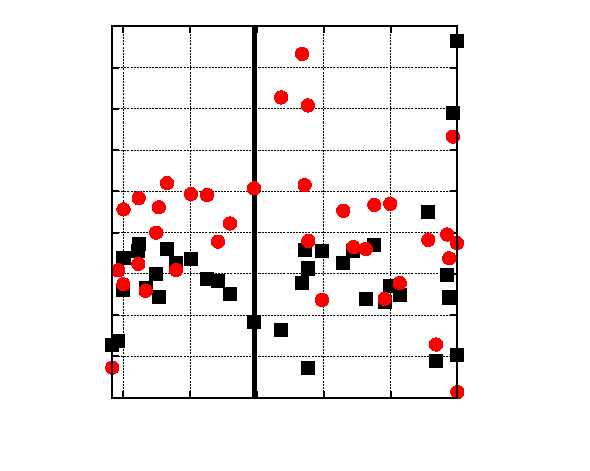
\includegraphics{CaelyxSucroseContinuousWAXSDiffraction}}%
    \gplfronttext
  \end{picture}%
\endgroup
}\label{fig:CaelyxSucroseContinuousWAXSDiffraction}}
		\caption{Measured in WAXS, the $q$-region where the doxorubicin diffraction peak appears can be observed. With black symbols, the shift of the doxorubicin-aggregate diffraction peak from $q=0.123$ nm$^{-1}$ is displayed The mean width (FWHM) is 0.333  nm$^{-1}$}
\end{figure}

The behavior of the nano-drug for an increasing solvent osmolality can be further studied by evaluating the crystal structure of the doxorubicin aggregate, represented by the diffraction peak observed in the figure \ref{fig:CaelyxSucroseContinuousWAXS}. The position of the peak in the reciprocal space depending on the suspending medium osmolality is depicted in figure \ref{fig:CaelyxSucroseContinuousWAXSDiffraction} and shows that its position deviates less than 1 $\%$ from the weighted average $q=2.28$ nm$^{-1}$ along the whole osmolality range. This proves that the fiber-like structure of the drug inside the liposome is also constant during the osmotic shrinkage of the liposomes. The measured position of the (1,0) diffraction peak matches exactly the value measured from doxorubicin-sulfate complexes in solution \cite{lasic_gelation_1992}.\textcolor{blue}{It can also be observed in figure \ref{fig:CaelyxSucroseContinuousWAXSDiffraction} how the width of the diffraction peak does not change sifnificantly along the osmolality range and thus, according to the Scherrer equation \cite{cullity_elements_2001}, the size of the precipated doxorubicin remains stable upon the osmotic shrinkage.}

\begin{figure}
	\centering
		% GNUPLOT: LaTeX picture with Postscript
\begingroup
  \makeatletter
  \providecommand\color[2][]{%
    \GenericError{(gnuplot) \space\space\space\@spaces}{%
      Package color not loaded in conjunction with
      terminal option `colourtext'%
    }{See the gnuplot documentation for explanation.%
    }{Either use 'blacktext' in gnuplot or load the package
      color.sty in LaTeX.}%
    \renewcommand\color[2][]{}%
  }%
  \providecommand\includegraphics[2][]{%
    \GenericError{(gnuplot) \space\space\space\@spaces}{%
      Package graphicx or graphics not loaded%
    }{See the gnuplot documentation for explanation.%
    }{The gnuplot epslatex terminal needs graphicx.sty or graphics.sty.}%
    \renewcommand\includegraphics[2][]{}%
  }%
  \providecommand\rotatebox[2]{#2}%
  \@ifundefined{ifGPcolor}{%
    \newif\ifGPcolor
    \GPcolortrue
  }{}%
  \@ifundefined{ifGPblacktext}{%
    \newif\ifGPblacktext
    \GPblacktextfalse
  }{}%
  % define a \g@addto@macro without @ in the name:
  \let\gplgaddtomacro\g@addto@macro
  % define empty templates for all commands taking text:
  \gdef\gplbacktext{}%
  \gdef\gplfronttext{}%
  \makeatother
  \ifGPblacktext
    % no textcolor at all
    \def\colorrgb#1{}%
    \def\colorgray#1{}%
  \else
    % gray or color?
    \ifGPcolor
      \def\colorrgb#1{\color[rgb]{#1}}%
      \def\colorgray#1{\color[gray]{#1}}%
      \expandafter\def\csname LTw\endcsname{\color{white}}%
      \expandafter\def\csname LTb\endcsname{\color{black}}%
      \expandafter\def\csname LTa\endcsname{\color{black}}%
      \expandafter\def\csname LT0\endcsname{\color[rgb]{1,0,0}}%
      \expandafter\def\csname LT1\endcsname{\color[rgb]{0,1,0}}%
      \expandafter\def\csname LT2\endcsname{\color[rgb]{0,0,1}}%
      \expandafter\def\csname LT3\endcsname{\color[rgb]{1,0,1}}%
      \expandafter\def\csname LT4\endcsname{\color[rgb]{0,1,1}}%
      \expandafter\def\csname LT5\endcsname{\color[rgb]{1,1,0}}%
      \expandafter\def\csname LT6\endcsname{\color[rgb]{0,0,0}}%
      \expandafter\def\csname LT7\endcsname{\color[rgb]{1,0.3,0}}%
      \expandafter\def\csname LT8\endcsname{\color[rgb]{0.5,0.5,0.5}}%
    \else
      % gray
      \def\colorrgb#1{\color{black}}%
      \def\colorgray#1{\color[gray]{#1}}%
      \expandafter\def\csname LTw\endcsname{\color{white}}%
      \expandafter\def\csname LTb\endcsname{\color{black}}%
      \expandafter\def\csname LTa\endcsname{\color{black}}%
      \expandafter\def\csname LT0\endcsname{\color{black}}%
      \expandafter\def\csname LT1\endcsname{\color{black}}%
      \expandafter\def\csname LT2\endcsname{\color{black}}%
      \expandafter\def\csname LT3\endcsname{\color{black}}%
      \expandafter\def\csname LT4\endcsname{\color{black}}%
      \expandafter\def\csname LT5\endcsname{\color{black}}%
      \expandafter\def\csname LT6\endcsname{\color{black}}%
      \expandafter\def\csname LT7\endcsname{\color{black}}%
      \expandafter\def\csname LT8\endcsname{\color{black}}%
    \fi
  \fi
  \setlength{\unitlength}{0.0500bp}%
  \begin{picture}(5668.00,4534.00)%
    \gplgaddtomacro\gplbacktext{%
      \csname LTb\endcsname%
      \put(946,638){\makebox(0,0)[r]{\strut{} 0}}%
      \csname LTb\endcsname%
      \put(946,1243){\makebox(0,0)[r]{\strut{} 0.05}}%
      \csname LTb\endcsname%
      \put(946,1848){\makebox(0,0)[r]{\strut{} 0.1}}%
      \csname LTb\endcsname%
      \put(946,2454){\makebox(0,0)[r]{\strut{} 0.15}}%
      \csname LTb\endcsname%
      \put(946,3059){\makebox(0,0)[r]{\strut{} 0.2}}%
      \csname LTb\endcsname%
      \put(946,3664){\makebox(0,0)[r]{\strut{} 0.25}}%
      \csname LTb\endcsname%
      \put(946,4269){\makebox(0,0)[r]{\strut{} 0.3}}%
      \csname LTb\endcsname%
      \put(1194,418){\makebox(0,0){\strut{} 0.1}}%
      \csname LTb\endcsname%
      \put(2359,418){\makebox(0,0){\strut{} 0.15}}%
      \csname LTb\endcsname%
      \put(3524,418){\makebox(0,0){\strut{} 0.2}}%
      \csname LTb\endcsname%
      \put(4689,418){\makebox(0,0){\strut{} 0.25}}%
      \put(176,2453){\rotatebox{-270}{\makebox(0,0){\strut{}Relative Standard Deviation}}}%
      \put(3174,154){\makebox(0,0){\strut{}$q$ / nm$^{-1}$}}%
    }%
    \gplgaddtomacro\gplfronttext{%
      \csname LTb\endcsname%
      \put(4548,4041){\makebox(0,0)[r]{\strut{}\smaller Optiprep}}%
      \csname LTb\endcsname%
      \put(4548,3711){\makebox(0,0)[r]{\strut{}\smaller Aqueous sucrose}}%
    }%
    \gplbacktext
    \put(0,0){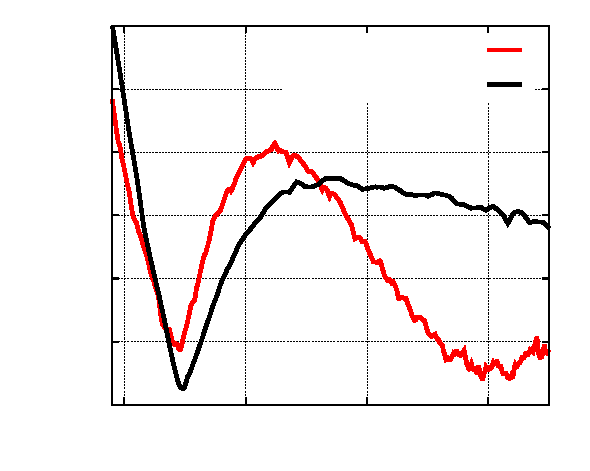
\includegraphics{CaelyxIsopointComparison}}%
    \gplfronttext
  \end{picture}%
\endgroup

		\caption{Isoscattering point position quantified by the calculation of the relative standard deviation of the scattering curves for different solvent density gradients. In the case of the aqueous sucrose solution (black line), only the scattering curves below the osmolality threshold were employed for the calculation.}
		\label{fig:CaelyxIsopointComparison}
\end{figure}

To conclude this section, the diameter obtained from the isoscattering position in the aqueous iodixanol solution can be compared with what is measured in an aqueous sucrose suspending medium. In the latter, if only the scattering curves below this osmolality threshold are considered, the relative standard deviation for each $q$ value reveals a pronounced minimum for the first isoscattering point as depicted in figure \ref{fig:CaelyxIsopointComparison}. When comparing this result with the relative standard deviation curve obtained from the Optiprep $\textregistered$ contrast variation measurements, both values for the size of the drug carrier agree remarkably well within 0.8 $\%$. This reflects the independence of the technique from the contrast agent added to the suspending medium and shows the repeatability of the results.


\subsection{Does PEGylation affect the osmotic activity of liposomes?}
\label{sec:liposome_osmotic}

Typically, unilamellar liposomes present a very narrow size distribution and spherical shape, whose diameter ranges from 50 nm to some hundreds of nanometers, and emerge as suitable nanocarriers for drug delivery. The covalent attachment of biocompatible polymers can improve the liposome stability. For example, polyetyhlene glycol (PEG) shows very low toxicity \cite{yamaoka_distribution_1994} and is a widely used stabilizer \cite{sou_polyethylene_2000}. PEGylated liposomal formulations, also called sterically stabilized liposomes (SSL), show longer blood circulation times \emph{in vivo} \cite{barenholz_liposome_2001} and exhibit a slow drug release rate. PEG-modified liposomes have become of importance lately due to their increased drug pharmakinetics, decreased plasma clearance and improved patient convenience \cite{gabizon_polyethylene_1997,harris_effect_2003}. Therefore, the self-assembly of lipid structures in the presence of PEG moieties has been studied for different lipids \cite{lee_coarse-grained_2011}.

The incorporation of biocompatible polymers increases the phospholipid bilayer strength and enhances the vesicle rigidity, which relates to the increase of the bending modulus \cite{liang_effect_2005, sou_polyethylene_2000}. The higher membrane stiffness of SSLs has been extensively characterized with methods such as Atomic Force Microscopy (AFM) \cite{spyratou_atomic_2009} though other techniques such as light scattering have found a higher osmotic activity in SSLs in comparison to their non-PEGylated counterparts when incubated in serum \cite{wolfram_shrinkage_2014}. Further investigations about the relationship between PEGylation and the liposomal osmotic behavior in suspension are essential. In the following work, the different response of SSLs and plain liposomes to osmotic pressure is studied with SAXS. The creation of multilamellar domains in the phospholipid layer is evaluated and the role of the PEG moieties in the membrane resilience is also analyzed.

\begin{figure}
	\centering
		% GNUPLOT: LaTeX picture with Postscript
\begingroup
  \makeatletter
  \providecommand\color[2][]{%
    \GenericError{(gnuplot) \space\space\space\@spaces}{%
      Package color not loaded in conjunction with
      terminal option `colourtext'%
    }{See the gnuplot documentation for explanation.%
    }{Either use 'blacktext' in gnuplot or load the package
      color.sty in LaTeX.}%
    \renewcommand\color[2][]{}%
  }%
  \providecommand\includegraphics[2][]{%
    \GenericError{(gnuplot) \space\space\space\@spaces}{%
      Package graphicx or graphics not loaded%
    }{See the gnuplot documentation for explanation.%
    }{The gnuplot epslatex terminal needs graphicx.sty or graphics.sty.}%
    \renewcommand\includegraphics[2][]{}%
  }%
  \providecommand\rotatebox[2]{#2}%
  \@ifundefined{ifGPcolor}{%
    \newif\ifGPcolor
    \GPcolortrue
  }{}%
  \@ifundefined{ifGPblacktext}{%
    \newif\ifGPblacktext
    \GPblacktextfalse
  }{}%
  % define a \g@addto@macro without @ in the name:
  \let\gplgaddtomacro\g@addto@macro
  % define empty templates for all commands taking text:
  \gdef\gplbacktext{}%
  \gdef\gplfronttext{}%
  \makeatother
  \ifGPblacktext
    % no textcolor at all
    \def\colorrgb#1{}%
    \def\colorgray#1{}%
  \else
    % gray or color?
    \ifGPcolor
      \def\colorrgb#1{\color[rgb]{#1}}%
      \def\colorgray#1{\color[gray]{#1}}%
      \expandafter\def\csname LTw\endcsname{\color{white}}%
      \expandafter\def\csname LTb\endcsname{\color{black}}%
      \expandafter\def\csname LTa\endcsname{\color{black}}%
      \expandafter\def\csname LT0\endcsname{\color[rgb]{1,0,0}}%
      \expandafter\def\csname LT1\endcsname{\color[rgb]{0,1,0}}%
      \expandafter\def\csname LT2\endcsname{\color[rgb]{0,0,1}}%
      \expandafter\def\csname LT3\endcsname{\color[rgb]{1,0,1}}%
      \expandafter\def\csname LT4\endcsname{\color[rgb]{0,1,1}}%
      \expandafter\def\csname LT5\endcsname{\color[rgb]{1,1,0}}%
      \expandafter\def\csname LT6\endcsname{\color[rgb]{0,0,0}}%
      \expandafter\def\csname LT7\endcsname{\color[rgb]{1,0.3,0}}%
      \expandafter\def\csname LT8\endcsname{\color[rgb]{0.5,0.5,0.5}}%
    \else
      % gray
      \def\colorrgb#1{\color{black}}%
      \def\colorgray#1{\color[gray]{#1}}%
      \expandafter\def\csname LTw\endcsname{\color{white}}%
      \expandafter\def\csname LTb\endcsname{\color{black}}%
      \expandafter\def\csname LTa\endcsname{\color{black}}%
      \expandafter\def\csname LT0\endcsname{\color{black}}%
      \expandafter\def\csname LT1\endcsname{\color{black}}%
      \expandafter\def\csname LT2\endcsname{\color{black}}%
      \expandafter\def\csname LT3\endcsname{\color{black}}%
      \expandafter\def\csname LT4\endcsname{\color{black}}%
      \expandafter\def\csname LT5\endcsname{\color{black}}%
      \expandafter\def\csname LT6\endcsname{\color{black}}%
      \expandafter\def\csname LT7\endcsname{\color{black}}%
      \expandafter\def\csname LT8\endcsname{\color{black}}%
    \fi
  \fi
    \setlength{\unitlength}{0.0500bp}%
    \ifx\gptboxheight\undefined%
      \newlength{\gptboxheight}%
      \newlength{\gptboxwidth}%
      \newsavebox{\gptboxtext}%
    \fi%
    \setlength{\fboxrule}{0.5pt}%
    \setlength{\fboxsep}{1pt}%
\begin{picture}(5668.00,4534.00)%
    \gplgaddtomacro\gplbacktext{%
      \csname LTb\endcsname%
      \put(990,854){\makebox(0,0)[r]{\strut{}$1$}}%
      \csname LTb\endcsname%
      \put(990,1532){\makebox(0,0)[r]{\strut{}$10$}}%
      \csname LTb\endcsname%
      \put(990,2209){\makebox(0,0)[r]{\strut{}$100$}}%
      \csname LTb\endcsname%
      \put(990,2886){\makebox(0,0)[r]{\strut{}$1000$}}%
      \csname LTb\endcsname%
      \put(990,3564){\makebox(0,0)[r]{\strut{}$10000$}}%
      \csname LTb\endcsname%
      \put(990,4241){\makebox(0,0)[r]{\strut{}$100000$}}%
      \csname LTb\endcsname%
      \put(1122,484){\makebox(0,0){\strut{}$0.03$}}%
      \csname LTb\endcsname%
      \put(1706,484){\makebox(0,0){\strut{}$0.05$}}%
      \csname LTb\endcsname%
      \put(2499,484){\makebox(0,0){\strut{}$0.1$}}%
      \csname LTb\endcsname%
      \put(3291,484){\makebox(0,0){\strut{}$0.2$}}%
      \csname LTb\endcsname%
      \put(4339,484){\makebox(0,0){\strut{}$0.5$}}%
      \csname LTb\endcsname%
      \put(5131,484){\makebox(0,0){\strut{}$1$}}%
    }%
    \gplgaddtomacro\gplfronttext{%
      \csname LTb\endcsname%
      \put(220,2266){\rotatebox{-270}{\makebox(0,0){\strut{}Scattering Intensity / a.u.}}}%
      \put(3196,154){\makebox(0,0){\strut{}$q$ / nm$^{-1}$}}%
      \csname LTb\endcsname%
      \put(3015,4098){\makebox(0,0)[r]{\strut{}\smaller PEG 81 nm}}%
      \csname LTb\endcsname%
      \put(3015,3812){\makebox(0,0)[r]{\strut{}\smaller PEG 87 nm}}%
      \csname LTb\endcsname%
      \put(3015,3526){\makebox(0,0)[r]{\strut{}\smaller PEG 103 nm}}%
      \csname LTb\endcsname%
      \put(3015,3240){\makebox(0,0)[r]{\strut{}\smaller PEG 179 nm}}%
      \csname LTb\endcsname%
      \put(4596,4098){\makebox(0,0)[r]{\strut{}\smaller PEG 274 nm}}%
      \csname LTb\endcsname%
      \put(4596,3812){\makebox(0,0)[r]{\strut{}\smaller plain 89 nm}}%
      \csname LTb\endcsname%
      \put(4596,3526){\makebox(0,0)[r]{\strut{}\smaller plain 116 nm}}%
      \csname LTb\endcsname%
      \put(4596,3240){\makebox(0,0)[r]{\strut{}\smaller plain 128 nm}}%
    }%
    \gplbacktext
    \put(0,0){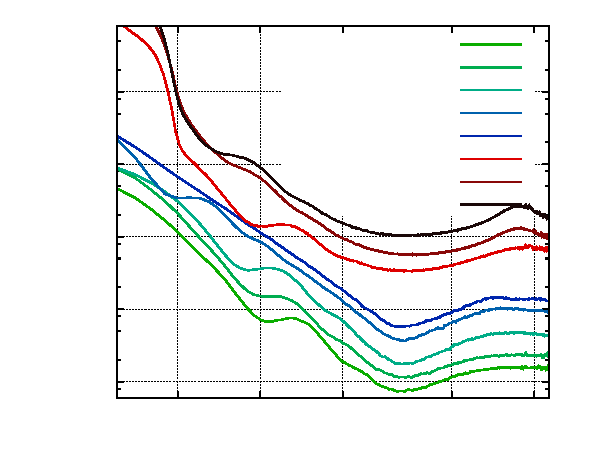
\includegraphics{SSLSingleContrast}}%
    \gplfronttext
  \end{picture}%
\endgroup

		\caption{Scattering curves of the different liposomes in buffer. The curves are intensity shifted for clarity. The 5 SSLs are presented in the lower part of the plot. The sizes in the legend are extracted form DLS measurements.}
		\label{fig:SSLSingleContrast}
\end{figure}

For this purpose, 5 PEGylated and 3 plain liposomes were extruded with different pore sizes, as explained in section \ref{sec:materials_SSL}. To simplify the following discussion, the liposomes are named after the hydrodynamic diameter measured by DLS. The SAXS measurements of the 8 liposomes are showed in figure \ref{fig:SSLSingleContrast}, where the first minimum shifts from $\sim$0.1 nm$^{-1}$ to smaller $q$-values for increasing size. For high polydispersities this scattering minimum gets smeared out, as it can be observed for the 274.1 nm SSL. It can be stated from these measurements and the DLS results that the polydispersity degree rises for increasing liposomal sizes. Besides, non-PEGylated liposomes show slightly broader size distributions than SSLs.

\begin{figure}
	\centering
		% GNUPLOT: LaTeX picture with Postscript
\begingroup
  \makeatletter
  \providecommand\color[2][]{%
    \GenericError{(gnuplot) \space\space\space\@spaces}{%
      Package color not loaded in conjunction with
      terminal option `colourtext'%
    }{See the gnuplot documentation for explanation.%
    }{Either use 'blacktext' in gnuplot or load the package
      color.sty in LaTeX.}%
    \renewcommand\color[2][]{}%
  }%
  \providecommand\includegraphics[2][]{%
    \GenericError{(gnuplot) \space\space\space\@spaces}{%
      Package graphicx or graphics not loaded%
    }{See the gnuplot documentation for explanation.%
    }{The gnuplot epslatex terminal needs graphicx.sty or graphics.sty.}%
    \renewcommand\includegraphics[2][]{}%
  }%
  \providecommand\rotatebox[2]{#2}%
  \@ifundefined{ifGPcolor}{%
    \newif\ifGPcolor
    \GPcolortrue
  }{}%
  \@ifundefined{ifGPblacktext}{%
    \newif\ifGPblacktext
    \GPblacktextfalse
  }{}%
  % define a \g@addto@macro without @ in the name:
  \let\gplgaddtomacro\g@addto@macro
  % define empty templates for all commands taking text:
  \gdef\gplbacktext{}%
  \gdef\gplfronttext{}%
  \makeatother
  \ifGPblacktext
    % no textcolor at all
    \def\colorrgb#1{}%
    \def\colorgray#1{}%
  \else
    % gray or color?
    \ifGPcolor
      \def\colorrgb#1{\color[rgb]{#1}}%
      \def\colorgray#1{\color[gray]{#1}}%
      \expandafter\def\csname LTw\endcsname{\color{white}}%
      \expandafter\def\csname LTb\endcsname{\color{black}}%
      \expandafter\def\csname LTa\endcsname{\color{black}}%
      \expandafter\def\csname LT0\endcsname{\color[rgb]{1,0,0}}%
      \expandafter\def\csname LT1\endcsname{\color[rgb]{0,1,0}}%
      \expandafter\def\csname LT2\endcsname{\color[rgb]{0,0,1}}%
      \expandafter\def\csname LT3\endcsname{\color[rgb]{1,0,1}}%
      \expandafter\def\csname LT4\endcsname{\color[rgb]{0,1,1}}%
      \expandafter\def\csname LT5\endcsname{\color[rgb]{1,1,0}}%
      \expandafter\def\csname LT6\endcsname{\color[rgb]{0,0,0}}%
      \expandafter\def\csname LT7\endcsname{\color[rgb]{1,0.3,0}}%
      \expandafter\def\csname LT8\endcsname{\color[rgb]{0.5,0.5,0.5}}%
    \else
      % gray
      \def\colorrgb#1{\color{black}}%
      \def\colorgray#1{\color[gray]{#1}}%
      \expandafter\def\csname LTw\endcsname{\color{white}}%
      \expandafter\def\csname LTb\endcsname{\color{black}}%
      \expandafter\def\csname LTa\endcsname{\color{black}}%
      \expandafter\def\csname LT0\endcsname{\color{black}}%
      \expandafter\def\csname LT1\endcsname{\color{black}}%
      \expandafter\def\csname LT2\endcsname{\color{black}}%
      \expandafter\def\csname LT3\endcsname{\color{black}}%
      \expandafter\def\csname LT4\endcsname{\color{black}}%
      \expandafter\def\csname LT5\endcsname{\color{black}}%
      \expandafter\def\csname LT6\endcsname{\color{black}}%
      \expandafter\def\csname LT7\endcsname{\color{black}}%
      \expandafter\def\csname LT8\endcsname{\color{black}}%
    \fi
  \fi
  \setlength{\unitlength}{0.0500bp}%
  \begin{picture}(3968.00,6236.00)%
    \gplgaddtomacro\gplbacktext{%
      \csname LTb\endcsname%
      \put(726,1118){\makebox(0,0)[r]{\strut{} 1}}%
      \csname LTb\endcsname%
      \put(726,2983){\makebox(0,0)[r]{\strut{} 10}}%
      \csname LTb\endcsname%
      \put(726,4848){\makebox(0,0)[r]{\strut{} 100}}%
      \csname LTb\endcsname%
      \put(1413,484){\makebox(0,0){\strut{} 0.5}}%
      \csname LTb\endcsname%
      \put(2492,484){\makebox(0,0){\strut{} 1}}%
      \csname LTb\endcsname%
      \put(3571,484){\makebox(0,0){\strut{} 2}}%
      \put(220,3117){\rotatebox{-270}{\makebox(0,0){\strut{}Scattering Intensity / a.u.}}}%
      \put(2214,154){\makebox(0,0){\strut{}$q$ / nm$^{-1}$}}%
    }%
    \gplgaddtomacro\gplfronttext{%
      \csname LTb\endcsname%
      \put(2584,5798){\makebox(0,0)[r]{\strut{}PEG 103 nm}}%
      \csname LTb\endcsname%
      \put(2584,5578){\makebox(0,0)[r]{\strut{}PEG 179 nm}}%
      \csname LTb\endcsname%
      \put(2584,5358){\makebox(0,0)[r]{\strut{}PEG 274 nm}}%
      \csname LTb\endcsname%
      \put(2584,5138){\makebox(0,0)[r]{\strut{}plain 89 nm}}%
      \csname LTb\endcsname%
      \put(2584,4918){\makebox(0,0)[r]{\strut{}plain 128 nm}}%
    }%
    \gplbacktext
    \put(0,0){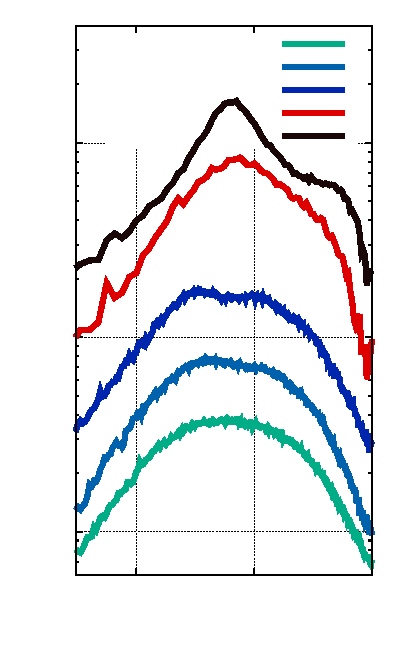
\includegraphics{SSLSingleContrastBilayer}}%
    \gplfronttext
  \end{picture}%
\endgroup

		\caption{The phospholipid bilayer feature: High $q$-region of the scattering curves of 2 plain liposomes and the 3 largest SSLs. The SSLs are presented in the lower part of the plot.}
		\label{fig:SSLSingleContrastBilayer}
\end{figure}

Focusing on the high $q$-region of the single-contrast SAXS curves as displayed in figure \ref{fig:SSLSingleContrastBilayer}, the scattering feature related to the phospholipid bilayer structure is observed. For Unilamellar Vesicles (ULV), the feature shape is typically round with a maximum around $q=0.86$ nm$^{-1}$ \cite{varga_characterization_2012}, related to a distance of 7.3 nm, as it can be seen in the case of small PEGylated liposomes. For SSLs extruded with larger pores, the bilayer shape shows incipient Bragg peaks which suggest the simultaneous presence of Multilamellar Vesicles (MLV) with unilamellar SSLs. Nevertheless, the MLV population cannot exceed 10 $\%$ of the total liposomes \cite{sakuragi_transformation_2011}, as the scattering contribution from ULV is still clearly dominant.

However, the bilayer feature of the plain liposomes differs completely from the round shape visible in unilamellar vesicles. The diffraction peaks appearing at $q_1=0.88$ and $q_2=1.9\simeq2q_1$ nm$^{-1}$ correspond to a slightly smaller lamellar repeat distance of 7.1 nm and the narrow shape of the bilayer feature indicates a variation of the phospholipid bilayer form factor. This change in the bilayer is emphasized for larger vesicles, as observed for the 127.7 plain liposome.

The effect of PEGylation induces a higher membrane stability due to the sterical stabilization of the liposome and the reduction of the electrostatic interactions within the phospholipid bilayer. The electrostatic repulsion in the non-PEGylated membrane is revealed by the appearance of the Bragg peaks in the plain liposomes. Nevertheless, secondary populations of MLVs coexisting with unilamellar liposomes can be observed for large extrusion pore sizes. In conclusion, the size and composition of the liposomes affect remarkably the formation of unilamellar vesicles and the shape of the phospholipid bilayer.

\begin{figure}
	\centering
		% GNUPLOT: LaTeX picture with Postscript
\begingroup
  \makeatletter
  \providecommand\color[2][]{%
    \GenericError{(gnuplot) \space\space\space\@spaces}{%
      Package color not loaded in conjunction with
      terminal option `colourtext'%
    }{See the gnuplot documentation for explanation.%
    }{Either use 'blacktext' in gnuplot or load the package
      color.sty in LaTeX.}%
    \renewcommand\color[2][]{}%
  }%
  \providecommand\includegraphics[2][]{%
    \GenericError{(gnuplot) \space\space\space\@spaces}{%
      Package graphicx or graphics not loaded%
    }{See the gnuplot documentation for explanation.%
    }{The gnuplot epslatex terminal needs graphicx.sty or graphics.sty.}%
    \renewcommand\includegraphics[2][]{}%
  }%
  \providecommand\rotatebox[2]{#2}%
  \@ifundefined{ifGPcolor}{%
    \newif\ifGPcolor
    \GPcolortrue
  }{}%
  \@ifundefined{ifGPblacktext}{%
    \newif\ifGPblacktext
    \GPblacktextfalse
  }{}%
  % define a \g@addto@macro without @ in the name:
  \let\gplgaddtomacro\g@addto@macro
  % define empty templates for all commands taking text:
  \gdef\gplbacktext{}%
  \gdef\gplfronttext{}%
  \makeatother
  \ifGPblacktext
    % no textcolor at all
    \def\colorrgb#1{}%
    \def\colorgray#1{}%
  \else
    % gray or color?
    \ifGPcolor
      \def\colorrgb#1{\color[rgb]{#1}}%
      \def\colorgray#1{\color[gray]{#1}}%
      \expandafter\def\csname LTw\endcsname{\color{white}}%
      \expandafter\def\csname LTb\endcsname{\color{black}}%
      \expandafter\def\csname LTa\endcsname{\color{black}}%
      \expandafter\def\csname LT0\endcsname{\color[rgb]{1,0,0}}%
      \expandafter\def\csname LT1\endcsname{\color[rgb]{0,1,0}}%
      \expandafter\def\csname LT2\endcsname{\color[rgb]{0,0,1}}%
      \expandafter\def\csname LT3\endcsname{\color[rgb]{1,0,1}}%
      \expandafter\def\csname LT4\endcsname{\color[rgb]{0,1,1}}%
      \expandafter\def\csname LT5\endcsname{\color[rgb]{1,1,0}}%
      \expandafter\def\csname LT6\endcsname{\color[rgb]{0,0,0}}%
      \expandafter\def\csname LT7\endcsname{\color[rgb]{1,0.3,0}}%
      \expandafter\def\csname LT8\endcsname{\color[rgb]{0.5,0.5,0.5}}%
    \else
      % gray
      \def\colorrgb#1{\color{black}}%
      \def\colorgray#1{\color[gray]{#1}}%
      \expandafter\def\csname LTw\endcsname{\color{white}}%
      \expandafter\def\csname LTb\endcsname{\color{black}}%
      \expandafter\def\csname LTa\endcsname{\color{black}}%
      \expandafter\def\csname LT0\endcsname{\color{black}}%
      \expandafter\def\csname LT1\endcsname{\color{black}}%
      \expandafter\def\csname LT2\endcsname{\color{black}}%
      \expandafter\def\csname LT3\endcsname{\color{black}}%
      \expandafter\def\csname LT4\endcsname{\color{black}}%
      \expandafter\def\csname LT5\endcsname{\color{black}}%
      \expandafter\def\csname LT6\endcsname{\color{black}}%
      \expandafter\def\csname LT7\endcsname{\color{black}}%
      \expandafter\def\csname LT8\endcsname{\color{black}}%
    \fi
  \fi
  \setlength{\unitlength}{0.0500bp}%
  \begin{picture}(5668.00,4534.00)%
    \gplgaddtomacro\gplbacktext{%
      \csname LTb\endcsname%
      \put(919,967){\makebox(0,0)[r]{\strut{} 1}}%
      \csname LTb\endcsname%
      \put(919,1841){\makebox(0,0)[r]{\strut{} 10}}%
      \csname LTb\endcsname%
      \put(919,2715){\makebox(0,0)[r]{\strut{} 100}}%
      \csname LTb\endcsname%
      \put(919,3589){\makebox(0,0)[r]{\strut{} 1000}}%
      \csname LTb\endcsname%
      \put(1528,484){\makebox(0,0){\strut{} 0.05}}%
      \csname LTb\endcsname%
      \put(2175,484){\makebox(0,0){\strut{} 0.1}}%
      \csname LTb\endcsname%
      \put(2822,484){\makebox(0,0){\strut{} 0.2}}%
      \csname LTb\endcsname%
      \put(3678,484){\makebox(0,0){\strut{} 0.5}}%
      \csname LTb\endcsname%
      \put(4325,484){\makebox(0,0){\strut{} 1}}%
      \put(176,2266){\rotatebox{-270}{\makebox(0,0){\strut{}Scattering Intensity / a.u.}}}%
      \put(2745,154){\makebox(0,0){\strut{}$q$ / nm$^{-1}$}}%
      \colorrgb{0.00,0.00,0.00}%
      \put(1842,1230){\makebox(0,0){\strut{}\smaller \shortstack{Pseudo\\Isoscattering\\Point}}}%
    }%
    \gplgaddtomacro\gplfronttext{%
      \csname LTb\endcsname%
      \put(4825,704){\makebox(0,0)[l]{\strut{}\smaller 0}}%
      \put(4825,1354){\makebox(0,0)[l]{\strut{}\smaller 5}}%
      \put(4825,2005){\makebox(0,0)[l]{\strut{}\smaller 10}}%
      \put(4825,2655){\makebox(0,0)[l]{\strut{}\smaller 15}}%
      \put(4825,3306){\makebox(0,0)[l]{\strut{}\smaller 20}}%
      \put(4825,3956){\makebox(0,0)[l]{\strut{}\smaller 25}}%
      \put(5222,2486){\rotatebox{-90}{\makebox(0,0){\strut{}\smaller Sucrose Mass Fraction / $\%$}}}%
    }%
    \gplbacktext
    \put(0,0){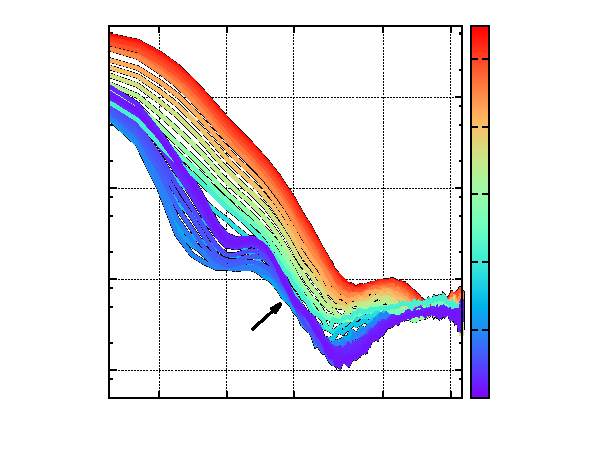
\includegraphics{SSLContinuousSAXS}}%
    \gplfronttext
  \end{picture}%
\endgroup

		\caption{Scattering curves of the 81.4 nm SSL measured at different solvent osmolalities with an aqueous sucrose density gradient. The position of the pseudo isoscattering point at $q=0.18$ nm$^{-1}$ is marked.}
		\label{fig:SSLContinuousSAXS}
\end{figure}

The behavior of the different liposomal structures to osmotic stress can be examined with a continuous contrast variation experiment using sucrose as contrast agent, similarly to the measurements with the Caelyx sample in section \ref{sec:OsmoticCaelyx}. The scattering curves measured for a PEGylated liposome with size 81.4 nm are displayed in figure \ref{fig:SSLContinuousSAXS}, where the solvent osmolality has been increased until 1409 mOsm kg$^{-1}$ using a maximum sucrose mass fraction of 27.3 $\%$. From the low $q$-region of these scattering curves some facts can be extracted which reveal preliminary the structural changes of the liposome induced by the osmotic pressure applied.

\begin{figure}
	\centering
		% GNUPLOT: LaTeX picture with Postscript
\begingroup
  \makeatletter
  \providecommand\color[2][]{%
    \GenericError{(gnuplot) \space\space\space\@spaces}{%
      Package color not loaded in conjunction with
      terminal option `colourtext'%
    }{See the gnuplot documentation for explanation.%
    }{Either use 'blacktext' in gnuplot or load the package
      color.sty in LaTeX.}%
    \renewcommand\color[2][]{}%
  }%
  \providecommand\includegraphics[2][]{%
    \GenericError{(gnuplot) \space\space\space\@spaces}{%
      Package graphicx or graphics not loaded%
    }{See the gnuplot documentation for explanation.%
    }{The gnuplot epslatex terminal needs graphicx.sty or graphics.sty.}%
    \renewcommand\includegraphics[2][]{}%
  }%
  \providecommand\rotatebox[2]{#2}%
  \@ifundefined{ifGPcolor}{%
    \newif\ifGPcolor
    \GPcolortrue
  }{}%
  \@ifundefined{ifGPblacktext}{%
    \newif\ifGPblacktext
    \GPblacktextfalse
  }{}%
  % define a \g@addto@macro without @ in the name:
  \let\gplgaddtomacro\g@addto@macro
  % define empty templates for all commands taking text:
  \gdef\gplbacktext{}%
  \gdef\gplfronttext{}%
  \makeatother
  \ifGPblacktext
    % no textcolor at all
    \def\colorrgb#1{}%
    \def\colorgray#1{}%
  \else
    % gray or color?
    \ifGPcolor
      \def\colorrgb#1{\color[rgb]{#1}}%
      \def\colorgray#1{\color[gray]{#1}}%
      \expandafter\def\csname LTw\endcsname{\color{white}}%
      \expandafter\def\csname LTb\endcsname{\color{black}}%
      \expandafter\def\csname LTa\endcsname{\color{black}}%
      \expandafter\def\csname LT0\endcsname{\color[rgb]{1,0,0}}%
      \expandafter\def\csname LT1\endcsname{\color[rgb]{0,1,0}}%
      \expandafter\def\csname LT2\endcsname{\color[rgb]{0,0,1}}%
      \expandafter\def\csname LT3\endcsname{\color[rgb]{1,0,1}}%
      \expandafter\def\csname LT4\endcsname{\color[rgb]{0,1,1}}%
      \expandafter\def\csname LT5\endcsname{\color[rgb]{1,1,0}}%
      \expandafter\def\csname LT6\endcsname{\color[rgb]{0,0,0}}%
      \expandafter\def\csname LT7\endcsname{\color[rgb]{1,0.3,0}}%
      \expandafter\def\csname LT8\endcsname{\color[rgb]{0.5,0.5,0.5}}%
    \else
      % gray
      \def\colorrgb#1{\color{black}}%
      \def\colorgray#1{\color[gray]{#1}}%
      \expandafter\def\csname LTw\endcsname{\color{white}}%
      \expandafter\def\csname LTb\endcsname{\color{black}}%
      \expandafter\def\csname LTa\endcsname{\color{black}}%
      \expandafter\def\csname LT0\endcsname{\color{black}}%
      \expandafter\def\csname LT1\endcsname{\color{black}}%
      \expandafter\def\csname LT2\endcsname{\color{black}}%
      \expandafter\def\csname LT3\endcsname{\color{black}}%
      \expandafter\def\csname LT4\endcsname{\color{black}}%
      \expandafter\def\csname LT5\endcsname{\color{black}}%
      \expandafter\def\csname LT6\endcsname{\color{black}}%
      \expandafter\def\csname LT7\endcsname{\color{black}}%
      \expandafter\def\csname LT8\endcsname{\color{black}}%
    \fi
  \fi
  \setlength{\unitlength}{0.0500bp}%
  \begin{picture}(5668.00,4534.00)%
    \gplgaddtomacro\gplbacktext{%
      \csname LTb\endcsname%
      \put(550,1088){\makebox(0,0)[r]{\strut{} 0}}%
      \csname LTb\endcsname%
      \put(550,1636){\makebox(0,0)[r]{\strut{} 1}}%
      \csname LTb\endcsname%
      \put(550,2185){\makebox(0,0)[r]{\strut{} 2}}%
      \csname LTb\endcsname%
      \put(550,2733){\makebox(0,0)[r]{\strut{} 3}}%
      \csname LTb\endcsname%
      \put(550,3282){\makebox(0,0)[r]{\strut{} 4}}%
      \csname LTb\endcsname%
      \put(550,3830){\makebox(0,0)[r]{\strut{} 5}}%
      \csname LTb\endcsname%
      \put(682,484){\makebox(0,0){\strut{} 0}}%
      \csname LTb\endcsname%
      \put(1829,484){\makebox(0,0){\strut{} 5}}%
      \csname LTb\endcsname%
      \put(2977,484){\makebox(0,0){\strut{} 10}}%
      \csname LTb\endcsname%
      \put(4124,484){\makebox(0,0){\strut{} 15}}%
      \csname LTb\endcsname%
      \put(5271,484){\makebox(0,0){\strut{} 20}}%
      \put(176,2486){\rotatebox{-270}{\makebox(0,0){\strut{}Deviation from $q^{\star}$ intensity / $\%$}}}%
      \put(2976,154){\makebox(0,0){\strut{}Sucrose Mass Fraction / $\%$}}%
    }%
    \gplgaddtomacro\gplfronttext{%
      \csname LTb\endcsname%
      \put(4284,4096){\makebox(0,0)[r]{\strut{}plain - 89 nm}}%
      \csname LTb\endcsname%
      \put(4284,3876){\makebox(0,0)[r]{\strut{}PEG - 87 nm}}%
    }%
    \gplbacktext
    \put(0,0){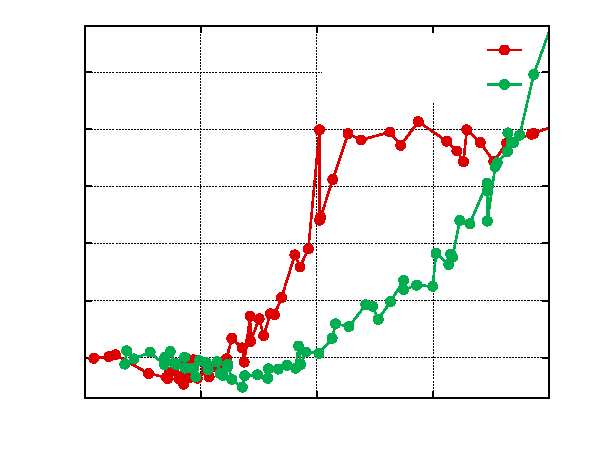
\includegraphics{SSLIsopointIntensity}}%
    \gplfronttext
  \end{picture}%
\endgroup

		\caption{Isoscattering point intensity: Deviation from the initial intensity at $q^{\star}$ at different solvent osmolalities measured for a PEGylated and plain liposome of similar sizes. A clear osmotic threshold can not be observed.}
		\label{fig:SSLIsopointIntensity}
\end{figure}

The curves do not intersect clearly in one point, even for low sucrose concentrations as occured in the Caelyx case. The absence of an evident isoscattering point can be related with the relatively high polydispersity of the sample or the shape variation of the liposome already at small osmotic pressures. However, a diffuse intersection point, or pseudo isoscattering point \cite{kawaguchi_application_2004}, is visible at $q=0.18$ nm$^{-1}$. In analogy to figure \ref{fig:CaelyxSucroseContinuousSAXSIsopoint}, the intensity of the pseudo $q^{\star}$ as a function of the solvent osmolality is depicted in figure \ref{fig:SSLIsopointIntensity}, where the deviation from the original intensity at $q^{\star}$ is shown for a plain and a PEGylated liposome.

The intensity at $q^{\star}$ starts diverging from the original value already at very low solvent osmolalitites and reflects the continuous change in shape or size of the liposome when increasing the osmotic pressure. This behavior occurs for both SSLs and plain liposomes and suggest that a sharp osmotic threshold, like in the Caelyx case, does not exist. Thus, the response of liposomes to osmotic pressure is steady and is already apparent at low osmolalities.

Besides, an evident variaton of the scattering curves below $q\leq0.3$ nm $^{-1}$ is observed in figure \ref{fig:SSLContinuousSAXS} when increasing the solvent osmolality. For example, the minimum originally appearing at 0.1 nm $^{-1}$ shifts slightly to larger $q$-values and dissappears almost completely for high sucrose concentrations. This variation of the form factor is directly related with the flattening of the liposomal shape observed with Freeze-fracture TEM \cite{varga_osmotic_2014}. Due to the increased osmotic activity, the original spherical liposome shrinks into an oblate spheroid. This hypothesis can be further explored by focusing on the scattering feature related to the phospholipid bilayer at the high $q$-region.

\begin{figure}
	\centering
		\subfloat[PEG 178.9 nm]{\resizebox{0.44\linewidth}{!}{% GNUPLOT: LaTeX picture with Postscript
\begingroup
  \makeatletter
  \providecommand\color[2][]{%
    \GenericError{(gnuplot) \space\space\space\@spaces}{%
      Package color not loaded in conjunction with
      terminal option `colourtext'%
    }{See the gnuplot documentation for explanation.%
    }{Either use 'blacktext' in gnuplot or load the package
      color.sty in LaTeX.}%
    \renewcommand\color[2][]{}%
  }%
  \providecommand\includegraphics[2][]{%
    \GenericError{(gnuplot) \space\space\space\@spaces}{%
      Package graphicx or graphics not loaded%
    }{See the gnuplot documentation for explanation.%
    }{The gnuplot epslatex terminal needs graphicx.sty or graphics.sty.}%
    \renewcommand\includegraphics[2][]{}%
  }%
  \providecommand\rotatebox[2]{#2}%
  \@ifundefined{ifGPcolor}{%
    \newif\ifGPcolor
    \GPcolortrue
  }{}%
  \@ifundefined{ifGPblacktext}{%
    \newif\ifGPblacktext
    \GPblacktextfalse
  }{}%
  % define a \g@addto@macro without @ in the name:
  \let\gplgaddtomacro\g@addto@macro
  % define empty templates for all commands taking text:
  \gdef\gplbacktext{}%
  \gdef\gplfronttext{}%
  \makeatother
  \ifGPblacktext
    % no textcolor at all
    \def\colorrgb#1{}%
    \def\colorgray#1{}%
  \else
    % gray or color?
    \ifGPcolor
      \def\colorrgb#1{\color[rgb]{#1}}%
      \def\colorgray#1{\color[gray]{#1}}%
      \expandafter\def\csname LTw\endcsname{\color{white}}%
      \expandafter\def\csname LTb\endcsname{\color{black}}%
      \expandafter\def\csname LTa\endcsname{\color{black}}%
      \expandafter\def\csname LT0\endcsname{\color[rgb]{1,0,0}}%
      \expandafter\def\csname LT1\endcsname{\color[rgb]{0,1,0}}%
      \expandafter\def\csname LT2\endcsname{\color[rgb]{0,0,1}}%
      \expandafter\def\csname LT3\endcsname{\color[rgb]{1,0,1}}%
      \expandafter\def\csname LT4\endcsname{\color[rgb]{0,1,1}}%
      \expandafter\def\csname LT5\endcsname{\color[rgb]{1,1,0}}%
      \expandafter\def\csname LT6\endcsname{\color[rgb]{0,0,0}}%
      \expandafter\def\csname LT7\endcsname{\color[rgb]{1,0.3,0}}%
      \expandafter\def\csname LT8\endcsname{\color[rgb]{0.5,0.5,0.5}}%
    \else
      % gray
      \def\colorrgb#1{\color{black}}%
      \def\colorgray#1{\color[gray]{#1}}%
      \expandafter\def\csname LTw\endcsname{\color{white}}%
      \expandafter\def\csname LTb\endcsname{\color{black}}%
      \expandafter\def\csname LTa\endcsname{\color{black}}%
      \expandafter\def\csname LT0\endcsname{\color{black}}%
      \expandafter\def\csname LT1\endcsname{\color{black}}%
      \expandafter\def\csname LT2\endcsname{\color{black}}%
      \expandafter\def\csname LT3\endcsname{\color{black}}%
      \expandafter\def\csname LT4\endcsname{\color{black}}%
      \expandafter\def\csname LT5\endcsname{\color{black}}%
      \expandafter\def\csname LT6\endcsname{\color{black}}%
      \expandafter\def\csname LT7\endcsname{\color{black}}%
      \expandafter\def\csname LT8\endcsname{\color{black}}%
    \fi
  \fi
  \setlength{\unitlength}{0.0500bp}%
  \begin{picture}(5102.00,10204.00)%
    \gplgaddtomacro\gplbacktext{%
      \csname LTb\endcsname%
      \put(726,1865){\makebox(0,0)[r]{\strut{} 0.2}}%
      \csname LTb\endcsname%
      \put(726,4335){\makebox(0,0)[r]{\strut{} 0.5}}%
      \csname LTb\endcsname%
      \put(726,6203){\makebox(0,0)[r]{\strut{} 1}}%
      \csname LTb\endcsname%
      \put(726,8071){\makebox(0,0)[r]{\strut{} 2}}%
      \csname LTb\endcsname%
      \put(1812,484){\makebox(0,0){\strut{} 0.5}}%
      \csname LTb\endcsname%
      \put(2765,484){\makebox(0,0){\strut{} 1}}%
      \csname LTb\endcsname%
      \put(3719,484){\makebox(0,0){\strut{} 2}}%
      \put(220,5101){\rotatebox{-270}{\makebox(0,0){\strut{}Scattering Intensity / a.u.}}}%
      \put(2384,154){\makebox(0,0){\strut{}$q$ / nm$^{-1}$}}%
    }%
    \gplgaddtomacro\gplfronttext{%
      \csname LTb\endcsname%
      \put(4271,704){\makebox(0,0)[l]{\strut{}\smaller 0}}%
      \put(4271,2463){\makebox(0,0)[l]{\strut{}\smaller 2}}%
      \put(4271,4222){\makebox(0,0)[l]{\strut{}\smaller 4}}%
      \put(4271,5981){\makebox(0,0)[l]{\strut{}\smaller 6}}%
      \put(4271,7740){\makebox(0,0)[l]{\strut{}\smaller 8}}%
      \put(4271,9499){\makebox(0,0)[l]{\strut{}\smaller 10}}%
      \put(4536,5321){\rotatebox{-90}{\makebox(0,0){\strut{}\smaller Sucrose Concentration / $\%$}}}%
    }%
    \gplbacktext
    \put(0,0){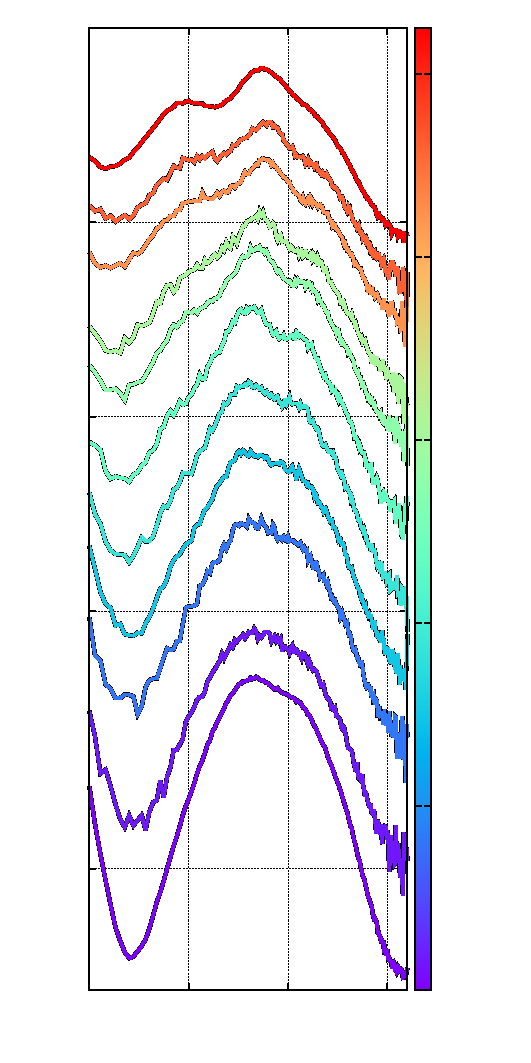
\includegraphics{SSLContrastCurvesBilayer200SSL}}%
    \gplfronttext
  \end{picture}%
\endgroup
}\label{fig:SSLContrastCurvesBilayer200SSL}}
		\subfloat[Plain 127.7 nm]{\resizebox{0.44\linewidth}{!}{% GNUPLOT: LaTeX picture with Postscript
\begingroup
  \makeatletter
  \providecommand\color[2][]{%
    \GenericError{(gnuplot) \space\space\space\@spaces}{%
      Package color not loaded in conjunction with
      terminal option `colourtext'%
    }{See the gnuplot documentation for explanation.%
    }{Either use 'blacktext' in gnuplot or load the package
      color.sty in LaTeX.}%
    \renewcommand\color[2][]{}%
  }%
  \providecommand\includegraphics[2][]{%
    \GenericError{(gnuplot) \space\space\space\@spaces}{%
      Package graphicx or graphics not loaded%
    }{See the gnuplot documentation for explanation.%
    }{The gnuplot epslatex terminal needs graphicx.sty or graphics.sty.}%
    \renewcommand\includegraphics[2][]{}%
  }%
  \providecommand\rotatebox[2]{#2}%
  \@ifundefined{ifGPcolor}{%
    \newif\ifGPcolor
    \GPcolortrue
  }{}%
  \@ifundefined{ifGPblacktext}{%
    \newif\ifGPblacktext
    \GPblacktextfalse
  }{}%
  % define a \g@addto@macro without @ in the name:
  \let\gplgaddtomacro\g@addto@macro
  % define empty templates for all commands taking text:
  \gdef\gplbacktext{}%
  \gdef\gplfronttext{}%
  \makeatother
  \ifGPblacktext
    % no textcolor at all
    \def\colorrgb#1{}%
    \def\colorgray#1{}%
  \else
    % gray or color?
    \ifGPcolor
      \def\colorrgb#1{\color[rgb]{#1}}%
      \def\colorgray#1{\color[gray]{#1}}%
      \expandafter\def\csname LTw\endcsname{\color{white}}%
      \expandafter\def\csname LTb\endcsname{\color{black}}%
      \expandafter\def\csname LTa\endcsname{\color{black}}%
      \expandafter\def\csname LT0\endcsname{\color[rgb]{1,0,0}}%
      \expandafter\def\csname LT1\endcsname{\color[rgb]{0,1,0}}%
      \expandafter\def\csname LT2\endcsname{\color[rgb]{0,0,1}}%
      \expandafter\def\csname LT3\endcsname{\color[rgb]{1,0,1}}%
      \expandafter\def\csname LT4\endcsname{\color[rgb]{0,1,1}}%
      \expandafter\def\csname LT5\endcsname{\color[rgb]{1,1,0}}%
      \expandafter\def\csname LT6\endcsname{\color[rgb]{0,0,0}}%
      \expandafter\def\csname LT7\endcsname{\color[rgb]{1,0.3,0}}%
      \expandafter\def\csname LT8\endcsname{\color[rgb]{0.5,0.5,0.5}}%
    \else
      % gray
      \def\colorrgb#1{\color{black}}%
      \def\colorgray#1{\color[gray]{#1}}%
      \expandafter\def\csname LTw\endcsname{\color{white}}%
      \expandafter\def\csname LTb\endcsname{\color{black}}%
      \expandafter\def\csname LTa\endcsname{\color{black}}%
      \expandafter\def\csname LT0\endcsname{\color{black}}%
      \expandafter\def\csname LT1\endcsname{\color{black}}%
      \expandafter\def\csname LT2\endcsname{\color{black}}%
      \expandafter\def\csname LT3\endcsname{\color{black}}%
      \expandafter\def\csname LT4\endcsname{\color{black}}%
      \expandafter\def\csname LT5\endcsname{\color{black}}%
      \expandafter\def\csname LT6\endcsname{\color{black}}%
      \expandafter\def\csname LT7\endcsname{\color{black}}%
      \expandafter\def\csname LT8\endcsname{\color{black}}%
    \fi
  \fi
    \setlength{\unitlength}{0.0500bp}%
    \ifx\gptboxheight\undefined%
      \newlength{\gptboxheight}%
      \newlength{\gptboxwidth}%
      \newsavebox{\gptboxtext}%
    \fi%
    \setlength{\fboxrule}{0.5pt}%
    \setlength{\fboxsep}{1pt}%
\begin{picture}(3968.00,6236.00)%
    \gplgaddtomacro\gplbacktext{%
      \csname LTb\endcsname%
      \put(594,1199){\makebox(0,0)[r]{\strut{}$1$}}%
      \csname LTb\endcsname%
      \put(594,2843){\makebox(0,0)[r]{\strut{}$10$}}%
      \csname LTb\endcsname%
      \put(594,4486){\makebox(0,0)[r]{\strut{}$100$}}%
      \csname LTb\endcsname%
      \put(1412,484){\makebox(0,0){\strut{}$0.5$}}%
      \csname LTb\endcsname%
      \put(2097,484){\makebox(0,0){\strut{}$1$}}%
      \csname LTb\endcsname%
      \put(2783,484){\makebox(0,0){\strut{}$2$}}%
    }%
    \gplgaddtomacro\gplfronttext{%
      \csname LTb\endcsname%
      \put(220,3117){\rotatebox{-270}{\makebox(0,0){\strut{}Scattering Intensity / a.u.}}}%
      \put(1801,154){\makebox(0,0){\strut{}$q$ / nm$^{-1}$}}%
      \csname LTb\endcsname%
      \put(3170,704){\makebox(0,0)[l]{\strut{}$0$}}%
      \put(3170,1757){\makebox(0,0)[l]{\strut{}$5$}}%
      \put(3170,2810){\makebox(0,0)[l]{\strut{}$10$}}%
      \put(3170,3864){\makebox(0,0)[l]{\strut{}$15$}}%
      \put(3170,4917){\makebox(0,0)[l]{\strut{}$20$}}%
      \put(3170,5971){\makebox(0,0)[l]{\strut{}$25$}}%
      \put(3369,3337){\rotatebox{-90}{\makebox(0,0){\strut{}Sucrose Concentration / $\%$}}}%
    }%
    \gplbacktext
    \put(0,0){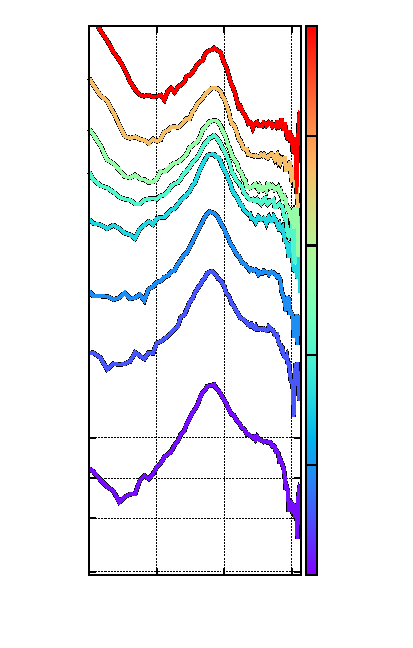
\includegraphics{SSLContrastCurvesBilayer100Plain}}%
    \gplfronttext
  \end{picture}%
\endgroup
}\label{fig:SSLContrastCurvesBilayer100Plain}}
		\caption{Osmotic effects in the phospholipid bilayer: Scattering curves measured at different solvent osmolalities for a 178.9 nm SSL and a 127.7 nm plain liposome. The appearance of Bragg peaks in the SSL membrane contrasts with the unaltered shape of the bilayer in the plain liposome.}
\end{figure}

For this purpose, the bilayer feature of the 178.9 nm PEGylated liposome is shown in figure \ref{fig:SSLContrastCurvesBilayer200SSL} for increasing solvent osmolalities. The scattering curves were measured with sucrose concentrations $\leq10\;\%$ to avoid undesired contrast effects, because the average electron density of the phospholipid bilayer is ca. 348 nm$^{-3}$, which corresponds to a sucrose mass fraction of $\sim 12 \; \%$. Indeed, the bilayer form factor shows undesired, large contrast effects for solvent densities close to the average density of the membrane, i.e. match point, as already observed in figure \ref{fig:SSLContinuousSAXS}, where the bilayer feature shifts abruptly to smaller $q$-values for sucrose concentrations above 15 $\%$. The convolution of the contrast-related effects with the variations induced by the osmotic pressure demands a more challenging evaluation, can prevent the right interpretation of the data and is, thus, unwanted.

The original double-peak structure of the SSL at 0 $\%$ sucrose concentration observed in figure \ref{fig:SSLContrastCurvesBilayer200SSL} transforms upon increasing the solvent osmolality and splits into 3 peaks of decreasing intensity at $q_1=0.48$ nm$^{-1}$, $q_2=0.86$ nm$^{-1}$ and $q_3=1.28$ nm$^{-1}$. These Bragg peaks superimposed on the bilayer form factor reveal a periodic structure which can be related with a partial oligolamellar structure in the liposome system \cite{fernandez_influence_2008}. The 3 mentioned diffraction peaks translate into a lamellar repeat distance of ca. 13 nm, approximately doubling the thickness of the single phospholipid bilayer \cite{kenworthy_range_1995} and suggesting the appearance of a bilamellar structure \cite{deme_giant_2002}. 

The transition between a single bilayer phase and a bilamellar phase at 10 $\%$ sucrose concentration supports the hypothesis already presented that the liposome shrinks into lens-shaped vesicles due to the osmotic pressure. The bilamellar structure might arise from the close bilayer contacts at the outest part of the elliptical liposomes, while the single bilayer conformation still remains dominant in the midsection of the liposomes. A similar morphology has been observed after the osmotic shrinkage of DPPC/DSPE-PEG$_{2000}$ vesicles \cite{terreno_osmotically_2009}. In fact, this behavior was identical for all 5 studied PEGylated liposomes, independent of their size. 

\begin{figure}
	\centering
		% GNUPLOT: LaTeX picture with Postscript
\begingroup
  \makeatletter
  \providecommand\color[2][]{%
    \GenericError{(gnuplot) \space\space\space\@spaces}{%
      Package color not loaded in conjunction with
      terminal option `colourtext'%
    }{See the gnuplot documentation for explanation.%
    }{Either use 'blacktext' in gnuplot or load the package
      color.sty in LaTeX.}%
    \renewcommand\color[2][]{}%
  }%
  \providecommand\includegraphics[2][]{%
    \GenericError{(gnuplot) \space\space\space\@spaces}{%
      Package graphicx or graphics not loaded%
    }{See the gnuplot documentation for explanation.%
    }{The gnuplot epslatex terminal needs graphicx.sty or graphics.sty.}%
    \renewcommand\includegraphics[2][]{}%
  }%
  \providecommand\rotatebox[2]{#2}%
  \@ifundefined{ifGPcolor}{%
    \newif\ifGPcolor
    \GPcolortrue
  }{}%
  \@ifundefined{ifGPblacktext}{%
    \newif\ifGPblacktext
    \GPblacktextfalse
  }{}%
  % define a \g@addto@macro without @ in the name:
  \let\gplgaddtomacro\g@addto@macro
  % define empty templates for all commands taking text:
  \gdef\gplbacktext{}%
  \gdef\gplfronttext{}%
  \makeatother
  \ifGPblacktext
    % no textcolor at all
    \def\colorrgb#1{}%
    \def\colorgray#1{}%
  \else
    % gray or color?
    \ifGPcolor
      \def\colorrgb#1{\color[rgb]{#1}}%
      \def\colorgray#1{\color[gray]{#1}}%
      \expandafter\def\csname LTw\endcsname{\color{white}}%
      \expandafter\def\csname LTb\endcsname{\color{black}}%
      \expandafter\def\csname LTa\endcsname{\color{black}}%
      \expandafter\def\csname LT0\endcsname{\color[rgb]{1,0,0}}%
      \expandafter\def\csname LT1\endcsname{\color[rgb]{0,1,0}}%
      \expandafter\def\csname LT2\endcsname{\color[rgb]{0,0,1}}%
      \expandafter\def\csname LT3\endcsname{\color[rgb]{1,0,1}}%
      \expandafter\def\csname LT4\endcsname{\color[rgb]{0,1,1}}%
      \expandafter\def\csname LT5\endcsname{\color[rgb]{1,1,0}}%
      \expandafter\def\csname LT6\endcsname{\color[rgb]{0,0,0}}%
      \expandafter\def\csname LT7\endcsname{\color[rgb]{1,0.3,0}}%
      \expandafter\def\csname LT8\endcsname{\color[rgb]{0.5,0.5,0.5}}%
    \else
      % gray
      \def\colorrgb#1{\color{black}}%
      \def\colorgray#1{\color[gray]{#1}}%
      \expandafter\def\csname LTw\endcsname{\color{white}}%
      \expandafter\def\csname LTb\endcsname{\color{black}}%
      \expandafter\def\csname LTa\endcsname{\color{black}}%
      \expandafter\def\csname LT0\endcsname{\color{black}}%
      \expandafter\def\csname LT1\endcsname{\color{black}}%
      \expandafter\def\csname LT2\endcsname{\color{black}}%
      \expandafter\def\csname LT3\endcsname{\color{black}}%
      \expandafter\def\csname LT4\endcsname{\color{black}}%
      \expandafter\def\csname LT5\endcsname{\color{black}}%
      \expandafter\def\csname LT6\endcsname{\color{black}}%
      \expandafter\def\csname LT7\endcsname{\color{black}}%
      \expandafter\def\csname LT8\endcsname{\color{black}}%
    \fi
  \fi
    \setlength{\unitlength}{0.0500bp}%
    \ifx\gptboxheight\undefined%
      \newlength{\gptboxheight}%
      \newlength{\gptboxwidth}%
      \newsavebox{\gptboxtext}%
    \fi%
    \setlength{\fboxrule}{0.5pt}%
    \setlength{\fboxsep}{1pt}%
\begin{picture}(5668.00,4534.00)%
    \gplgaddtomacro\gplbacktext{%
      \csname LTb\endcsname%
      \put(462,704){\makebox(0,0)[r]{\strut{}$0$}}%
      \csname LTb\endcsname%
      \put(462,1232){\makebox(0,0)[r]{\strut{}$2$}}%
      \csname LTb\endcsname%
      \put(462,1760){\makebox(0,0)[r]{\strut{}$4$}}%
      \csname LTb\endcsname%
      \put(462,2289){\makebox(0,0)[r]{\strut{}$6$}}%
      \csname LTb\endcsname%
      \put(462,2817){\makebox(0,0)[r]{\strut{}$8$}}%
      \csname LTb\endcsname%
      \put(462,3345){\makebox(0,0)[r]{\strut{}$10$}}%
      \csname LTb\endcsname%
      \put(462,3873){\makebox(0,0)[r]{\strut{}$12$}}%
      \csname LTb\endcsname%
      \put(594,484){\makebox(0,0){\strut{}$0$}}%
      \csname LTb\endcsname%
      \put(1144,484){\makebox(0,0){\strut{}$1$}}%
      \csname LTb\endcsname%
      \put(1694,484){\makebox(0,0){\strut{}$2$}}%
      \csname LTb\endcsname%
      \put(2245,484){\makebox(0,0){\strut{}$3$}}%
      \csname LTb\endcsname%
      \put(2795,484){\makebox(0,0){\strut{}$4$}}%
      \csname LTb\endcsname%
      \put(3345,484){\makebox(0,0){\strut{}$5$}}%
      \csname LTb\endcsname%
      \put(3895,484){\makebox(0,0){\strut{}$6$}}%
      \csname LTb\endcsname%
      \put(4446,484){\makebox(0,0){\strut{}$7$}}%
      \csname LTb\endcsname%
      \put(4996,484){\makebox(0,0){\strut{}$8$}}%
      \put(1249,4093){\makebox(0,0){\strut{}$350$}}%
      \put(2111,4093){\makebox(0,0){\strut{}$400$}}%
      \put(2972,4093){\makebox(0,0){\strut{}$450$}}%
      \put(3834,4093){\makebox(0,0){\strut{}$500$}}%
      \put(4696,4093){\makebox(0,0){\strut{}$550$}}%
    }%
    \gplgaddtomacro\gplfronttext{%
      \csname LTb\endcsname%
      \put(220,2288){\rotatebox{-270}{\makebox(0,0){\strut{}Normalized $\chi^2$}}}%
      \put(2932,154){\makebox(0,0){\strut{}Sucrose Mass Fraction / $\%$}}%
      \put(2932,4422){\makebox(0,0){\strut{}Solvent Osmolality / mOsm kg$^{-1}$}}%
    }%
    \gplbacktext
    \put(0,0){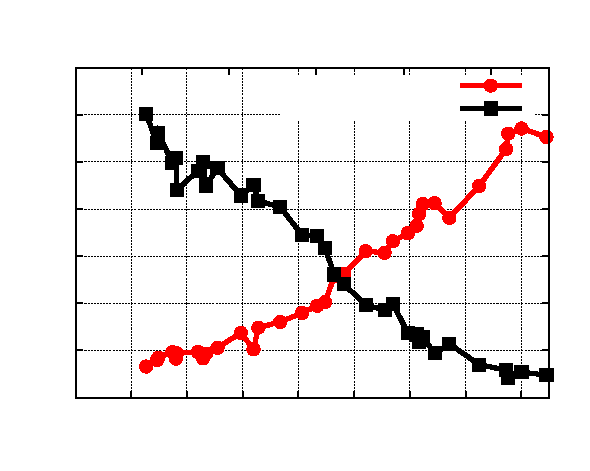
\includegraphics{SSLContrastVariationChiSquared400SSL}}%
    \gplfronttext
  \end{picture}%
\endgroup

		\caption{Variation of the 274.1 nm SSL bilayer scattering feature for increasing solvent osmolalities: normalized difference of the scattering curves at a certain sucrose concentration and in buffer. There are no sharp transitions, thus the osmotic effect is continuously modfying the bilayer structure.}
		\label{fig:SSLContrastVariationChiSquared400SSL}
\end{figure}

Besides, the changes of the phospholipid bilayer form factor are smooth upon increasing the osmotic pressure as shown in figure \ref{fig:SSLContrastVariationChiSquared400SSL}, where the bilayer feature scattering for increasing sucrose concentration is compared to the scattering curve of the SSL in buffer. This validates the observation from figure \ref{fig:SSLIsopointIntensity} and confirms that the increasing solvent osmotilality affects continuously the structure of the liposomes and not as abruptly as in the case of Caelyx.

Contrarily, the phospholipid bilayer of the plain liposomes remains invariable upon increasing the solvent osmolality until 1285 mOsm kg$^{-1}$, as displayed in figure \ref{fig:SSLContrastCurvesBilayer100Plain}. This suggests that the MLV structure of the non-PEGylated vesicles increase their resilience and the multiple phospholipid bilayers strengthen the elastic modulus of the liposome membrane.

The fact that the incorporation of PEG moieties influences already the preparation and formation of the liposomes prevents a proper comparison of the osmotic effects between SSLs and plain liposomes. In fact, the existence of MLVs for non-PEGylated liposomes acts as a limiting factor for the osmotic activity. This contrasts with the osmotic effects observed in SSLs already at low sucrose concentrations which shrinks the PEGylated liposomes into oblated ellipsoids. 

Although the chemical effect of sucrose on the SSL membrane can be discussed, previous studies in this subject \cite{kiselev_does_2003, kiselev_sucrose_2001, kiselev_sucrose_2001-1}, the large size of the sucrose molecule and similar results with other experiments performed with salt \cite{varga_osmotic_2014} validate this approach. The study of the osmotic activity of liposomes can be perfomed successfully using aqueous sucrose and shows very distinguishable effects for ULV (PEGylated liposomes) and MLV (plain liposomes).

%\begin{figure}
%	\centering
%		\subfloat[Scattering curves]{\resizebox{0.44\linewidth}{!}{% GNUPLOT: LaTeX picture with Postscript
\begingroup
  \makeatletter
  \providecommand\color[2][]{%
    \GenericError{(gnuplot) \space\space\space\@spaces}{%
      Package color not loaded in conjunction with
      terminal option `colourtext'%
    }{See the gnuplot documentation for explanation.%
    }{Either use 'blacktext' in gnuplot or load the package
      color.sty in LaTeX.}%
    \renewcommand\color[2][]{}%
  }%
  \providecommand\includegraphics[2][]{%
    \GenericError{(gnuplot) \space\space\space\@spaces}{%
      Package graphicx or graphics not loaded%
    }{See the gnuplot documentation for explanation.%
    }{The gnuplot epslatex terminal needs graphicx.sty or graphics.sty.}%
    \renewcommand\includegraphics[2][]{}%
  }%
  \providecommand\rotatebox[2]{#2}%
  \@ifundefined{ifGPcolor}{%
    \newif\ifGPcolor
    \GPcolortrue
  }{}%
  \@ifundefined{ifGPblacktext}{%
    \newif\ifGPblacktext
    \GPblacktextfalse
  }{}%
  % define a \g@addto@macro without @ in the name:
  \let\gplgaddtomacro\g@addto@macro
  % define empty templates for all commands taking text:
  \gdef\gplbacktext{}%
  \gdef\gplfronttext{}%
  \makeatother
  \ifGPblacktext
    % no textcolor at all
    \def\colorrgb#1{}%
    \def\colorgray#1{}%
  \else
    % gray or color?
    \ifGPcolor
      \def\colorrgb#1{\color[rgb]{#1}}%
      \def\colorgray#1{\color[gray]{#1}}%
      \expandafter\def\csname LTw\endcsname{\color{white}}%
      \expandafter\def\csname LTb\endcsname{\color{black}}%
      \expandafter\def\csname LTa\endcsname{\color{black}}%
      \expandafter\def\csname LT0\endcsname{\color[rgb]{1,0,0}}%
      \expandafter\def\csname LT1\endcsname{\color[rgb]{0,1,0}}%
      \expandafter\def\csname LT2\endcsname{\color[rgb]{0,0,1}}%
      \expandafter\def\csname LT3\endcsname{\color[rgb]{1,0,1}}%
      \expandafter\def\csname LT4\endcsname{\color[rgb]{0,1,1}}%
      \expandafter\def\csname LT5\endcsname{\color[rgb]{1,1,0}}%
      \expandafter\def\csname LT6\endcsname{\color[rgb]{0,0,0}}%
      \expandafter\def\csname LT7\endcsname{\color[rgb]{1,0.3,0}}%
      \expandafter\def\csname LT8\endcsname{\color[rgb]{0.5,0.5,0.5}}%
    \else
      % gray
      \def\colorrgb#1{\color{black}}%
      \def\colorgray#1{\color[gray]{#1}}%
      \expandafter\def\csname LTw\endcsname{\color{white}}%
      \expandafter\def\csname LTb\endcsname{\color{black}}%
      \expandafter\def\csname LTa\endcsname{\color{black}}%
      \expandafter\def\csname LT0\endcsname{\color{black}}%
      \expandafter\def\csname LT1\endcsname{\color{black}}%
      \expandafter\def\csname LT2\endcsname{\color{black}}%
      \expandafter\def\csname LT3\endcsname{\color{black}}%
      \expandafter\def\csname LT4\endcsname{\color{black}}%
      \expandafter\def\csname LT5\endcsname{\color{black}}%
      \expandafter\def\csname LT6\endcsname{\color{black}}%
      \expandafter\def\csname LT7\endcsname{\color{black}}%
      \expandafter\def\csname LT8\endcsname{\color{black}}%
    \fi
  \fi
    \setlength{\unitlength}{0.0500bp}%
    \ifx\gptboxheight\undefined%
      \newlength{\gptboxheight}%
      \newlength{\gptboxwidth}%
      \newsavebox{\gptboxtext}%
    \fi%
    \setlength{\fboxrule}{0.5pt}%
    \setlength{\fboxsep}{1pt}%
\begin{picture}(5668.00,4534.00)%
    \gplgaddtomacro\gplbacktext{%
      \csname LTb\endcsname%
      \put(880,1002){\makebox(0,0)[r]{\strut{}$1$}}%
      \csname LTb\endcsname%
      \put(880,1992){\makebox(0,0)[r]{\strut{}$10$}}%
      \csname LTb\endcsname%
      \put(880,2981){\makebox(0,0)[r]{\strut{}$100$}}%
      \csname LTb\endcsname%
      \put(880,3971){\makebox(0,0)[r]{\strut{}$1000$}}%
      \csname LTb\endcsname%
      \put(1613,484){\makebox(0,0){\strut{}$0.05$}}%
      \csname LTb\endcsname%
      \put(2429,484){\makebox(0,0){\strut{}$0.1$}}%
      \csname LTb\endcsname%
      \put(3244,484){\makebox(0,0){\strut{}$0.2$}}%
      \csname LTb\endcsname%
      \put(4322,484){\makebox(0,0){\strut{}$0.5$}}%
      \csname LTb\endcsname%
      \put(5138,484){\makebox(0,0){\strut{}$1$}}%
    }%
    \gplgaddtomacro\gplfronttext{%
      \csname LTb\endcsname%
      \put(176,2486){\rotatebox{-270}{\makebox(0,0){\strut{}Scattering Intensity / a.u.}}}%
      \put(3273,154){\makebox(0,0){\strut{}$q$ / nm$^{-1}$}}%
      \csname LTb\endcsname%
      \put(4284,4096){\makebox(0,0)[r]{\strut{}In buffer}}%
      \csname LTb\endcsname%
      \put(4284,3876){\makebox(0,0)[r]{\strut{}Max. osmolality}}%
    }%
    \gplbacktext
    \put(0,0){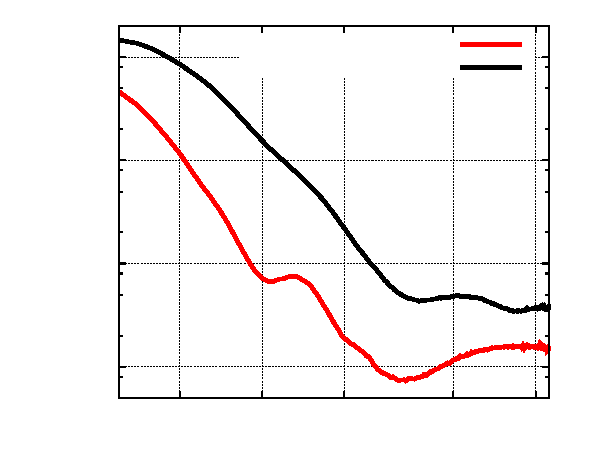
\includegraphics{SSLCurveFeatureComparison}}%
    \gplfronttext
  \end{picture}%
\endgroup
}\label{fig:SSLCurveFeatureComparison}}
%		\subfloat[Bilayer deformation]{\resizebox{0.44\linewidth}{!}{% GNUPLOT: LaTeX picture with Postscript
\begingroup
  \makeatletter
  \providecommand\color[2][]{%
    \GenericError{(gnuplot) \space\space\space\@spaces}{%
      Package color not loaded in conjunction with
      terminal option `colourtext'%
    }{See the gnuplot documentation for explanation.%
    }{Either use 'blacktext' in gnuplot or load the package
      color.sty in LaTeX.}%
    \renewcommand\color[2][]{}%
  }%
  \providecommand\includegraphics[2][]{%
    \GenericError{(gnuplot) \space\space\space\@spaces}{%
      Package graphicx or graphics not loaded%
    }{See the gnuplot documentation for explanation.%
    }{The gnuplot epslatex terminal needs graphicx.sty or graphics.sty.}%
    \renewcommand\includegraphics[2][]{}%
  }%
  \providecommand\rotatebox[2]{#2}%
  \@ifundefined{ifGPcolor}{%
    \newif\ifGPcolor
    \GPcolortrue
  }{}%
  \@ifundefined{ifGPblacktext}{%
    \newif\ifGPblacktext
    \GPblacktextfalse
  }{}%
  % define a \g@addto@macro without @ in the name:
  \let\gplgaddtomacro\g@addto@macro
  % define empty templates for all commands taking text:
  \gdef\gplbacktext{}%
  \gdef\gplfronttext{}%
  \makeatother
  \ifGPblacktext
    % no textcolor at all
    \def\colorrgb#1{}%
    \def\colorgray#1{}%
  \else
    % gray or color?
    \ifGPcolor
      \def\colorrgb#1{\color[rgb]{#1}}%
      \def\colorgray#1{\color[gray]{#1}}%
      \expandafter\def\csname LTw\endcsname{\color{white}}%
      \expandafter\def\csname LTb\endcsname{\color{black}}%
      \expandafter\def\csname LTa\endcsname{\color{black}}%
      \expandafter\def\csname LT0\endcsname{\color[rgb]{1,0,0}}%
      \expandafter\def\csname LT1\endcsname{\color[rgb]{0,1,0}}%
      \expandafter\def\csname LT2\endcsname{\color[rgb]{0,0,1}}%
      \expandafter\def\csname LT3\endcsname{\color[rgb]{1,0,1}}%
      \expandafter\def\csname LT4\endcsname{\color[rgb]{0,1,1}}%
      \expandafter\def\csname LT5\endcsname{\color[rgb]{1,1,0}}%
      \expandafter\def\csname LT6\endcsname{\color[rgb]{0,0,0}}%
      \expandafter\def\csname LT7\endcsname{\color[rgb]{1,0.3,0}}%
      \expandafter\def\csname LT8\endcsname{\color[rgb]{0.5,0.5,0.5}}%
    \else
      % gray
      \def\colorrgb#1{\color{black}}%
      \def\colorgray#1{\color[gray]{#1}}%
      \expandafter\def\csname LTw\endcsname{\color{white}}%
      \expandafter\def\csname LTb\endcsname{\color{black}}%
      \expandafter\def\csname LTa\endcsname{\color{black}}%
      \expandafter\def\csname LT0\endcsname{\color{black}}%
      \expandafter\def\csname LT1\endcsname{\color{black}}%
      \expandafter\def\csname LT2\endcsname{\color{black}}%
      \expandafter\def\csname LT3\endcsname{\color{black}}%
      \expandafter\def\csname LT4\endcsname{\color{black}}%
      \expandafter\def\csname LT5\endcsname{\color{black}}%
      \expandafter\def\csname LT6\endcsname{\color{black}}%
      \expandafter\def\csname LT7\endcsname{\color{black}}%
      \expandafter\def\csname LT8\endcsname{\color{black}}%
    \fi
  \fi
  \setlength{\unitlength}{0.0500bp}%
  \begin{picture}(5668.00,4534.00)%
    \gplgaddtomacro\gplbacktext{%
      \csname LTb\endcsname%
      \put(880,704){\makebox(0,0)[r]{\strut{} 0}}%
      \csname LTb\endcsname%
      \put(880,1298){\makebox(0,0)[r]{\strut{} 5}}%
      \csname LTb\endcsname%
      \put(880,1892){\makebox(0,0)[r]{\strut{} 10}}%
      \csname LTb\endcsname%
      \put(880,2487){\makebox(0,0)[r]{\strut{} 15}}%
      \csname LTb\endcsname%
      \put(880,3081){\makebox(0,0)[r]{\strut{} 20}}%
      \csname LTb\endcsname%
      \put(880,3675){\makebox(0,0)[r]{\strut{} 25}}%
      \csname LTb\endcsname%
      \put(880,4269){\makebox(0,0)[r]{\strut{} 30}}%
      \csname LTb\endcsname%
      \put(1012,484){\makebox(0,0){\strut{} 0}}%
      \csname LTb\endcsname%
      \put(1864,484){\makebox(0,0){\strut{} 5}}%
      \csname LTb\endcsname%
      \put(2716,484){\makebox(0,0){\strut{} 10}}%
      \csname LTb\endcsname%
      \put(3567,484){\makebox(0,0){\strut{} 15}}%
      \csname LTb\endcsname%
      \put(4419,484){\makebox(0,0){\strut{} 20}}%
      \csname LTb\endcsname%
      \put(5271,484){\makebox(0,0){\strut{} 25}}%
      \put(176,2486){\rotatebox{-270}{\makebox(0,0){\strut{}Normalized $\chi^2$}}}%
      \put(3273,154){\makebox(0,0){\strut{}Sucrose Mass Fraction / $\%$}}%
      \colorrgb{0.00,0.00,1.00}%
      \put(3567,2273){\makebox(0,0){\strut{}Bilayer}}%
      \put(3567,2053){\makebox(0,0){\strut{}Deformation}}%
    }%
    \gplgaddtomacro\gplfronttext{%
      \csname LTb\endcsname%
      \put(4284,4096){\makebox(0,0)[r]{\strut{}Diff. to SSL in buffer}}%
      \csname LTb\endcsname%
      \put(4284,3876){\makebox(0,0)[r]{\strut{}Diff. to SSL in max. osmolality}}%
    }%
    \gplbacktext
    \put(0,0){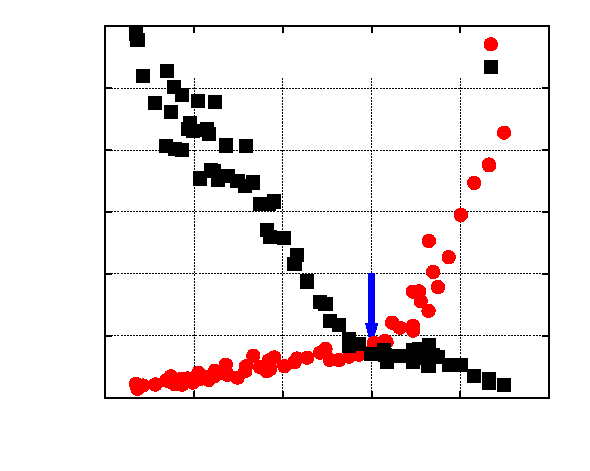
\includegraphics{SSLBilayerDeformationChi2}}%
    \gplfronttext
  \end{picture}%
\endgroup
}\label{fig:SSLBilayerDeformationChi2}}
%		\caption{Scattering curve of SSL 50 nm (Oct 2015) in aqueous buffer and at maximum concentration. The phospholipid bilayer feature appears at $q>0.3$ nm$^{-1}$ and changes drastically from one curve to the other. At the right, the bilayer deformation is observed for increasing sucrose mass fraction e.g. solvent osmolality.}
%\end{figure}


%\begin{figure}
%	\centering
%		\subfloat[Poisson Law]{\resizebox{0.44\linewidth}{!}{% GNUPLOT: LaTeX picture with Postscript
\begingroup
  \makeatletter
  \providecommand\color[2][]{%
    \GenericError{(gnuplot) \space\space\space\@spaces}{%
      Package color not loaded in conjunction with
      terminal option `colourtext'%
    }{See the gnuplot documentation for explanation.%
    }{Either use 'blacktext' in gnuplot or load the package
      color.sty in LaTeX.}%
    \renewcommand\color[2][]{}%
  }%
  \providecommand\includegraphics[2][]{%
    \GenericError{(gnuplot) \space\space\space\@spaces}{%
      Package graphicx or graphics not loaded%
    }{See the gnuplot documentation for explanation.%
    }{The gnuplot epslatex terminal needs graphicx.sty or graphics.sty.}%
    \renewcommand\includegraphics[2][]{}%
  }%
  \providecommand\rotatebox[2]{#2}%
  \@ifundefined{ifGPcolor}{%
    \newif\ifGPcolor
    \GPcolortrue
  }{}%
  \@ifundefined{ifGPblacktext}{%
    \newif\ifGPblacktext
    \GPblacktextfalse
  }{}%
  % define a \g@addto@macro without @ in the name:
  \let\gplgaddtomacro\g@addto@macro
  % define empty templates for all commands taking text:
  \gdef\gplbacktext{}%
  \gdef\gplfronttext{}%
  \makeatother
  \ifGPblacktext
    % no textcolor at all
    \def\colorrgb#1{}%
    \def\colorgray#1{}%
  \else
    % gray or color?
    \ifGPcolor
      \def\colorrgb#1{\color[rgb]{#1}}%
      \def\colorgray#1{\color[gray]{#1}}%
      \expandafter\def\csname LTw\endcsname{\color{white}}%
      \expandafter\def\csname LTb\endcsname{\color{black}}%
      \expandafter\def\csname LTa\endcsname{\color{black}}%
      \expandafter\def\csname LT0\endcsname{\color[rgb]{1,0,0}}%
      \expandafter\def\csname LT1\endcsname{\color[rgb]{0,1,0}}%
      \expandafter\def\csname LT2\endcsname{\color[rgb]{0,0,1}}%
      \expandafter\def\csname LT3\endcsname{\color[rgb]{1,0,1}}%
      \expandafter\def\csname LT4\endcsname{\color[rgb]{0,1,1}}%
      \expandafter\def\csname LT5\endcsname{\color[rgb]{1,1,0}}%
      \expandafter\def\csname LT6\endcsname{\color[rgb]{0,0,0}}%
      \expandafter\def\csname LT7\endcsname{\color[rgb]{1,0.3,0}}%
      \expandafter\def\csname LT8\endcsname{\color[rgb]{0.5,0.5,0.5}}%
    \else
      % gray
      \def\colorrgb#1{\color{black}}%
      \def\colorgray#1{\color[gray]{#1}}%
      \expandafter\def\csname LTw\endcsname{\color{white}}%
      \expandafter\def\csname LTb\endcsname{\color{black}}%
      \expandafter\def\csname LTa\endcsname{\color{black}}%
      \expandafter\def\csname LT0\endcsname{\color{black}}%
      \expandafter\def\csname LT1\endcsname{\color{black}}%
      \expandafter\def\csname LT2\endcsname{\color{black}}%
      \expandafter\def\csname LT3\endcsname{\color{black}}%
      \expandafter\def\csname LT4\endcsname{\color{black}}%
      \expandafter\def\csname LT5\endcsname{\color{black}}%
      \expandafter\def\csname LT6\endcsname{\color{black}}%
      \expandafter\def\csname LT7\endcsname{\color{black}}%
      \expandafter\def\csname LT8\endcsname{\color{black}}%
    \fi
  \fi
    \setlength{\unitlength}{0.0500bp}%
    \ifx\gptboxheight\undefined%
      \newlength{\gptboxheight}%
      \newlength{\gptboxwidth}%
      \newsavebox{\gptboxtext}%
    \fi%
    \setlength{\fboxrule}{0.5pt}%
    \setlength{\fboxsep}{1pt}%
\begin{picture}(5668.00,4534.00)%
    \gplgaddtomacro\gplbacktext{%
      \csname LTb\endcsname%
      \put(880,704){\makebox(0,0)[r]{\strut{}$180$}}%
      \csname LTb\endcsname%
      \put(880,1150){\makebox(0,0)[r]{\strut{}$190$}}%
      \csname LTb\endcsname%
      \put(880,1595){\makebox(0,0)[r]{\strut{}$200$}}%
      \csname LTb\endcsname%
      \put(880,2041){\makebox(0,0)[r]{\strut{}$210$}}%
      \csname LTb\endcsname%
      \put(880,2487){\makebox(0,0)[r]{\strut{}$220$}}%
      \csname LTb\endcsname%
      \put(880,2932){\makebox(0,0)[r]{\strut{}$230$}}%
      \csname LTb\endcsname%
      \put(880,3378){\makebox(0,0)[r]{\strut{}$240$}}%
      \csname LTb\endcsname%
      \put(880,3823){\makebox(0,0)[r]{\strut{}$250$}}%
      \csname LTb\endcsname%
      \put(880,4269){\makebox(0,0)[r]{\strut{}$260$}}%
      \csname LTb\endcsname%
      \put(1012,484){\makebox(0,0){\strut{}$0.019$}}%
      \csname LTb\endcsname%
      \put(1722,484){\makebox(0,0){\strut{}$0.02$}}%
      \csname LTb\endcsname%
      \put(2432,484){\makebox(0,0){\strut{}$0.021$}}%
      \csname LTb\endcsname%
      \put(3142,484){\makebox(0,0){\strut{}$0.022$}}%
      \csname LTb\endcsname%
      \put(3851,484){\makebox(0,0){\strut{}$0.023$}}%
      \csname LTb\endcsname%
      \put(4561,484){\makebox(0,0){\strut{}$0.024$}}%
      \csname LTb\endcsname%
      \put(5271,484){\makebox(0,0){\strut{}$0.025$}}%
    }%
    \gplgaddtomacro\gplfronttext{%
      \csname LTb\endcsname%
      \put(176,2486){\rotatebox{-270}{\makebox(0,0){\strut{}Pressure difference / mOsm kg$^{-1}$}}}%
      \put(3273,154){\makebox(0,0){\strut{}1/Radius / nm$^{-1}$}}%
    }%
    \gplbacktext
    \put(0,0){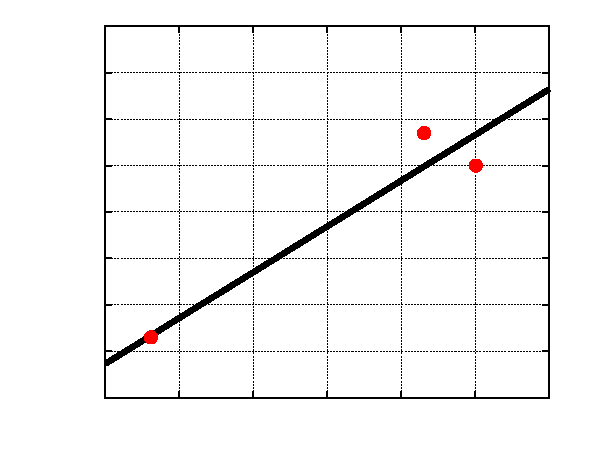
\includegraphics{SSLPoissonOsmoticShrinkage}}%
    \gplfronttext
  \end{picture}%
\endgroup
}\label{fig:SSLPoissonOsmoticShrinkage}}
%		\subfloat[Bilayer deformation and osmotic shrinkage]{\resizebox{0.44\linewidth}{!}{% GNUPLOT: LaTeX picture with Postscript
\begingroup
  \makeatletter
  \providecommand\color[2][]{%
    \GenericError{(gnuplot) \space\space\space\@spaces}{%
      Package color not loaded in conjunction with
      terminal option `colourtext'%
    }{See the gnuplot documentation for explanation.%
    }{Either use 'blacktext' in gnuplot or load the package
      color.sty in LaTeX.}%
    \renewcommand\color[2][]{}%
  }%
  \providecommand\includegraphics[2][]{%
    \GenericError{(gnuplot) \space\space\space\@spaces}{%
      Package graphicx or graphics not loaded%
    }{See the gnuplot documentation for explanation.%
    }{The gnuplot epslatex terminal needs graphicx.sty or graphics.sty.}%
    \renewcommand\includegraphics[2][]{}%
  }%
  \providecommand\rotatebox[2]{#2}%
  \@ifundefined{ifGPcolor}{%
    \newif\ifGPcolor
    \GPcolortrue
  }{}%
  \@ifundefined{ifGPblacktext}{%
    \newif\ifGPblacktext
    \GPblacktextfalse
  }{}%
  % define a \g@addto@macro without @ in the name:
  \let\gplgaddtomacro\g@addto@macro
  % define empty templates for all commands taking text:
  \gdef\gplbacktext{}%
  \gdef\gplfronttext{}%
  \makeatother
  \ifGPblacktext
    % no textcolor at all
    \def\colorrgb#1{}%
    \def\colorgray#1{}%
  \else
    % gray or color?
    \ifGPcolor
      \def\colorrgb#1{\color[rgb]{#1}}%
      \def\colorgray#1{\color[gray]{#1}}%
      \expandafter\def\csname LTw\endcsname{\color{white}}%
      \expandafter\def\csname LTb\endcsname{\color{black}}%
      \expandafter\def\csname LTa\endcsname{\color{black}}%
      \expandafter\def\csname LT0\endcsname{\color[rgb]{1,0,0}}%
      \expandafter\def\csname LT1\endcsname{\color[rgb]{0,1,0}}%
      \expandafter\def\csname LT2\endcsname{\color[rgb]{0,0,1}}%
      \expandafter\def\csname LT3\endcsname{\color[rgb]{1,0,1}}%
      \expandafter\def\csname LT4\endcsname{\color[rgb]{0,1,1}}%
      \expandafter\def\csname LT5\endcsname{\color[rgb]{1,1,0}}%
      \expandafter\def\csname LT6\endcsname{\color[rgb]{0,0,0}}%
      \expandafter\def\csname LT7\endcsname{\color[rgb]{1,0.3,0}}%
      \expandafter\def\csname LT8\endcsname{\color[rgb]{0.5,0.5,0.5}}%
    \else
      % gray
      \def\colorrgb#1{\color{black}}%
      \def\colorgray#1{\color[gray]{#1}}%
      \expandafter\def\csname LTw\endcsname{\color{white}}%
      \expandafter\def\csname LTb\endcsname{\color{black}}%
      \expandafter\def\csname LTa\endcsname{\color{black}}%
      \expandafter\def\csname LT0\endcsname{\color{black}}%
      \expandafter\def\csname LT1\endcsname{\color{black}}%
      \expandafter\def\csname LT2\endcsname{\color{black}}%
      \expandafter\def\csname LT3\endcsname{\color{black}}%
      \expandafter\def\csname LT4\endcsname{\color{black}}%
      \expandafter\def\csname LT5\endcsname{\color{black}}%
      \expandafter\def\csname LT6\endcsname{\color{black}}%
      \expandafter\def\csname LT7\endcsname{\color{black}}%
      \expandafter\def\csname LT8\endcsname{\color{black}}%
    \fi
  \fi
  \setlength{\unitlength}{0.0500bp}%
  \begin{picture}(5668.00,4534.00)%
    \gplgaddtomacro\gplbacktext{%
      \csname LTb\endcsname%
      \put(1012,1014){\makebox(0,0)[r]{\strut{} 200}}%
      \csname LTb\endcsname%
      \put(1012,1402){\makebox(0,0)[r]{\strut{} 250}}%
      \csname LTb\endcsname%
      \put(1012,1789){\makebox(0,0)[r]{\strut{} 300}}%
      \csname LTb\endcsname%
      \put(1012,2177){\makebox(0,0)[r]{\strut{} 350}}%
      \csname LTb\endcsname%
      \put(1012,2564){\makebox(0,0)[r]{\strut{} 400}}%
      \csname LTb\endcsname%
      \put(1012,2952){\makebox(0,0)[r]{\strut{} 450}}%
      \csname LTb\endcsname%
      \put(1012,3339){\makebox(0,0)[r]{\strut{} 500}}%
      \csname LTb\endcsname%
      \put(1012,3727){\makebox(0,0)[r]{\strut{} 550}}%
      \csname LTb\endcsname%
      \put(1012,4114){\makebox(0,0)[r]{\strut{} 600}}%
      \csname LTb\endcsname%
      \put(1144,484){\makebox(0,0){\strut{} 0.014}}%
      \csname LTb\endcsname%
      \put(1894,484){\makebox(0,0){\strut{} 0.016}}%
      \csname LTb\endcsname%
      \put(2645,484){\makebox(0,0){\strut{} 0.018}}%
      \csname LTb\endcsname%
      \put(3395,484){\makebox(0,0){\strut{} 0.02}}%
      \csname LTb\endcsname%
      \put(4145,484){\makebox(0,0){\strut{} 0.022}}%
      \csname LTb\endcsname%
      \put(4896,484){\makebox(0,0){\strut{} 0.024}}%
      \put(176,2486){\rotatebox{-270}{\makebox(0,0){\strut{}Pressure difference / mOsm kg$^{-1}$}}}%
      \put(3339,154){\makebox(0,0){\strut{}1/Radius / nm$^{-1}$}}%
      \colorrgb{0.00,0.00,0.00}%
      \put(2270,1324){\makebox(0,0)[l]{\strut{}Osmotic Shrinkage}}%
      \colorrgb{0.80,0.31,0.31}%
      \put(3770,3107){\makebox(0,0)[l]{\strut{}HSPC+PEG}}%
      \colorrgb{0.43,0.42,0.82}%
      \put(1894,3727){\makebox(0,0)[l]{\strut{}HSPC}}%
      \colorrgb{0.00,0.00,0.00}%
      \put(3770,2254){\makebox(0,0)[l]{\strut{}Caelyx}}%
    }%
    \gplgaddtomacro\gplfronttext{%
    }%
    \gplbacktext
    \put(0,0){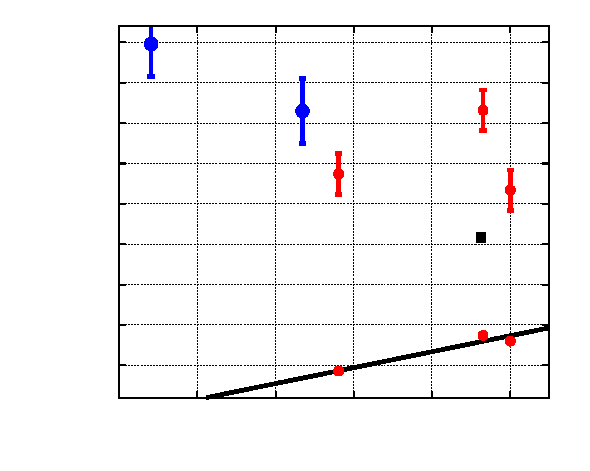
\includegraphics{SSLPoissonComplete}}%
    \gplfronttext
  \end{picture}%
\endgroup
}\label{fig:SSLPoissonComplete}}
%		\caption{Summary of the different osmotic pressures needed for the deformation of the liposamal structure. The radius was determined by DLS.}
%\end{figure}


\section{Sizing of blood plasma componenents}
\label{sec:lipoprotein_continuous}

From a nanoscience point of view, human blood can be seen as a suspension of particles with different physiological roles. Serum lipoproteins are the colloidal particles involved in the transport and metabolism of insoluble lipids and are among the most studied biological particles. The interest in their activity is understandable due to their direct relationship with very extended diseases in the Western world population, such as morbidity or atherogenesis, e.g. obturation of the arterial walls. For example, the dysregulation of cholesterol in plasma, primarly carried within lipoproteins, is responsible of atherosclerosis \cite{munro_pathogenesis_1988}. Besides, they are a convenient model for lipid-protein interactions \cite{assmann_lipid-protein_1974} due to their lipid core and the hydrated proteins isometrically situated on its surface.

Lipoproteins are normally classified by the density range within they are isolated from blood plasma by ultracentrifugation \cite{havel_distribution_1955}, showing different chemical composition, size and pathological condition for each class \cite{german_lipoproteins:_2006}. Indeed, the size of lipoproteins is critically connected with disease risk \cite{gardner_cd_association_1996} and Low-density Lipoproteins (LDL) are suggested to be more or less atherogenic depending on their size \cite{dreon_low-density_1994}. The effect of diabetes on the lipoprotein size is also of great interest, specially the sex-dependency of High-density Lipoproteins (HDL) size \cite{colhoun_lipoprotein_2002}.

Therefore, precise sizing techniques are a crucial tool to understand the physiological processes of lipoproteins \cite{german_lipoproteins:_2006}. The naturally narrow size distributions of LDL and HDL suggest small-angle scattering as a well-suited method and their heterogenous morphology advises the use of a contrast variation approach. For instance, the first characterization attempts date back to the late 1970s with neutron scattering \cite{stuhrmann_neutron_1975}, using salt \cite{tardieu_structure_1976} and sucrose \cite{muller_structure_1978} as SAXS contrast agents or modifying the sample temperature \cite{laggner_molecular_1977,luzzati_structure_1979}. 

\begin{figure}
	\centering
		\subfloat[HDL]{\resizebox{0.44\linewidth}{!}{% GNUPLOT: LaTeX picture with Postscript
\begingroup
  \makeatletter
  \providecommand\color[2][]{%
    \GenericError{(gnuplot) \space\space\space\@spaces}{%
      Package color not loaded in conjunction with
      terminal option `colourtext'%
    }{See the gnuplot documentation for explanation.%
    }{Either use 'blacktext' in gnuplot or load the package
      color.sty in LaTeX.}%
    \renewcommand\color[2][]{}%
  }%
  \providecommand\includegraphics[2][]{%
    \GenericError{(gnuplot) \space\space\space\@spaces}{%
      Package graphicx or graphics not loaded%
    }{See the gnuplot documentation for explanation.%
    }{The gnuplot epslatex terminal needs graphicx.sty or graphics.sty.}%
    \renewcommand\includegraphics[2][]{}%
  }%
  \providecommand\rotatebox[2]{#2}%
  \@ifundefined{ifGPcolor}{%
    \newif\ifGPcolor
    \GPcolortrue
  }{}%
  \@ifundefined{ifGPblacktext}{%
    \newif\ifGPblacktext
    \GPblacktextfalse
  }{}%
  % define a \g@addto@macro without @ in the name:
  \let\gplgaddtomacro\g@addto@macro
  % define empty templates for all commands taking text:
  \gdef\gplbacktext{}%
  \gdef\gplfronttext{}%
  \makeatother
  \ifGPblacktext
    % no textcolor at all
    \def\colorrgb#1{}%
    \def\colorgray#1{}%
  \else
    % gray or color?
    \ifGPcolor
      \def\colorrgb#1{\color[rgb]{#1}}%
      \def\colorgray#1{\color[gray]{#1}}%
      \expandafter\def\csname LTw\endcsname{\color{white}}%
      \expandafter\def\csname LTb\endcsname{\color{black}}%
      \expandafter\def\csname LTa\endcsname{\color{black}}%
      \expandafter\def\csname LT0\endcsname{\color[rgb]{1,0,0}}%
      \expandafter\def\csname LT1\endcsname{\color[rgb]{0,1,0}}%
      \expandafter\def\csname LT2\endcsname{\color[rgb]{0,0,1}}%
      \expandafter\def\csname LT3\endcsname{\color[rgb]{1,0,1}}%
      \expandafter\def\csname LT4\endcsname{\color[rgb]{0,1,1}}%
      \expandafter\def\csname LT5\endcsname{\color[rgb]{1,1,0}}%
      \expandafter\def\csname LT6\endcsname{\color[rgb]{0,0,0}}%
      \expandafter\def\csname LT7\endcsname{\color[rgb]{1,0.3,0}}%
      \expandafter\def\csname LT8\endcsname{\color[rgb]{0.5,0.5,0.5}}%
    \else
      % gray
      \def\colorrgb#1{\color{black}}%
      \def\colorgray#1{\color[gray]{#1}}%
      \expandafter\def\csname LTw\endcsname{\color{white}}%
      \expandafter\def\csname LTb\endcsname{\color{black}}%
      \expandafter\def\csname LTa\endcsname{\color{black}}%
      \expandafter\def\csname LT0\endcsname{\color{black}}%
      \expandafter\def\csname LT1\endcsname{\color{black}}%
      \expandafter\def\csname LT2\endcsname{\color{black}}%
      \expandafter\def\csname LT3\endcsname{\color{black}}%
      \expandafter\def\csname LT4\endcsname{\color{black}}%
      \expandafter\def\csname LT5\endcsname{\color{black}}%
      \expandafter\def\csname LT6\endcsname{\color{black}}%
      \expandafter\def\csname LT7\endcsname{\color{black}}%
      \expandafter\def\csname LT8\endcsname{\color{black}}%
    \fi
  \fi
  \setlength{\unitlength}{0.0500bp}%
  \begin{picture}(5668.00,4534.00)%
    \gplgaddtomacro\gplbacktext{%
      \csname LTb\endcsname%
      \put(814,704){\makebox(0,0)[r]{\strut{} 0.1}}%
      \csname LTb\endcsname%
      \put(814,2025){\makebox(0,0)[r]{\strut{} 1}}%
      \csname LTb\endcsname%
      \put(814,3346){\makebox(0,0)[r]{\strut{} 10}}%
      \csname LTb\endcsname%
      \put(1532,484){\makebox(0,0){\strut{} 0.2}}%
      \csname LTb\endcsname%
      \put(2583,484){\makebox(0,0){\strut{} 0.5}}%
      \csname LTb\endcsname%
      \put(3378,484){\makebox(0,0){\strut{} 1}}%
      \csname LTb\endcsname%
      \put(4173,484){\makebox(0,0){\strut{} 2}}%
      \put(176,2266){\rotatebox{-270}{\makebox(0,0){\strut{}Scattering Intensity / a.u.}}}%
      \put(2687,154){\makebox(0,0){\strut{}$q$ / nm$^{-1}$}}%
    }%
    \gplgaddtomacro\gplfronttext{%
      \csname LTb\endcsname%
      \put(4822,1147){\makebox(0,0)[l]{\strut{}\smaller 340}}%
      \put(4822,1841){\makebox(0,0)[l]{\strut{}\smaller 350}}%
      \put(4822,2535){\makebox(0,0)[l]{\strut{}\smaller 360}}%
      \put(4822,3228){\makebox(0,0)[l]{\strut{}\smaller 370}}%
      \put(4822,3922){\makebox(0,0)[l]{\strut{}\smaller 380}}%
      \put(5351,2486){\rotatebox{-90}{\makebox(0,0){\strut{}\smaller Solvent Electron Density / nm$^{-3}$}}}%
    }%
    \gplbacktext
    \put(0,0){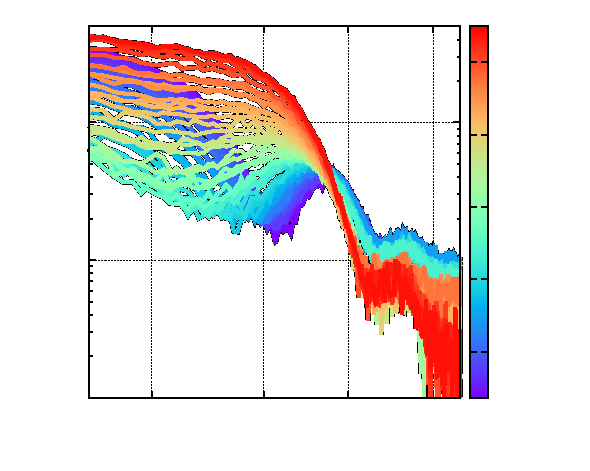
\includegraphics{HDLContinuousSAXS}}%
    \gplfronttext
  \end{picture}%
\endgroup
}\label{fig:HDLContinuousSAXS}}
		\subfloat[LDL]{\resizebox{0.44\linewidth}{!}{% GNUPLOT: LaTeX picture with Postscript
\begingroup
  \makeatletter
  \providecommand\color[2][]{%
    \GenericError{(gnuplot) \space\space\space\@spaces}{%
      Package color not loaded in conjunction with
      terminal option `colourtext'%
    }{See the gnuplot documentation for explanation.%
    }{Either use 'blacktext' in gnuplot or load the package
      color.sty in LaTeX.}%
    \renewcommand\color[2][]{}%
  }%
  \providecommand\includegraphics[2][]{%
    \GenericError{(gnuplot) \space\space\space\@spaces}{%
      Package graphicx or graphics not loaded%
    }{See the gnuplot documentation for explanation.%
    }{The gnuplot epslatex terminal needs graphicx.sty or graphics.sty.}%
    \renewcommand\includegraphics[2][]{}%
  }%
  \providecommand\rotatebox[2]{#2}%
  \@ifundefined{ifGPcolor}{%
    \newif\ifGPcolor
    \GPcolortrue
  }{}%
  \@ifundefined{ifGPblacktext}{%
    \newif\ifGPblacktext
    \GPblacktextfalse
  }{}%
  % define a \g@addto@macro without @ in the name:
  \let\gplgaddtomacro\g@addto@macro
  % define empty templates for all commands taking text:
  \gdef\gplbacktext{}%
  \gdef\gplfronttext{}%
  \makeatother
  \ifGPblacktext
    % no textcolor at all
    \def\colorrgb#1{}%
    \def\colorgray#1{}%
  \else
    % gray or color?
    \ifGPcolor
      \def\colorrgb#1{\color[rgb]{#1}}%
      \def\colorgray#1{\color[gray]{#1}}%
      \expandafter\def\csname LTw\endcsname{\color{white}}%
      \expandafter\def\csname LTb\endcsname{\color{black}}%
      \expandafter\def\csname LTa\endcsname{\color{black}}%
      \expandafter\def\csname LT0\endcsname{\color[rgb]{1,0,0}}%
      \expandafter\def\csname LT1\endcsname{\color[rgb]{0,1,0}}%
      \expandafter\def\csname LT2\endcsname{\color[rgb]{0,0,1}}%
      \expandafter\def\csname LT3\endcsname{\color[rgb]{1,0,1}}%
      \expandafter\def\csname LT4\endcsname{\color[rgb]{0,1,1}}%
      \expandafter\def\csname LT5\endcsname{\color[rgb]{1,1,0}}%
      \expandafter\def\csname LT6\endcsname{\color[rgb]{0,0,0}}%
      \expandafter\def\csname LT7\endcsname{\color[rgb]{1,0.3,0}}%
      \expandafter\def\csname LT8\endcsname{\color[rgb]{0.5,0.5,0.5}}%
    \else
      % gray
      \def\colorrgb#1{\color{black}}%
      \def\colorgray#1{\color[gray]{#1}}%
      \expandafter\def\csname LTw\endcsname{\color{white}}%
      \expandafter\def\csname LTb\endcsname{\color{black}}%
      \expandafter\def\csname LTa\endcsname{\color{black}}%
      \expandafter\def\csname LT0\endcsname{\color{black}}%
      \expandafter\def\csname LT1\endcsname{\color{black}}%
      \expandafter\def\csname LT2\endcsname{\color{black}}%
      \expandafter\def\csname LT3\endcsname{\color{black}}%
      \expandafter\def\csname LT4\endcsname{\color{black}}%
      \expandafter\def\csname LT5\endcsname{\color{black}}%
      \expandafter\def\csname LT6\endcsname{\color{black}}%
      \expandafter\def\csname LT7\endcsname{\color{black}}%
      \expandafter\def\csname LT8\endcsname{\color{black}}%
    \fi
  \fi
  \setlength{\unitlength}{0.0500bp}%
  \begin{picture}(5668.00,4534.00)%
    \gplgaddtomacro\gplbacktext{%
      \csname LTb\endcsname%
      \put(726,1062){\makebox(0,0)[r]{\strut{} 1}}%
      \csname LTb\endcsname%
      \put(726,2250){\makebox(0,0)[r]{\strut{} 10}}%
      \csname LTb\endcsname%
      \put(726,3438){\makebox(0,0)[r]{\strut{} 100}}%
      \csname LTb\endcsname%
      \put(1505,484){\makebox(0,0){\strut{} 0.2}}%
      \csname LTb\endcsname%
      \put(2665,484){\makebox(0,0){\strut{} 0.5}}%
      \csname LTb\endcsname%
      \put(3542,484){\makebox(0,0){\strut{} 1}}%
      \csname LTb\endcsname%
      \put(4420,484){\makebox(0,0){\strut{} 2}}%
      \put(220,2266){\rotatebox{-270}{\makebox(0,0){\strut{}Scattering Intensity / a.u.}}}%
      \put(2639,154){\makebox(0,0){\strut{}$q$ / nm$^{-1}$}}%
    }%
    \gplgaddtomacro\gplfronttext{%
      \csname LTb\endcsname%
      \put(4688,1147){\makebox(0,0)[l]{\strut{}340.0}}%
      \put(4688,1841){\makebox(0,0)[l]{\strut{}350.0}}%
      \put(4688,2535){\makebox(0,0)[l]{\strut{}360.0}}%
      \put(4688,3228){\makebox(0,0)[l]{\strut{}370.0}}%
      \put(4688,3922){\makebox(0,0)[l]{\strut{}380.0}}%
      \put(5414,2486){\rotatebox{-90}{\makebox(0,0){\strut{}\fsmedium Solvent Electron Density / nm$^{-3}$}}}%
    }%
    \gplbacktext
    \put(0,0){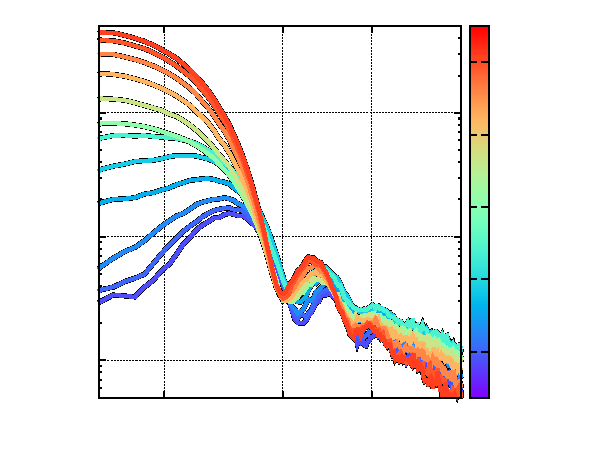
\includegraphics{LDLContinuousSAXS}}%
    \gplfronttext
  \end{picture}%
\endgroup
}\label{fig:LDLContinuousSAXS}}
		\caption{Scattering curves of HDL and LDL measured at different solvent densities by using an aqueous sucrose density gradient.}
\end{figure}

The complicated inner structure of the lipoproteins revealed in more recent studies \cite{baumstark_structure_1990,schnitzer_re-evaluation_1994} encourages the use of parameter-independent and model-free analysis of the scattering data. With this objective, LDL and HDL samples were measured with continuous contrast variation in SAXS using 40 $\%$ sucrose mass fraction to increase the solvent electron density until 384 nm$^{-3}$. The scattering curves obtained for HDL and LDL are presented in figures \ref{fig:HDLContinuousSAXS} and \ref{fig:LDLContinuousSAXS} respectively.

In the case of HDL in buffer, the first minimum appears at $q\approx0.5$ nm$^{-1}$ as already observed in figure \ref{fig:HDLCoreShellFit}. By increasing the solvent density, this minimum shifts to smaller $q$-values hinting the denser composition of the protein shell in comparison to the lighter lipid and cholesterol core. A lighter core morphology is also expected for LDL \cite{luzzati_structure_1979} and it agrees with the contrast effect observed in the scattering curves displayed in figure \ref{fig:LDLContinuousSAXS}.

\begin{figure}
	\centering
		\subfloat[Isoscattering point position]{\resizebox{0.44\linewidth}{!}{% GNUPLOT: LaTeX picture with Postscript
\begingroup
  \makeatletter
  \providecommand\color[2][]{%
    \GenericError{(gnuplot) \space\space\space\@spaces}{%
      Package color not loaded in conjunction with
      terminal option `colourtext'%
    }{See the gnuplot documentation for explanation.%
    }{Either use 'blacktext' in gnuplot or load the package
      color.sty in LaTeX.}%
    \renewcommand\color[2][]{}%
  }%
  \providecommand\includegraphics[2][]{%
    \GenericError{(gnuplot) \space\space\space\@spaces}{%
      Package graphicx or graphics not loaded%
    }{See the gnuplot documentation for explanation.%
    }{The gnuplot epslatex terminal needs graphicx.sty or graphics.sty.}%
    \renewcommand\includegraphics[2][]{}%
  }%
  \providecommand\rotatebox[2]{#2}%
  \@ifundefined{ifGPcolor}{%
    \newif\ifGPcolor
    \GPcolortrue
  }{}%
  \@ifundefined{ifGPblacktext}{%
    \newif\ifGPblacktext
    \GPblacktextfalse
  }{}%
  % define a \g@addto@macro without @ in the name:
  \let\gplgaddtomacro\g@addto@macro
  % define empty templates for all commands taking text:
  \gdef\gplbacktext{}%
  \gdef\gplfronttext{}%
  \makeatother
  \ifGPblacktext
    % no textcolor at all
    \def\colorrgb#1{}%
    \def\colorgray#1{}%
  \else
    % gray or color?
    \ifGPcolor
      \def\colorrgb#1{\color[rgb]{#1}}%
      \def\colorgray#1{\color[gray]{#1}}%
      \expandafter\def\csname LTw\endcsname{\color{white}}%
      \expandafter\def\csname LTb\endcsname{\color{black}}%
      \expandafter\def\csname LTa\endcsname{\color{black}}%
      \expandafter\def\csname LT0\endcsname{\color[rgb]{1,0,0}}%
      \expandafter\def\csname LT1\endcsname{\color[rgb]{0,1,0}}%
      \expandafter\def\csname LT2\endcsname{\color[rgb]{0,0,1}}%
      \expandafter\def\csname LT3\endcsname{\color[rgb]{1,0,1}}%
      \expandafter\def\csname LT4\endcsname{\color[rgb]{0,1,1}}%
      \expandafter\def\csname LT5\endcsname{\color[rgb]{1,1,0}}%
      \expandafter\def\csname LT6\endcsname{\color[rgb]{0,0,0}}%
      \expandafter\def\csname LT7\endcsname{\color[rgb]{1,0.3,0}}%
      \expandafter\def\csname LT8\endcsname{\color[rgb]{0.5,0.5,0.5}}%
    \else
      % gray
      \def\colorrgb#1{\color{black}}%
      \def\colorgray#1{\color[gray]{#1}}%
      \expandafter\def\csname LTw\endcsname{\color{white}}%
      \expandafter\def\csname LTb\endcsname{\color{black}}%
      \expandafter\def\csname LTa\endcsname{\color{black}}%
      \expandafter\def\csname LT0\endcsname{\color{black}}%
      \expandafter\def\csname LT1\endcsname{\color{black}}%
      \expandafter\def\csname LT2\endcsname{\color{black}}%
      \expandafter\def\csname LT3\endcsname{\color{black}}%
      \expandafter\def\csname LT4\endcsname{\color{black}}%
      \expandafter\def\csname LT5\endcsname{\color{black}}%
      \expandafter\def\csname LT6\endcsname{\color{black}}%
      \expandafter\def\csname LT7\endcsname{\color{black}}%
      \expandafter\def\csname LT8\endcsname{\color{black}}%
    \fi
  \fi
    \setlength{\unitlength}{0.0500bp}%
    \ifx\gptboxheight\undefined%
      \newlength{\gptboxheight}%
      \newlength{\gptboxwidth}%
      \newsavebox{\gptboxtext}%
    \fi%
    \setlength{\fboxrule}{0.5pt}%
    \setlength{\fboxsep}{1pt}%
\begin{picture}(5668.00,4534.00)%
    \gplgaddtomacro\gplbacktext{%
      \csname LTb\endcsname%
      \put(814,1351){\makebox(0,0)[r]{\strut{}$0.1$}}%
      \csname LTb\endcsname%
      \put(814,2230){\makebox(0,0)[r]{\strut{}$0.2$}}%
      \csname LTb\endcsname%
      \put(814,3391){\makebox(0,0)[r]{\strut{}$0.5$}}%
      \csname LTb\endcsname%
      \put(814,4269){\makebox(0,0)[r]{\strut{}$1$}}%
      \csname LTb\endcsname%
      \put(946,484){\makebox(0,0){\strut{}$0.3$}}%
      \csname LTb\endcsname%
      \put(2319,484){\makebox(0,0){\strut{}$0.5$}}%
      \csname LTb\endcsname%
      \put(4181,484){\makebox(0,0){\strut{}$1$}}%
      \csname LTb\endcsname%
      \put(5271,484){\makebox(0,0){\strut{}$1.5$}}%
    }%
    \gplgaddtomacro\gplfronttext{%
      \csname LTb\endcsname%
      \put(176,2486){\rotatebox{-270}{\makebox(0,0){\strut{}Rel. Std. Deviation}}}%
      \put(3108,154){\makebox(0,0){\strut{}$q$ / nm$^{-1}$}}%
      \csname LTb\endcsname%
      \put(4548,4041){\makebox(0,0)[r]{\strut{}\smaller HDL}}%
      \csname LTb\endcsname%
      \put(4548,3711){\makebox(0,0)[r]{\strut{}\smaller LDL}}%
    }%
    \gplbacktext
    \put(0,0){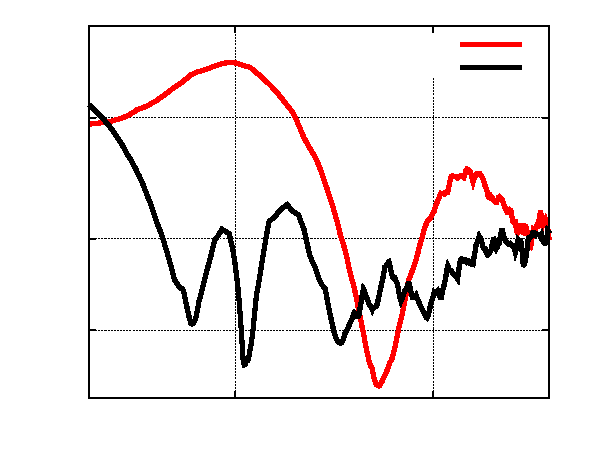
\includegraphics{LipoproteinIsopointComp}}%
    \gplfronttext
  \end{picture}%
\endgroup
}\label{fig:LipoproteinIsopointComp}}
		\subfloat[Average electron density]{\resizebox{0.44\linewidth}{!}{% GNUPLOT: LaTeX picture with Postscript
\begingroup
  \makeatletter
  \providecommand\color[2][]{%
    \GenericError{(gnuplot) \space\space\space\@spaces}{%
      Package color not loaded in conjunction with
      terminal option `colourtext'%
    }{See the gnuplot documentation for explanation.%
    }{Either use 'blacktext' in gnuplot or load the package
      color.sty in LaTeX.}%
    \renewcommand\color[2][]{}%
  }%
  \providecommand\includegraphics[2][]{%
    \GenericError{(gnuplot) \space\space\space\@spaces}{%
      Package graphicx or graphics not loaded%
    }{See the gnuplot documentation for explanation.%
    }{The gnuplot epslatex terminal needs graphicx.sty or graphics.sty.}%
    \renewcommand\includegraphics[2][]{}%
  }%
  \providecommand\rotatebox[2]{#2}%
  \@ifundefined{ifGPcolor}{%
    \newif\ifGPcolor
    \GPcolortrue
  }{}%
  \@ifundefined{ifGPblacktext}{%
    \newif\ifGPblacktext
    \GPblacktextfalse
  }{}%
  % define a \g@addto@macro without @ in the name:
  \let\gplgaddtomacro\g@addto@macro
  % define empty templates for all commands taking text:
  \gdef\gplbacktext{}%
  \gdef\gplfronttext{}%
  \makeatother
  \ifGPblacktext
    % no textcolor at all
    \def\colorrgb#1{}%
    \def\colorgray#1{}%
  \else
    % gray or color?
    \ifGPcolor
      \def\colorrgb#1{\color[rgb]{#1}}%
      \def\colorgray#1{\color[gray]{#1}}%
      \expandafter\def\csname LTw\endcsname{\color{white}}%
      \expandafter\def\csname LTb\endcsname{\color{black}}%
      \expandafter\def\csname LTa\endcsname{\color{black}}%
      \expandafter\def\csname LT0\endcsname{\color[rgb]{1,0,0}}%
      \expandafter\def\csname LT1\endcsname{\color[rgb]{0,1,0}}%
      \expandafter\def\csname LT2\endcsname{\color[rgb]{0,0,1}}%
      \expandafter\def\csname LT3\endcsname{\color[rgb]{1,0,1}}%
      \expandafter\def\csname LT4\endcsname{\color[rgb]{0,1,1}}%
      \expandafter\def\csname LT5\endcsname{\color[rgb]{1,1,0}}%
      \expandafter\def\csname LT6\endcsname{\color[rgb]{0,0,0}}%
      \expandafter\def\csname LT7\endcsname{\color[rgb]{1,0.3,0}}%
      \expandafter\def\csname LT8\endcsname{\color[rgb]{0.5,0.5,0.5}}%
    \else
      % gray
      \def\colorrgb#1{\color{black}}%
      \def\colorgray#1{\color[gray]{#1}}%
      \expandafter\def\csname LTw\endcsname{\color{white}}%
      \expandafter\def\csname LTb\endcsname{\color{black}}%
      \expandafter\def\csname LTa\endcsname{\color{black}}%
      \expandafter\def\csname LT0\endcsname{\color{black}}%
      \expandafter\def\csname LT1\endcsname{\color{black}}%
      \expandafter\def\csname LT2\endcsname{\color{black}}%
      \expandafter\def\csname LT3\endcsname{\color{black}}%
      \expandafter\def\csname LT4\endcsname{\color{black}}%
      \expandafter\def\csname LT5\endcsname{\color{black}}%
      \expandafter\def\csname LT6\endcsname{\color{black}}%
      \expandafter\def\csname LT7\endcsname{\color{black}}%
      \expandafter\def\csname LT8\endcsname{\color{black}}%
    \fi
  \fi
  \setlength{\unitlength}{0.0500bp}%
  \begin{picture}(5668.00,4534.00)%
    \gplgaddtomacro\gplbacktext{%
      \csname LTb\endcsname%
      \put(814,841){\makebox(0,0)[r]{\strut{} 0}}%
      \csname LTb\endcsname%
      \put(814,1527){\makebox(0,0)[r]{\strut{} 0.5}}%
      \csname LTb\endcsname%
      \put(814,2212){\makebox(0,0)[r]{\strut{} 1}}%
      \csname LTb\endcsname%
      \put(814,2898){\makebox(0,0)[r]{\strut{} 1.5}}%
      \csname LTb\endcsname%
      \put(814,3583){\makebox(0,0)[r]{\strut{} 2}}%
      \csname LTb\endcsname%
      \put(814,4269){\makebox(0,0)[r]{\strut{} 2.5}}%
      \csname LTb\endcsname%
      \put(1528,484){\makebox(0,0){\strut{} 340}}%
      \csname LTb\endcsname%
      \put(2360,484){\makebox(0,0){\strut{} 350}}%
      \csname LTb\endcsname%
      \put(3192,484){\makebox(0,0){\strut{} 360}}%
      \csname LTb\endcsname%
      \put(4023,484){\makebox(0,0){\strut{} 370}}%
      \csname LTb\endcsname%
      \put(4855,484){\makebox(0,0){\strut{} 380}}%
      \put(176,2486){\rotatebox{-270}{\makebox(0,0){\strut{}$I(0)$ / a.u.}}}%
      \put(3108,154){\makebox(0,0){\strut{}Solvent Electron Density / nm$^{-3}$}}%
    }%
    \gplgaddtomacro\gplfronttext{%
      \csname LTb\endcsname%
      \put(4098,4035){\makebox(0,0)[r]{\strut{}\smaller HDL}}%
      \csname LTb\endcsname%
      \put(4098,3705){\makebox(0,0)[r]{\strut{}\smaller LDL}}%
    }%
    \gplbacktext
    \put(0,0){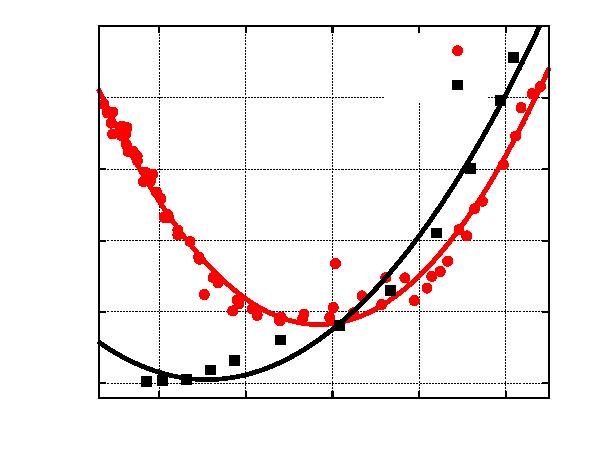
\includegraphics{LipoproteinsAverageDensity}}%
    \gplfronttext
  \end{picture}%
\endgroup
}\label{fig:LipoproteinsAverageDensity}}
		\caption{Comparison of the model free approaches for HDL (red) and LDL (black)}
\end{figure}

The appearance of so many minima indicates the narrow size distributions of both samples, providing the ideal conditions to use the isoscattering point $q^{\star}$ approach. The relative standard deviation as a function of $q$ calculated for both lipoproteins is shown in figure \ref{fig:LipoproteinIsopointComp}, where the minima correspond to the position of $q^{\star}_i$. The clear minimum for HDL is located at $q^{\star}=0.826$ nm$^{-1}$, correspondig to an impenetrable size for the solvent of 11 nm. The position of the first $q^{\star}$ in LDL is shifted to smaller $q$, $q^{\star}=0.42$ nm$^{-1}$, which translates into a solvent-excluded diameter of 21 nm.

Considering that the lipoproteins are quasi-spherical \cite{stuhrmann_neutron_1975}, these results can be compared to those extracted from literature. The different cholesterol tranport necessities reflect into a large variety of HDL subclasses with a size range between 7 and 13 nm \cite{german_lipoproteins:_2006}. For example, a size of 13 nm was observed for the HDL3 subfraction \cite{tardieu_structure_1976}, which deviates only 15 $\%$ from the result measured in our study. Difficulties to know the measured subclass of HDL hinders a more thorough comparison.

In the case of LDL, several studies provide diameters between 21 and 28 nm \cite{tardieu_structure_1976,colhoun_lipoprotein_2002,german_lipoproteins:_2006}, though the most repeated values lay around 22-23 nm \cite{muller_structure_1978,luzzati_structure_1979}, less than 10 $\%$ deviation from our result. Nevertheless, the possible solvent penetration into the outer layers of LDL \cite{stuhrmann_neutron_1975,tardieu_structure_1976} calls for caution as the size obtained from the $q^{\star}$ position considers an impenetrable particle.

The effects of permeability and protein hydration might be related to the density of the lipoprotein, which is the most identifying property of each lipoprotein class. As described previously, the intensity at zero-angle is related to the average electron density by the expression \textcolor{red}{REF EQ} and can be measured. The experimental $I(q=0)$ values are depicted in figure \ref{fig:LipoproteinsAverageDensity}, where the fit of the previous equation is shown as a solid line. 

According to the analytical fit, the average density of HDL is 358.4 nm$^{-3}$ and the density measured in the LDL case is ca. 345 nm$^{-3}$. In the latter, the low number of points increases the inaccuracy of the result, although the value is still in pretty good agreement with other SAXS studies \cite{tardieu_structure_1976,luzzati_structure_1979}. The protein-rich ($\sim 50 \; \% $) structure of HDL explains its higher density in comparison to LDL, composed mainly of lipids ($\sim 80 \; \% $). 

\begin{figure}
	\centering
		% GNUPLOT: LaTeX picture with Postscript
\begingroup
  \makeatletter
  \providecommand\color[2][]{%
    \GenericError{(gnuplot) \space\space\space\@spaces}{%
      Package color not loaded in conjunction with
      terminal option `colourtext'%
    }{See the gnuplot documentation for explanation.%
    }{Either use 'blacktext' in gnuplot or load the package
      color.sty in LaTeX.}%
    \renewcommand\color[2][]{}%
  }%
  \providecommand\includegraphics[2][]{%
    \GenericError{(gnuplot) \space\space\space\@spaces}{%
      Package graphicx or graphics not loaded%
    }{See the gnuplot documentation for explanation.%
    }{The gnuplot epslatex terminal needs graphicx.sty or graphics.sty.}%
    \renewcommand\includegraphics[2][]{}%
  }%
  \providecommand\rotatebox[2]{#2}%
  \@ifundefined{ifGPcolor}{%
    \newif\ifGPcolor
    \GPcolortrue
  }{}%
  \@ifundefined{ifGPblacktext}{%
    \newif\ifGPblacktext
    \GPblacktextfalse
  }{}%
  % define a \g@addto@macro without @ in the name:
  \let\gplgaddtomacro\g@addto@macro
  % define empty templates for all commands taking text:
  \gdef\gplbacktext{}%
  \gdef\gplfronttext{}%
  \makeatother
  \ifGPblacktext
    % no textcolor at all
    \def\colorrgb#1{}%
    \def\colorgray#1{}%
  \else
    % gray or color?
    \ifGPcolor
      \def\colorrgb#1{\color[rgb]{#1}}%
      \def\colorgray#1{\color[gray]{#1}}%
      \expandafter\def\csname LTw\endcsname{\color{white}}%
      \expandafter\def\csname LTb\endcsname{\color{black}}%
      \expandafter\def\csname LTa\endcsname{\color{black}}%
      \expandafter\def\csname LT0\endcsname{\color[rgb]{1,0,0}}%
      \expandafter\def\csname LT1\endcsname{\color[rgb]{0,1,0}}%
      \expandafter\def\csname LT2\endcsname{\color[rgb]{0,0,1}}%
      \expandafter\def\csname LT3\endcsname{\color[rgb]{1,0,1}}%
      \expandafter\def\csname LT4\endcsname{\color[rgb]{0,1,1}}%
      \expandafter\def\csname LT5\endcsname{\color[rgb]{1,1,0}}%
      \expandafter\def\csname LT6\endcsname{\color[rgb]{0,0,0}}%
      \expandafter\def\csname LT7\endcsname{\color[rgb]{1,0.3,0}}%
      \expandafter\def\csname LT8\endcsname{\color[rgb]{0.5,0.5,0.5}}%
    \else
      % gray
      \def\colorrgb#1{\color{black}}%
      \def\colorgray#1{\color[gray]{#1}}%
      \expandafter\def\csname LTw\endcsname{\color{white}}%
      \expandafter\def\csname LTb\endcsname{\color{black}}%
      \expandafter\def\csname LTa\endcsname{\color{black}}%
      \expandafter\def\csname LT0\endcsname{\color{black}}%
      \expandafter\def\csname LT1\endcsname{\color{black}}%
      \expandafter\def\csname LT2\endcsname{\color{black}}%
      \expandafter\def\csname LT3\endcsname{\color{black}}%
      \expandafter\def\csname LT4\endcsname{\color{black}}%
      \expandafter\def\csname LT5\endcsname{\color{black}}%
      \expandafter\def\csname LT6\endcsname{\color{black}}%
      \expandafter\def\csname LT7\endcsname{\color{black}}%
      \expandafter\def\csname LT8\endcsname{\color{black}}%
    \fi
  \fi
  \setlength{\unitlength}{0.0500bp}%
  \begin{picture}(5668.00,4534.00)%
    \gplgaddtomacro\gplbacktext{%
      \csname LTb\endcsname%
      \put(814,819){\makebox(0,0)[r]{\strut{} 0}}%
      \csname LTb\endcsname%
      \put(814,1394){\makebox(0,0)[r]{\strut{} 50}}%
      \csname LTb\endcsname%
      \put(814,1969){\makebox(0,0)[r]{\strut{} 100}}%
      \csname LTb\endcsname%
      \put(814,2544){\makebox(0,0)[r]{\strut{} 150}}%
      \csname LTb\endcsname%
      \put(814,3119){\makebox(0,0)[r]{\strut{} 200}}%
      \csname LTb\endcsname%
      \put(814,3694){\makebox(0,0)[r]{\strut{} 250}}%
      \csname LTb\endcsname%
      \put(814,4269){\makebox(0,0)[r]{\strut{} 300}}%
      \csname LTb\endcsname%
      \put(1445,484){\makebox(0,0){\strut{} 340}}%
      \csname LTb\endcsname%
      \put(2277,484){\makebox(0,0){\strut{} 350}}%
      \csname LTb\endcsname%
      \put(3109,484){\makebox(0,0){\strut{} 360}}%
      \csname LTb\endcsname%
      \put(3940,484){\makebox(0,0){\strut{} 370}}%
      \csname LTb\endcsname%
      \put(4772,484){\makebox(0,0){\strut{} 380}}%
      \put(176,2486){\rotatebox{-270}{\makebox(0,0){\strut{}Radius$^2$ / nm$^{2}$}}}%
      \put(3108,154){\makebox(0,0){\strut{}Solvent Electron Density / nm$^{-3}$}}%
    }%
    \gplgaddtomacro\gplfronttext{%
    }%
    \gplbacktext
    \put(0,0){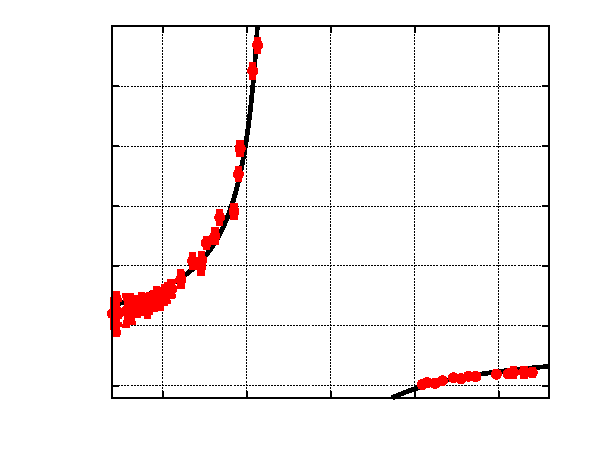
\includegraphics{HDLGuinierRadius}}%
    \gplfronttext
  \end{picture}%
\endgroup

		\caption{Squared radius of the HDL scattering data. The analytical fit results in an average density of 353.6 nm$^{-3}$ and an external diameter of 12 nm.}
		\label{fig:HDLGuinierRadius}
\end{figure}

Another model-free interpretation of the HDL scattering data is presented in figure \ref{fig:HDLGuinierRadius}, where the the squared radius of the Guinier region is presented as a function of the solvent electron density. As previously shown, the analytical expression \textcolor{red}{REF EQ} can be fitted to the experimental data, resulting in an average electron density $\rho_0=353.6$ nm$^{-3}$ and a particle shape radius of $R_c=6$ nm. The size obtained with this approach, 12 nm, is consistent with the previous result. Probably because of the absence of relevant experimental points around the match point, the average density differs in almost 5 nm$^{-3}$ from the $I(0)$ result.

The continuous contrast variation technique and the subsequent model-free analysis are easy and effective tools to measure the size and density of lipoproteins, very important attributes to understand the biological processes related to cholesterol and lipid transport. A more detailed analysis and modelling of the scattering data could have addressed some issues such as the hydration and distribution of the proteins on the surface, the permeability of the steric and lipid core or the radial distribution of cholesterol and triglycerides in the lipoprotein. However, the focus of our study was principally on the most distinctive traits of the lipoprotein classes: density and size.


\section{Protein-coated low-density nanoparticles}
\label{sec:CoatedKiskerExperimental}
The most recent efforts in nanomedicine aim for a high control of the nanocarrier surface, as the surface's properties are a defining element of its efficiency as drug carrier. Besides, nanoparticles interact with proteins when introduced into biological media, leading to the formation of the so-called \emph{protein corona} surrounding the nanocarrier \cite{cedervall_understanding_2007,monopoli_physicalchemical_2011,casals_time_2010}. The identity of the biomolecule coating depends on the particle size, surface functionalization and charge \cite{lundqvist_nanoparticle_2008,tenzer_rapid_2013,gessner_functional_2003} and its detailed description is challenging. Yet, the ability to quantitatively characterise this interface is important in understanding particle behaviour in these complex environments and improving their surface engineering for enhanced functionality.

Immunoglobulin G (IgG) is the most common type of antibody found in human serum and, therefore, a logical candidate to coat the studied nanoparticles with. In this case, we used comercially available PS-COOH particles, because polystyrene is a frequent material in nanomedicine strategies and has a wide variety of possible surface functionalizations. The carboxylated surface prevents the agglomeration of the particles and also provides a chemical anchor for the protein binding. The use of SAXS to obtain a quantitative description of the protein corona is examined for different IgG concentrations, e.g. shell thicknesses, and compared with DLS and DCS \cite{minelli_characterization_2014}.

\begin{figure}
	\centering
		% GNUPLOT: LaTeX picture with Postscript
\begingroup
  \makeatletter
  \providecommand\color[2][]{%
    \GenericError{(gnuplot) \space\space\space\@spaces}{%
      Package color not loaded in conjunction with
      terminal option `colourtext'%
    }{See the gnuplot documentation for explanation.%
    }{Either use 'blacktext' in gnuplot or load the package
      color.sty in LaTeX.}%
    \renewcommand\color[2][]{}%
  }%
  \providecommand\includegraphics[2][]{%
    \GenericError{(gnuplot) \space\space\space\@spaces}{%
      Package graphicx or graphics not loaded%
    }{See the gnuplot documentation for explanation.%
    }{The gnuplot epslatex terminal needs graphicx.sty or graphics.sty.}%
    \renewcommand\includegraphics[2][]{}%
  }%
  \providecommand\rotatebox[2]{#2}%
  \@ifundefined{ifGPcolor}{%
    \newif\ifGPcolor
    \GPcolortrue
  }{}%
  \@ifundefined{ifGPblacktext}{%
    \newif\ifGPblacktext
    \GPblacktextfalse
  }{}%
  % define a \g@addto@macro without @ in the name:
  \let\gplgaddtomacro\g@addto@macro
  % define empty templates for all commands taking text:
  \gdef\gplbacktext{}%
  \gdef\gplfronttext{}%
  \makeatother
  \ifGPblacktext
    % no textcolor at all
    \def\colorrgb#1{}%
    \def\colorgray#1{}%
  \else
    % gray or color?
    \ifGPcolor
      \def\colorrgb#1{\color[rgb]{#1}}%
      \def\colorgray#1{\color[gray]{#1}}%
      \expandafter\def\csname LTw\endcsname{\color{white}}%
      \expandafter\def\csname LTb\endcsname{\color{black}}%
      \expandafter\def\csname LTa\endcsname{\color{black}}%
      \expandafter\def\csname LT0\endcsname{\color[rgb]{1,0,0}}%
      \expandafter\def\csname LT1\endcsname{\color[rgb]{0,1,0}}%
      \expandafter\def\csname LT2\endcsname{\color[rgb]{0,0,1}}%
      \expandafter\def\csname LT3\endcsname{\color[rgb]{1,0,1}}%
      \expandafter\def\csname LT4\endcsname{\color[rgb]{0,1,1}}%
      \expandafter\def\csname LT5\endcsname{\color[rgb]{1,1,0}}%
      \expandafter\def\csname LT6\endcsname{\color[rgb]{0,0,0}}%
      \expandafter\def\csname LT7\endcsname{\color[rgb]{1,0.3,0}}%
      \expandafter\def\csname LT8\endcsname{\color[rgb]{0.5,0.5,0.5}}%
    \else
      % gray
      \def\colorrgb#1{\color{black}}%
      \def\colorgray#1{\color[gray]{#1}}%
      \expandafter\def\csname LTw\endcsname{\color{white}}%
      \expandafter\def\csname LTb\endcsname{\color{black}}%
      \expandafter\def\csname LTa\endcsname{\color{black}}%
      \expandafter\def\csname LT0\endcsname{\color{black}}%
      \expandafter\def\csname LT1\endcsname{\color{black}}%
      \expandafter\def\csname LT2\endcsname{\color{black}}%
      \expandafter\def\csname LT3\endcsname{\color{black}}%
      \expandafter\def\csname LT4\endcsname{\color{black}}%
      \expandafter\def\csname LT5\endcsname{\color{black}}%
      \expandafter\def\csname LT6\endcsname{\color{black}}%
      \expandafter\def\csname LT7\endcsname{\color{black}}%
      \expandafter\def\csname LT8\endcsname{\color{black}}%
    \fi
  \fi
    \setlength{\unitlength}{0.0500bp}%
    \ifx\gptboxheight\undefined%
      \newlength{\gptboxheight}%
      \newlength{\gptboxwidth}%
      \newsavebox{\gptboxtext}%
    \fi%
    \setlength{\fboxrule}{0.5pt}%
    \setlength{\fboxsep}{1pt}%
\begin{picture}(5668.00,4534.00)%
    \gplgaddtomacro\gplbacktext{%
      \csname LTb\endcsname%
      \put(726,638){\makebox(0,0)[r]{\strut{}$1$}}%
      \csname LTb\endcsname%
      \put(726,1848){\makebox(0,0)[r]{\strut{}$10$}}%
      \csname LTb\endcsname%
      \put(726,3059){\makebox(0,0)[r]{\strut{}$100$}}%
      \csname LTb\endcsname%
      \put(726,4269){\makebox(0,0)[r]{\strut{}$1000$}}%
      \csname LTb\endcsname%
      \put(944,418){\makebox(0,0){\strut{}$0.03$}}%
      \csname LTb\endcsname%
      \put(1797,418){\makebox(0,0){\strut{}$0.05$}}%
      \csname LTb\endcsname%
      \put(2955,418){\makebox(0,0){\strut{}$0.1$}}%
      \csname LTb\endcsname%
      \put(4113,418){\makebox(0,0){\strut{}$0.2$}}%
      \csname LTb\endcsname%
      \put(5271,418){\makebox(0,0){\strut{}$0.4$}}%
    }%
    \gplgaddtomacro\gplfronttext{%
      \csname LTb\endcsname%
      \put(220,2453){\rotatebox{-270}{\makebox(0,0){\strut{}Scattering Intensity / a.u.}}}%
      \put(3064,154){\makebox(0,0){\strut{}$q$ / nm$^{-1}$}}%
      \csname LTb\endcsname%
      \put(4548,4041){\makebox(0,0)[r]{\strut{}\smaller PS-COOH}}%
      \csname LTb\endcsname%
      \put(4548,3711){\makebox(0,0)[r]{\strut{}\smaller 0.5 mg/ml IgG}}%
      \csname LTb\endcsname%
      \put(4548,3381){\makebox(0,0)[r]{\strut{}\smaller 1 mg/ml IgG}}%
      \csname LTb\endcsname%
      \put(4548,3051){\makebox(0,0)[r]{\strut{}\smaller 2 mg/ml IgG}}%
      \csname LTb\endcsname%
      \put(4548,2721){\makebox(0,0)[r]{\strut{}\smaller 4 mg/ml IgG}}%
    }%
    \gplbacktext
    \put(0,0){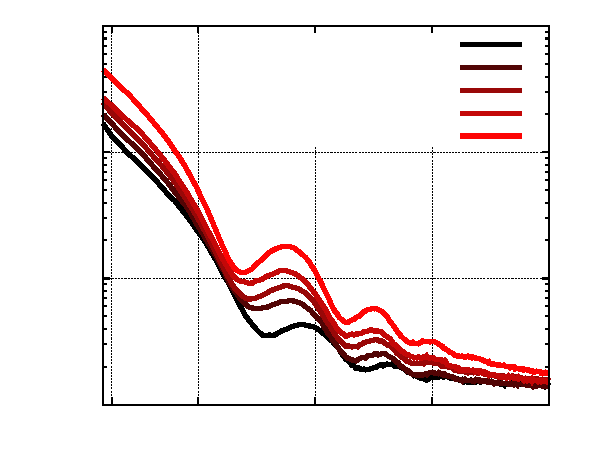
\includegraphics{CoatedKiskerIgGSingleContrastSAXS}}%
    \gplfronttext
  \end{picture}%
\endgroup

		\caption{SAXS curves at a single contrast of PS-COOH particles coated with IgG at different concentrations.}
		\label{fig:CoatedKiskerIgGSingleContrastSAXS}
\end{figure}

The bare PS-COOH particles are highly charged, showing a $\zeta$-potential of ($-49 \pm 1$) mV, which is drastically reduced to around $ -10$ mV following the binding of the positively charged IgG. The SAXS measurements of the IgG-coated particles with different protein concentrations are shown in figure \ref{fig:CoatedKiskerIgGSingleContrastSAXS}, where a clear shift to smaller $q$-values is observed for increasing concentration of IgG. This effect is clearly related with the increase in size for higher IgG concentration, although a quantitative description is complicated.

Due to the core-shell morphology of the polymeric bare particle (see \textcolor{red}{PREVIOUS SECTION}), SAXS curves were analyzed using a double-shell model (see \textcolor{red}{EXPRESSION IN SECTION}), considering a sharp interface between the different components and a constant thickness and density of the IgG corona. In order to focus on the total diameter instead of the details of the internal structure, the limits of the inner and outer radii of the polymer shell are not fixed and are treated as fitting parameters together with the outer radius and the contrast difference of each shell with the polystyrene core.

\begin{table}[]
\centering
\caption{Concentration of IgG incubated with PS-COOH particles and IgG shell thickness as measured by single-contrast SAXS, DCS and DLS \cite{minelli_characterization_2014}. A double-shell model with sharp interfaces was used for the SAXS results. The uncertainties are the standard deviations of repeated measurements.}
\label{tab:CoatedKiskerSingleContrast}
\begin{tabular}{|c|c|c|c|c|}
\hline
\multicolumn{1}{|l|}{\textbf{$\rho_{IgG}$ / mg mL$^{-1}$ }} & \multicolumn{1}{l|}{\textbf{$\zeta$-potential / mV}} & \multicolumn{1}{l|}{\textbf{T$_{DLS}$ / nm}} & \multicolumn{1}{l|}{\textbf{T$_{DCS}$ / nm}} & \multicolumn{1}{l|}{\textbf{T$_{SAXS}$ / nm}} \\ \hline
0.5                     & -10.8 $\pm$ 0.9                  & 10 $\pm$ 1              & 3.7 $\pm$ 0.6                                & 7.7 $\pm$ 1.4                                 \\ \hline
1                        & -10.7 $\pm$ 0.6                  & 11 $\pm$ 2              & 5.9 $\pm$ 0.5                                & 8.4 $\pm$ 1.4                                 \\ \hline
2                         & -9.6 $\pm$ 0.5                   & 12 $\pm$ 2              & 7.6 $\pm$ 0.4                                & 9.6 $\pm$ 1.5                                 \\ \hline
4                        & -9.7 $\pm$ 0.5                   & 15 $\pm$ 2              & 8.3 $\pm$ 0.4                                & 9.6 $\pm$ 1.5                                 \\ \hline
\end{tabular}
\end{table}

The IgG shell thickness obtained for IgG-coated particles with different protein concentrations is shown in table \ref{tab:CoatedKiskerSingleContrast} and compared to the size measurements performed with other techniques. All DLS, DCS and SAXS techniques show an increase in the IgG-shell thickness with increasing concentration of the protein in solution during incubation. As expected, DLS provides higher values than the other techniques, as the measured thickness is related to the hydrodynamic properties of the system.

Although all techniques show an increase of the IgG shell thickness with increasing concentration of the protein, full consistency among them requires further refinements of the SAXS and DCS modelling. For instance, the SAXS evaluation has neglected the possible spatial heterogeneity and hydration of the IgG corona and the model employed for the core particle overstimates the size in almost 10 $\%$ \cite{minelli_characterization_2014, garcia-diez_nanoparticle_2015}.

\subsection{Hard protein corona characterization with contrast variation}
\label{sec:coated_kisker_continuous}

\begin{figure}
	\centering
		% GNUPLOT: LaTeX picture with Postscript
\begingroup
  \makeatletter
  \providecommand\color[2][]{%
    \GenericError{(gnuplot) \space\space\space\@spaces}{%
      Package color not loaded in conjunction with
      terminal option `colourtext'%
    }{See the gnuplot documentation for explanation.%
    }{Either use 'blacktext' in gnuplot or load the package
      color.sty in LaTeX.}%
    \renewcommand\color[2][]{}%
  }%
  \providecommand\includegraphics[2][]{%
    \GenericError{(gnuplot) \space\space\space\@spaces}{%
      Package graphicx or graphics not loaded%
    }{See the gnuplot documentation for explanation.%
    }{The gnuplot epslatex terminal needs graphicx.sty or graphics.sty.}%
    \renewcommand\includegraphics[2][]{}%
  }%
  \providecommand\rotatebox[2]{#2}%
  \@ifundefined{ifGPcolor}{%
    \newif\ifGPcolor
    \GPcolortrue
  }{}%
  \@ifundefined{ifGPblacktext}{%
    \newif\ifGPblacktext
    \GPblacktextfalse
  }{}%
  % define a \g@addto@macro without @ in the name:
  \let\gplgaddtomacro\g@addto@macro
  % define empty templates for all commands taking text:
  \gdef\gplbacktext{}%
  \gdef\gplfronttext{}%
  \makeatother
  \ifGPblacktext
    % no textcolor at all
    \def\colorrgb#1{}%
    \def\colorgray#1{}%
  \else
    % gray or color?
    \ifGPcolor
      \def\colorrgb#1{\color[rgb]{#1}}%
      \def\colorgray#1{\color[gray]{#1}}%
      \expandafter\def\csname LTw\endcsname{\color{white}}%
      \expandafter\def\csname LTb\endcsname{\color{black}}%
      \expandafter\def\csname LTa\endcsname{\color{black}}%
      \expandafter\def\csname LT0\endcsname{\color[rgb]{1,0,0}}%
      \expandafter\def\csname LT1\endcsname{\color[rgb]{0,1,0}}%
      \expandafter\def\csname LT2\endcsname{\color[rgb]{0,0,1}}%
      \expandafter\def\csname LT3\endcsname{\color[rgb]{1,0,1}}%
      \expandafter\def\csname LT4\endcsname{\color[rgb]{0,1,1}}%
      \expandafter\def\csname LT5\endcsname{\color[rgb]{1,1,0}}%
      \expandafter\def\csname LT6\endcsname{\color[rgb]{0,0,0}}%
      \expandafter\def\csname LT7\endcsname{\color[rgb]{1,0.3,0}}%
      \expandafter\def\csname LT8\endcsname{\color[rgb]{0.5,0.5,0.5}}%
    \else
      % gray
      \def\colorrgb#1{\color{black}}%
      \def\colorgray#1{\color[gray]{#1}}%
      \expandafter\def\csname LTw\endcsname{\color{white}}%
      \expandafter\def\csname LTb\endcsname{\color{black}}%
      \expandafter\def\csname LTa\endcsname{\color{black}}%
      \expandafter\def\csname LT0\endcsname{\color{black}}%
      \expandafter\def\csname LT1\endcsname{\color{black}}%
      \expandafter\def\csname LT2\endcsname{\color{black}}%
      \expandafter\def\csname LT3\endcsname{\color{black}}%
      \expandafter\def\csname LT4\endcsname{\color{black}}%
      \expandafter\def\csname LT5\endcsname{\color{black}}%
      \expandafter\def\csname LT6\endcsname{\color{black}}%
      \expandafter\def\csname LT7\endcsname{\color{black}}%
      \expandafter\def\csname LT8\endcsname{\color{black}}%
    \fi
  \fi
    \setlength{\unitlength}{0.0500bp}%
    \ifx\gptboxheight\undefined%
      \newlength{\gptboxheight}%
      \newlength{\gptboxwidth}%
      \newsavebox{\gptboxtext}%
    \fi%
    \setlength{\fboxrule}{0.5pt}%
    \setlength{\fboxsep}{1pt}%
\begin{picture}(5668.00,4534.00)%
    \gplgaddtomacro\gplbacktext{%
      \csname LTb\endcsname%
      \put(594,1690){\makebox(0,0)[r]{\strut{}$0.1$}}%
      \csname LTb\endcsname%
      \put(594,4166){\makebox(0,0)[r]{\strut{}$1$}}%
      \csname LTb\endcsname%
      \put(1346,484){\makebox(0,0){\strut{}$0.075$}}%
      \csname LTb\endcsname%
      \put(2379,484){\makebox(0,0){\strut{}$0.1$}}%
      \csname LTb\endcsname%
      \put(3412,484){\makebox(0,0){\strut{}$0.125$}}%
      \csname LTb\endcsname%
      \put(4445,484){\makebox(0,0){\strut{}$0.15$}}%
    }%
    \gplgaddtomacro\gplfronttext{%
      \csname LTb\endcsname%
      \put(220,2486){\rotatebox{-270}{\makebox(0,0){\strut{}Relative Standard Deviation}}}%
      \put(2998,154){\makebox(0,0){\strut{}$q$ / nm$^{-1}$}}%
      \csname LTb\endcsname%
      \put(4548,4041){\makebox(0,0)[r]{\strut{}\smaller Plain PS-COOH}}%
      \csname LTb\endcsname%
      \put(4548,3711){\makebox(0,0)[r]{\strut{}\smaller After attaching IgG}}%
    }%
    \gplbacktext
    \put(0,0){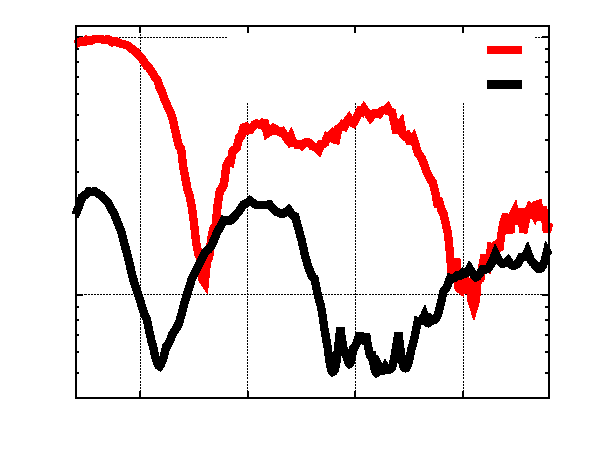
\includegraphics{CoatedKiskerIsopointComp}}%
    \gplfronttext
  \end{picture}%
\endgroup

		\caption{Isoscattering point position before and after attaching IgG (4 mg mL$^{-1}$) to the PS-COOH particles. A shift of the first minimum to lower $q$-values is observed after attaching the biotarget to the nanoparticle.}
		\label{fig:CoatedKiskerIsopointComp}
\end{figure}

The possible inaccuracies arising from the previous modelling approach might be prevented by using continuous contrast variation and a model-free evaluation. For this purpose, the protein-coated particle with 4 mg mL$^{-1}$ IgG was introduced in a density gradient with sucrose as contrast agent, resulting in an increase of the solvent electron density until 350.8 nm$^{-3}$ at the maximum sucrose concentration of 14.7 $\%$. As \textcolor{red}{DISCUSSED BEFORE}, the isoscattering point position is quantified by calculating the relative standard deviation of the 20 measured curves at each $q$, as depicted in figure \ref{fig:CoatedKiskerIsopointComp}. This value becomes minimal at $q=0.0795\pm0.0019$ nm$^{-1}$.

By comparing the relative standard deviation curves of the bare PS-COOH particle \cite{garcia-diez_nanoparticle_2015} and the IgG-coated sample (figure \ref{fig:CoatedKiskerIsopointComp}), it is noticeable that the position of the minimum is shifted to smaller $q$-values after attaching the bioprobe to the surface as a consequence of the increase in size. The diameter increase $t$ can be quantified by inserting the isoscattering positions before and after the target attachment, $q^{\star}=0.0900$ nm$^{-1}$ and $q^{\star}_{IgG}=0.0795$ nm$^{-1}$ respectively, in the equation already discussed in section  \textcolor{red}{EQUATION OF ISOSCATTERING POINT, TANQR=QR}:


\begin{equation}
t = R_{IgG} - R = \frac{K_1}{q^{\star}_{IgG}}-\frac{K_1}{q^{\star}} ,
\label{eq:IsopointRadiusDifference}
\end{equation}

where $K_1$ is a factor which depends slightly on the particle poydispersity and sphericity (typically $K_1 = 4.493$), $t$ is the IgG-shell thickness and $R$ and $R_{IgG}$ are the particle radii before and after IgG incubation. This results in a shell thickness of (6.6 $\pm$ 1.9) nm. 

It is important to highlight that this result corresponds to the volume inaccessible for the solvent (section \textcolor{red}{theory contrast variation}) and, thus, it can be identified with the hard protein corona surrounding the polymeric nanoparticle. This assumption agrees with the larger values found with other methods in table \ref{tab:CoatedKiskerSingleContrast}, which probe the permeable part of the IgG shell as well. The hard corona has a thickness of (6.6 $\pm$ 1.9) nm, around 2 nm thinner than the complete protein layer.

\subsubsection{Uncertainty analysis}
The associated uncertainty to the isoscattering point position $q^{\star}$ of 0.0019 nm$^{-1}$ depends on the chosen $q$-bin size, the correction of the background contributions from the solvent \cite{garcia-diez_nanoparticle_2015}, the energy resolution of the photon beam \cite{krumrey_high-accuracy_2001}, the accuracy of the distance between the irradiated sample and the scattering detector, the detector pixel size \cite{wernecke_characterization_2014} or the determination of the scattering center. Each contribution to the uncertainty budget has been detailled in table \ref{tab:IsopointUncertainty}, where the contribution of the selected $q$-bin size is the largest. The uncertainties given are standard uncertainties ($k = 1$)

\begin{table}[]
\centering
\caption{Uncertainty contributions associated to the isoscattering point $q^{\star}$ position, where $u_I$ and $u_r$ correspond to the input uncertainty and relative uncertainty respectively.}
\label{tab:IsopointUncertainty}
\begin{tabular}{|l|c|c|c|}
\hline
\multicolumn{1}{|c|}{\textbf{Input quantity}} & \textbf{$u_I$} & \textbf{$u_r$} & \multicolumn{1}{l|}{\textbf{Contribution}} \\ \hline
Photon Energy                   & 0.8 eV                     & 10$^{-4}$                          & 0.000008 nm$^{-1}$                                                      \\ \hline
Sample-detector distance           & 5 mm                       & 10$^{-3}$                          & 0.00008 nm$^{-1}$                                                       \\ \hline
Pixel size                      & 0.2 $\mu$m                     & 10$^{-3}$                          & 0.00008 nm$^{-1}$                                                       \\ \hline
Center determination               & n.a.                       & n.a.                          & 0.0008 nm$^{-1}$                                                        \\ \hline
$q$-bin size                      & 0.0015 nm$^{-1}$              & $2\cdot 10^{-2}$                        & 0.0015 nm$^{-1}$                                                        \\ \hline
Solvent background              & n.a.                       & n.a.                          & 0.0009 nm$^{-1}$                                                        \\ \hline
\multicolumn{3}{|l|}{\textbf{\begin{tabular}[c]{@{}l@{}}Combined standard uncertainty\end{tabular}}}                             & \textbf{0.0019 nm$^{-1}$}                                                        \\ \hline
\end{tabular}
\end{table}

The uncertainty associated to the thickness of the protein layer $t$ produces a limit of detection of 1.9 nm, which arises from the previously discussed $q^{\star}$ uncertainty and an uncertainty of 10 $\%$ associated with the particle polydispersity and reflected in $K_1$. From the expression \ref{eq:IsopointRadiusDifference}, the thickness uncertainty $\delta t$ can be derived as:

\begin{equation}
\delta t^2 = \left( t \frac{\delta K_1}{K_1} \right)^2 + \left( \frac{K_1}{\left(q^{\star}_{IgG}\right)^2} \delta q^{\star}_{IgG} \right)^2 + \left( \frac{K_1}{\left(q^{\star}\right)^2} \delta q^{\star}\right)^2
\end{equation}

where $\delta q^{\star}_{IgG}=\delta q^{\star}=0.0019$ nm$^{-1}$.

\section{Summary}
The results presented in this section demonstrate that it is possible to determine the size of complicated nanoparticles relevant in nanomedicine with continuous contrast variation in SAXS. This technique has been used to characterize a great variety of systems in the nanoscale such as the PEGylated liposomal nanodrug Caelyx$\textregistered$, empty liposomal nanocarriers, human lipoproteins or protein-coated polymeric nanoparticles.

In the case of Caelyx$\textregistered$, by means of an iso-osmolal density gradient, the position of the isoscattering point was measured whereby the size of the liposomal drug was determined with this model-free approach. Supplemented by the model fitting of the so called \emph{shape factor} of the liposomes, the size was also obtained from an independent evaluation procedure and an average size of (69 $\pm$ 5) nm was obtained. This size is smaller than the value measured by DLS, which can be attributed to the fact that the contrast variation SAXS determines the size of the liposomes impermeable to the contrast agent, i.e. the outer PEG layer of the liposomes is not probed. The latter implies that the combination of SAXS with DLS can reveal the difference between the hydrodynamic diameter and the "core" size of the nanocarrier, which is related to the thickness of the PEG-layer in case of stealth liposomes. Moreover it is shown that by means of the shape factor fitting, complementary information about the shape of the nanocarrier can be obtained. Complementary, it was found that the average electron density of the liposomal doxorubicin was higher than that of the empty PEGylated liposomes.

Besides, using an aqueous sucrose density gradient, it was possible to study the behavior of the liposomal drug carrier under different osmotic conditions. It was shown that an increasing osmolality of the buffer produces an osmotic shrinkage of the liposomal structure, although this structural deformation is reversible and does not affect the crystalline structure of the intraliposomal doxorubicin.

For comparison purposes with the liposomal doxorubicin system, the osmotic activity of empty liposomes was also investigated using aqueous sucrose. The distinguishable osmotic effects observed in PEGylated and plain liposomes arise from the different formation of the liposomes, which is influenced by the presence of PEG moieties in the preparation. The MLV structure of the plain liposomes show higher resiliance against osmotic pressure that the unilamellar membrane of the PEGylated vesicles. In the latter, the ULV structure shrinks due to the osmotic pressure and deforms the liposomes into obloid ellipsoids, creating a bilamellar structure at the outest part of the vesicles.

The continuous contrast variation technique was used to determine the most distinctive traits of human lipoproteins: size and density, the latter being fundamental to classify them. The parameters obtained by means of a model-free analysis are in good agreement with the reported values in literature.

Finally, the application of the technique on nanoparticles incubated in different concentrations of IgG reveals the difference between the IgG-shell and the hard protein-corona impenetrable for the solvent, probed with contrast variation SAXS. In addition, the use of complementary techniques such as DLS, SAXS and DCS show an increase of the protein-shell thickness with increasing concentration of the proteins during incubation. The SAXS contribution to this study requires of a model refinement for full consistency with the results measured for the bare PS-COOH particle.
